\section{Montagem Laboratorial}

\subsection{Implementação no Quartus e na Placa DE10-Lite}

A implementação do circuito para o cálculo do quadrado de números naturais foi realizada utilizando a linguagem \Gls{vhdl} no software  desenvolvido pela Intel. O projeto foi estruturado em etapas, começando pelo desenvolvimento do código, seguido pela simulação para validação lógica e, finalmente, a síntese do circuito para implementação na placa DE10-Lite.

\begin{figure}[H]
    \centering
    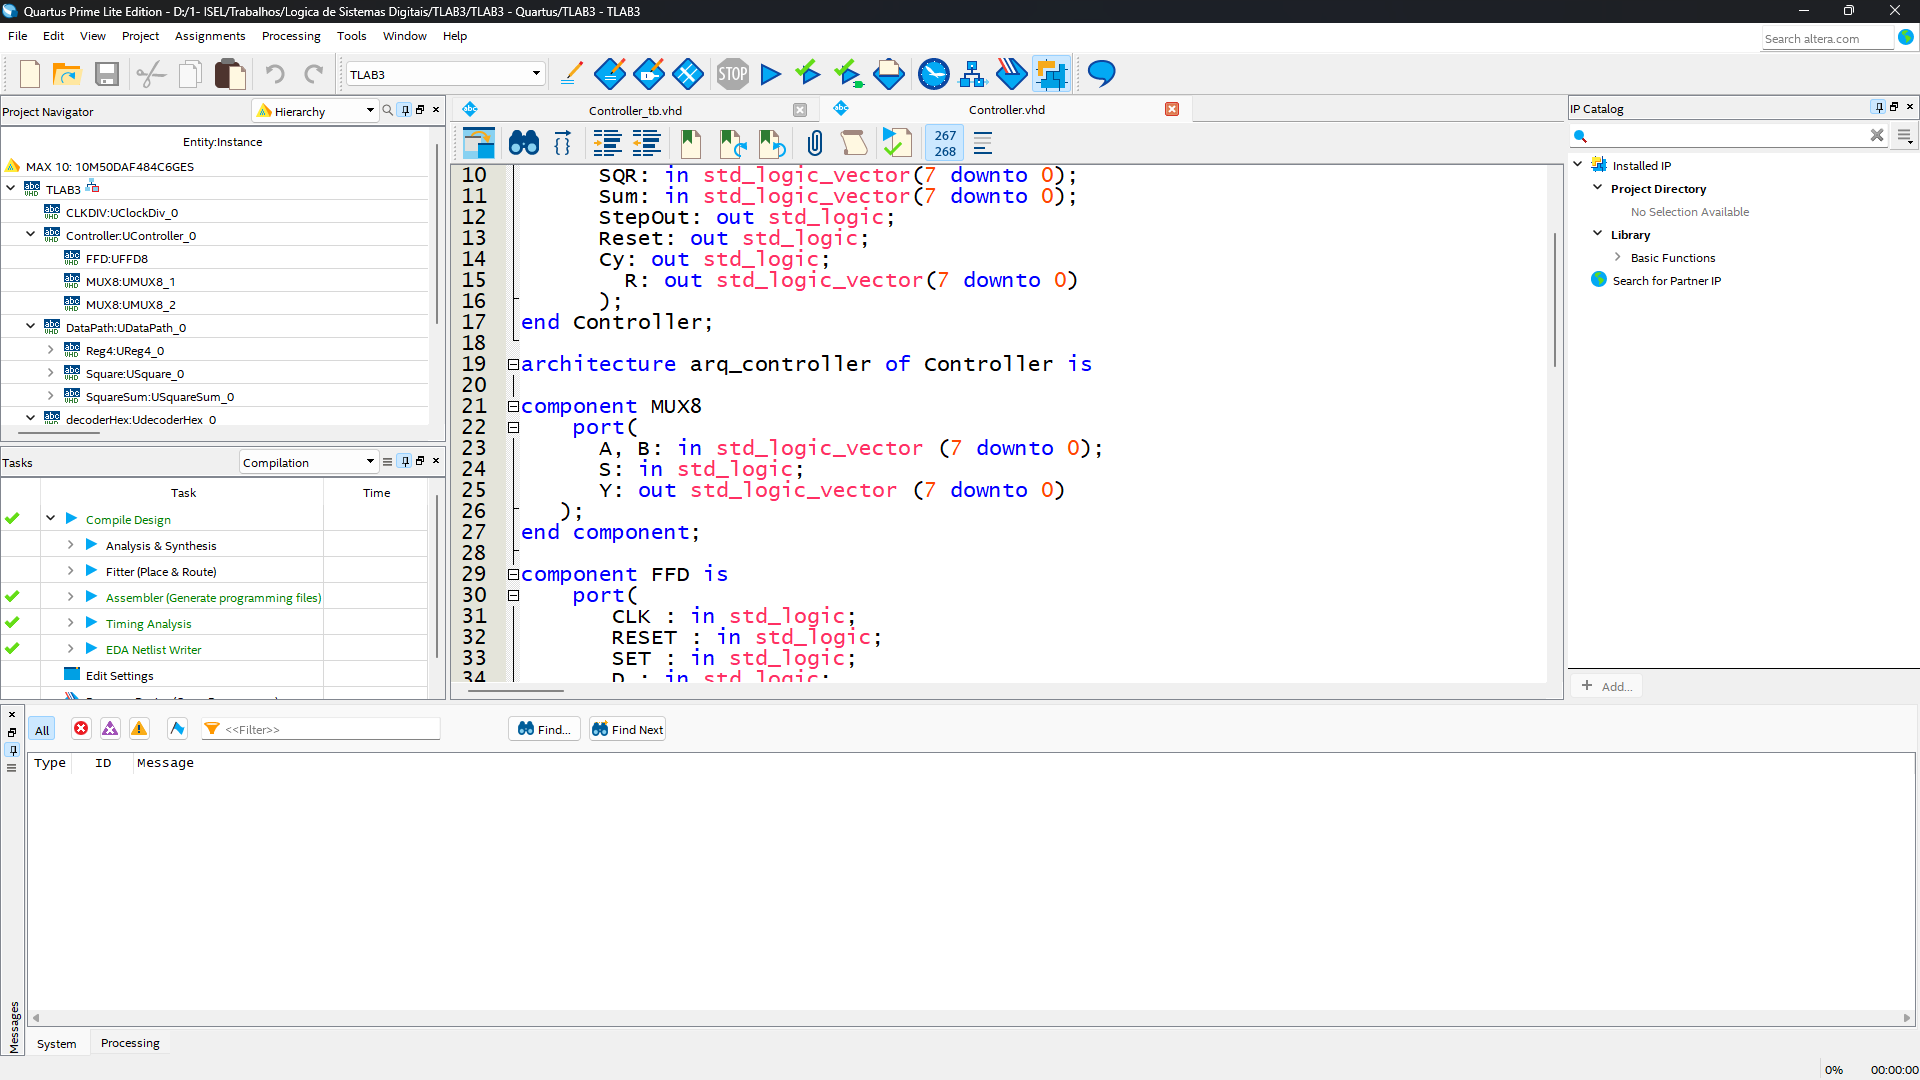
\includegraphics[width=.8\linewidth]{Montagem Laboratorial/images/Quartus.png}
    \caption{Aplicação \textit{Quartus} com o projeto aberto}\label{fig:label1}
\end{figure}

\subsubsection{Implementação}

Devido à complexidade deste trabalho relativamente ao módulos que tivemos de desenvolver, usámos como auxílio, o site CircuitVerse, onde montámos todo o nosso circuito, esquematizado por partes e funcional. Tudo isto, serviu para uma melhor compreensão do circuito a construir e ajudar no raciocínio que tivemos de adotar no desenvolver do projeto. Principalmente, facilitou a passagem dos elementos e características do circuito que montámos, previamente, no CircuitVerse, para a linguagem \Gls{vhdl}, implementada no programa \textit{Quartus} da Intel.

O código \Gls{vhdl} foi elaborado de forma modular, permitindo uma abordagem organizada e eficiente. Após a conclusão do código, utilizou-se o simulador integrado do \textit{Quartus} para verificar a funcionalidade do circuito com diversas combinações de entrada.

Com o circuito validado na simulação, procedeu-se à síntese da configuração da placa DE10-Lite. Essa etapa envolveu a aplicação das entradas e saídas físicas da placa, como \textit{switches} para os valores de entrada, \textit{displays} de 7 segmentos e um \gls{led}, para exibir os resultados. O mapeamento foi configurado no \textit{Pin Planner} do \textit{Quartus}, assegurando uma correspondência correta entre as entradas e saídas lógicas do circuito e os pinos físicos da placa.

Por fim, o design foi programado na DE10-Lite. Após o carregamento bem-sucedido do circuito na placa, alguns testes foram realizados, confirmando a operação correta do circuito e o cumprimento dos objetivos propostos inicialmente pelo enunciado.

\begin{figure}[H]
    \centering
    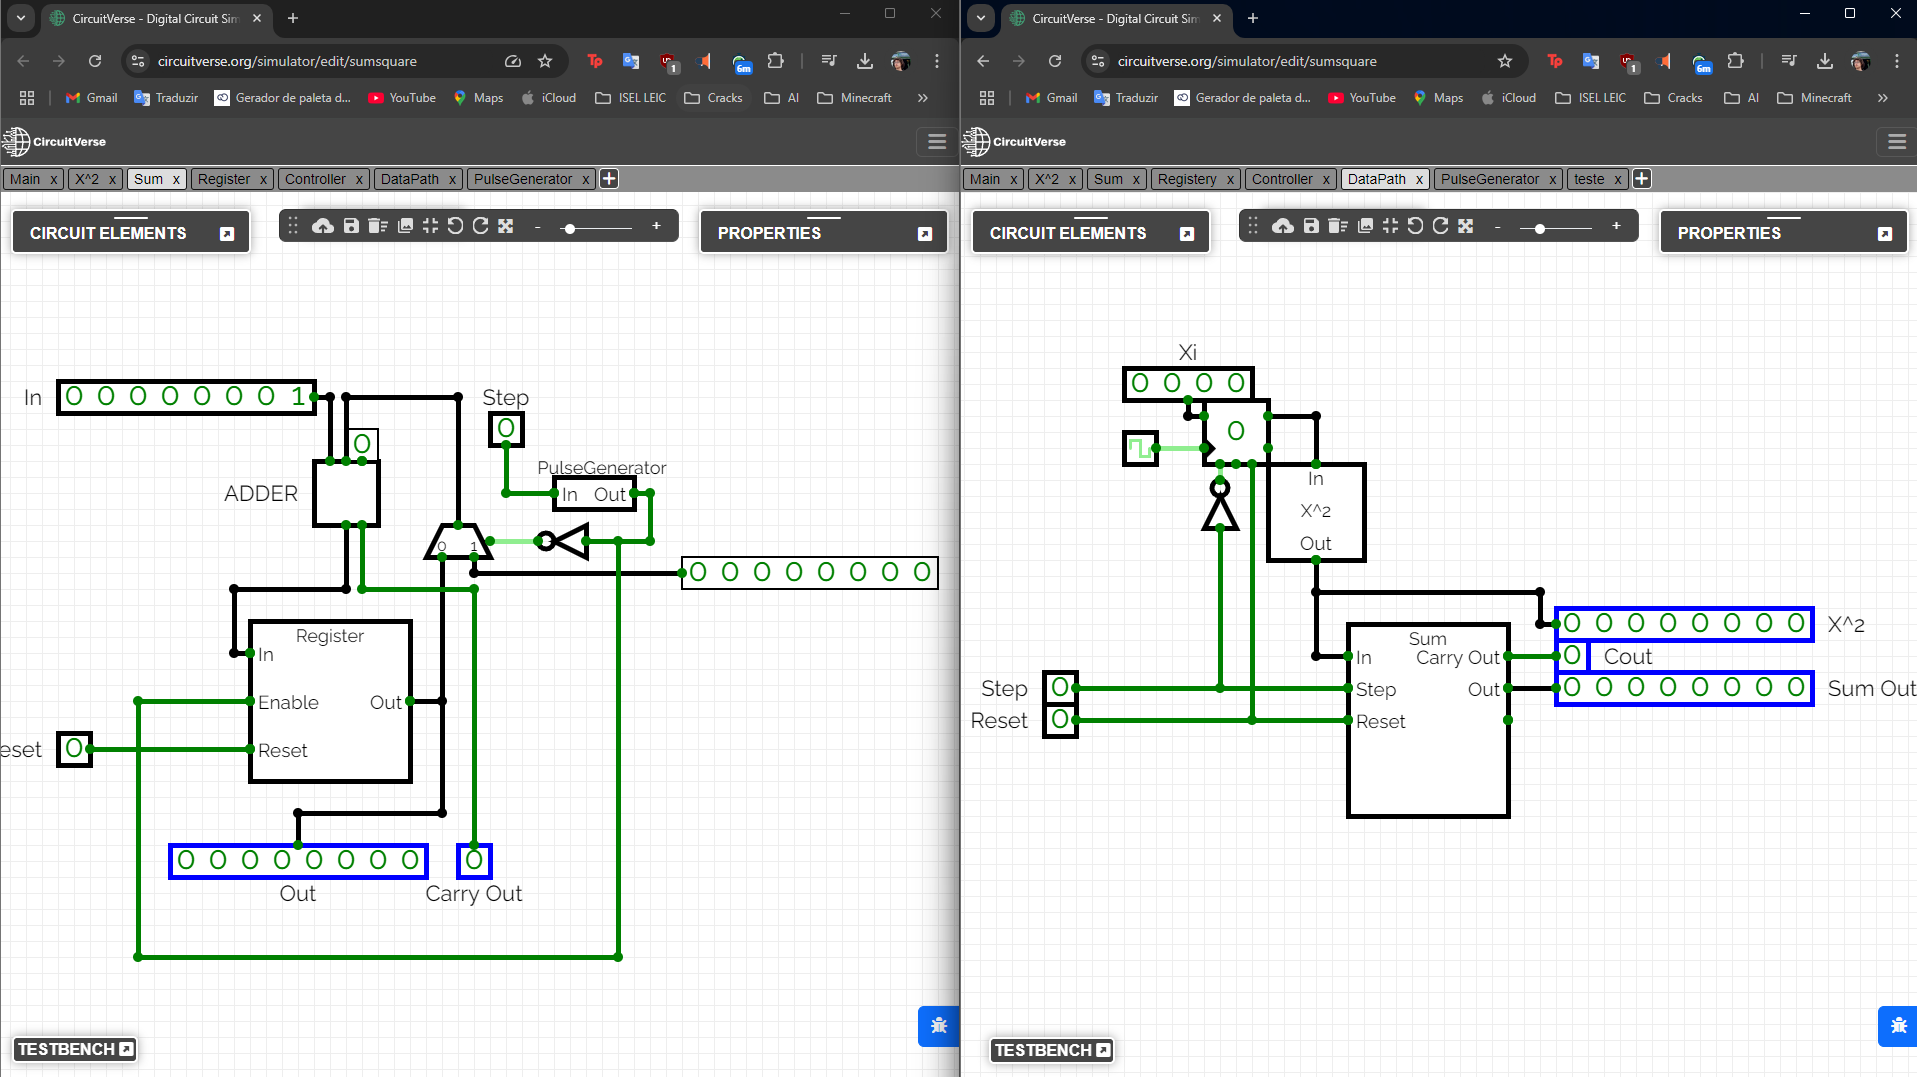
\includegraphics[width=.8\linewidth]{Montagem Laboratorial/images/CircuitVerse.png}
    \caption{Desenvolvimento da lógica no \textit{Circuit Verse}}\label{fig:enter-label}
\end{figure}

\subsubsection{Testes e Simulação}

Para a simulação deste trabalho, optou-se pelo teste a partir de casos particulares. Como inicialmente implementamos o projeto no \textit{CircuitVerse}, também fizemos os primeiros testes lá. Nas figuras~\ref{fig:CV1} a~\ref{fig:CV6} abaixo, é possível visualizar os resultados experimentais obtidos. Nos casos seguintes, o valor representado nos \textit{displays} de 7 segmentos é o valor em hexadecimal.

\begin{multicols}{2}
    \begin{figure}[H]
        \centering
        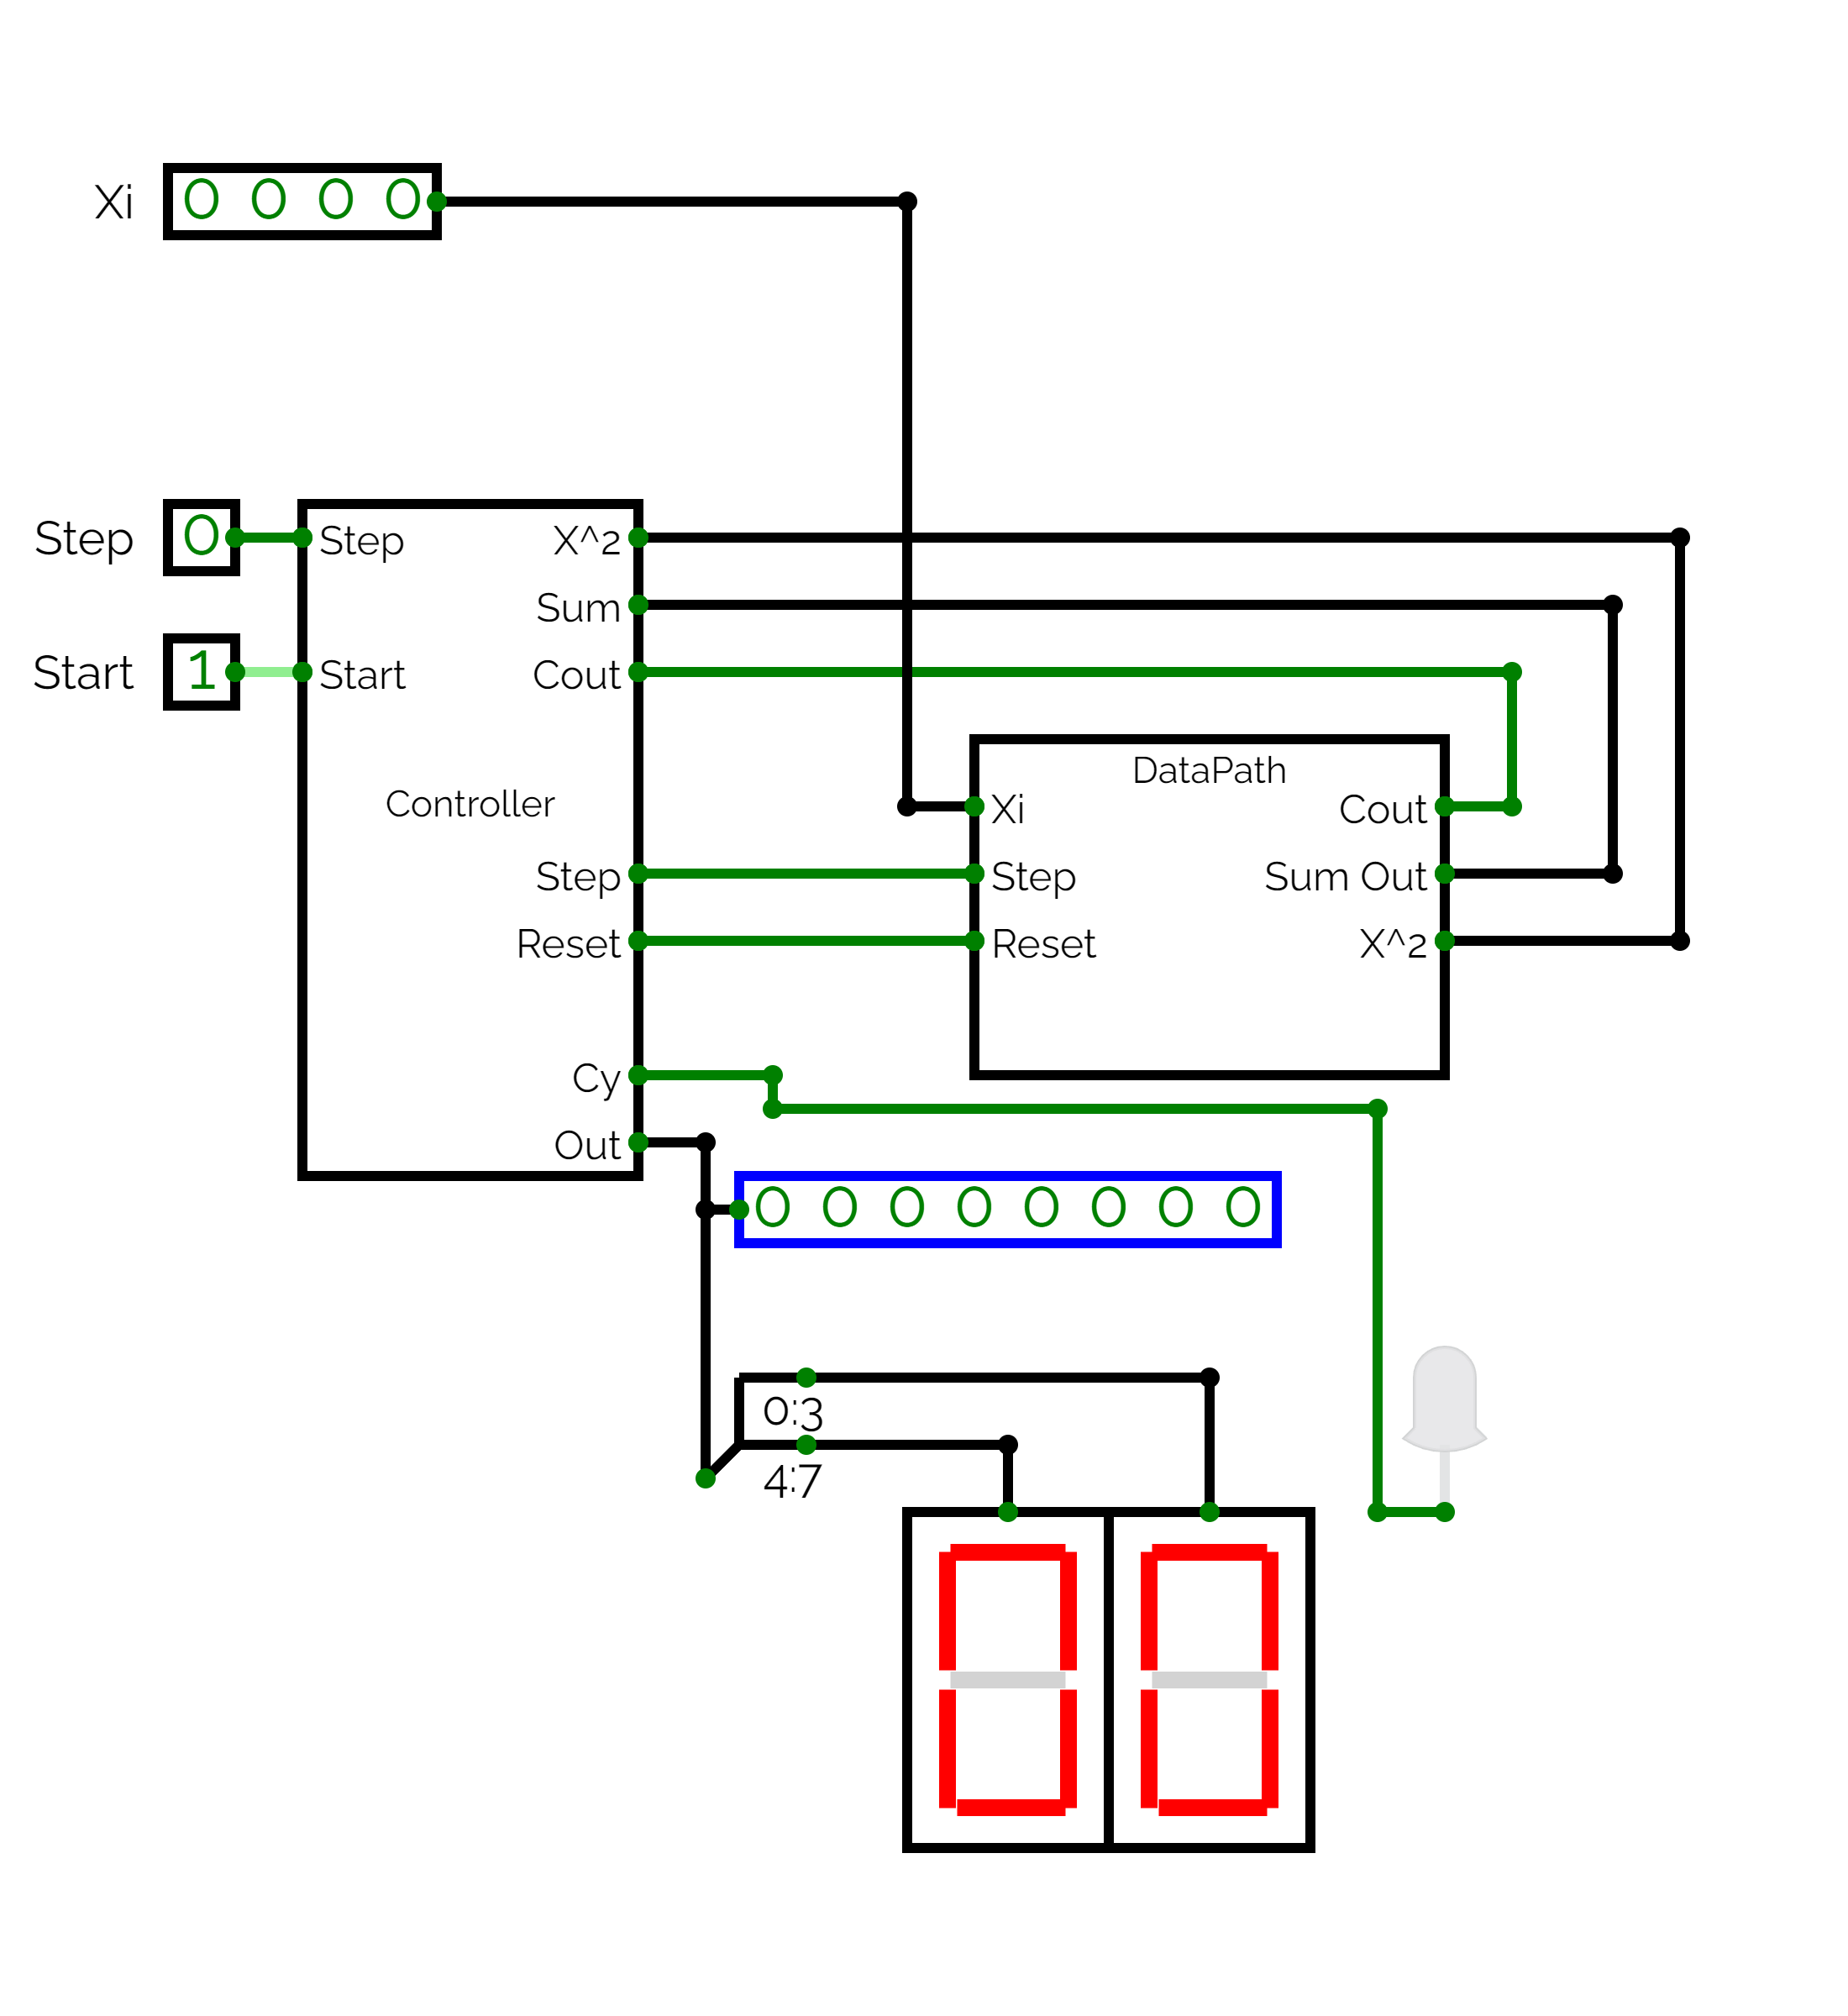
\includegraphics[scale=.08]{Montagem Laboratorial/images/Main (1).png}
        \caption{Teste no \textit{CircuitVerse} (1)}\label{fig:CV1}
    \end{figure}
    \begin{figure}[H]
        \centering
        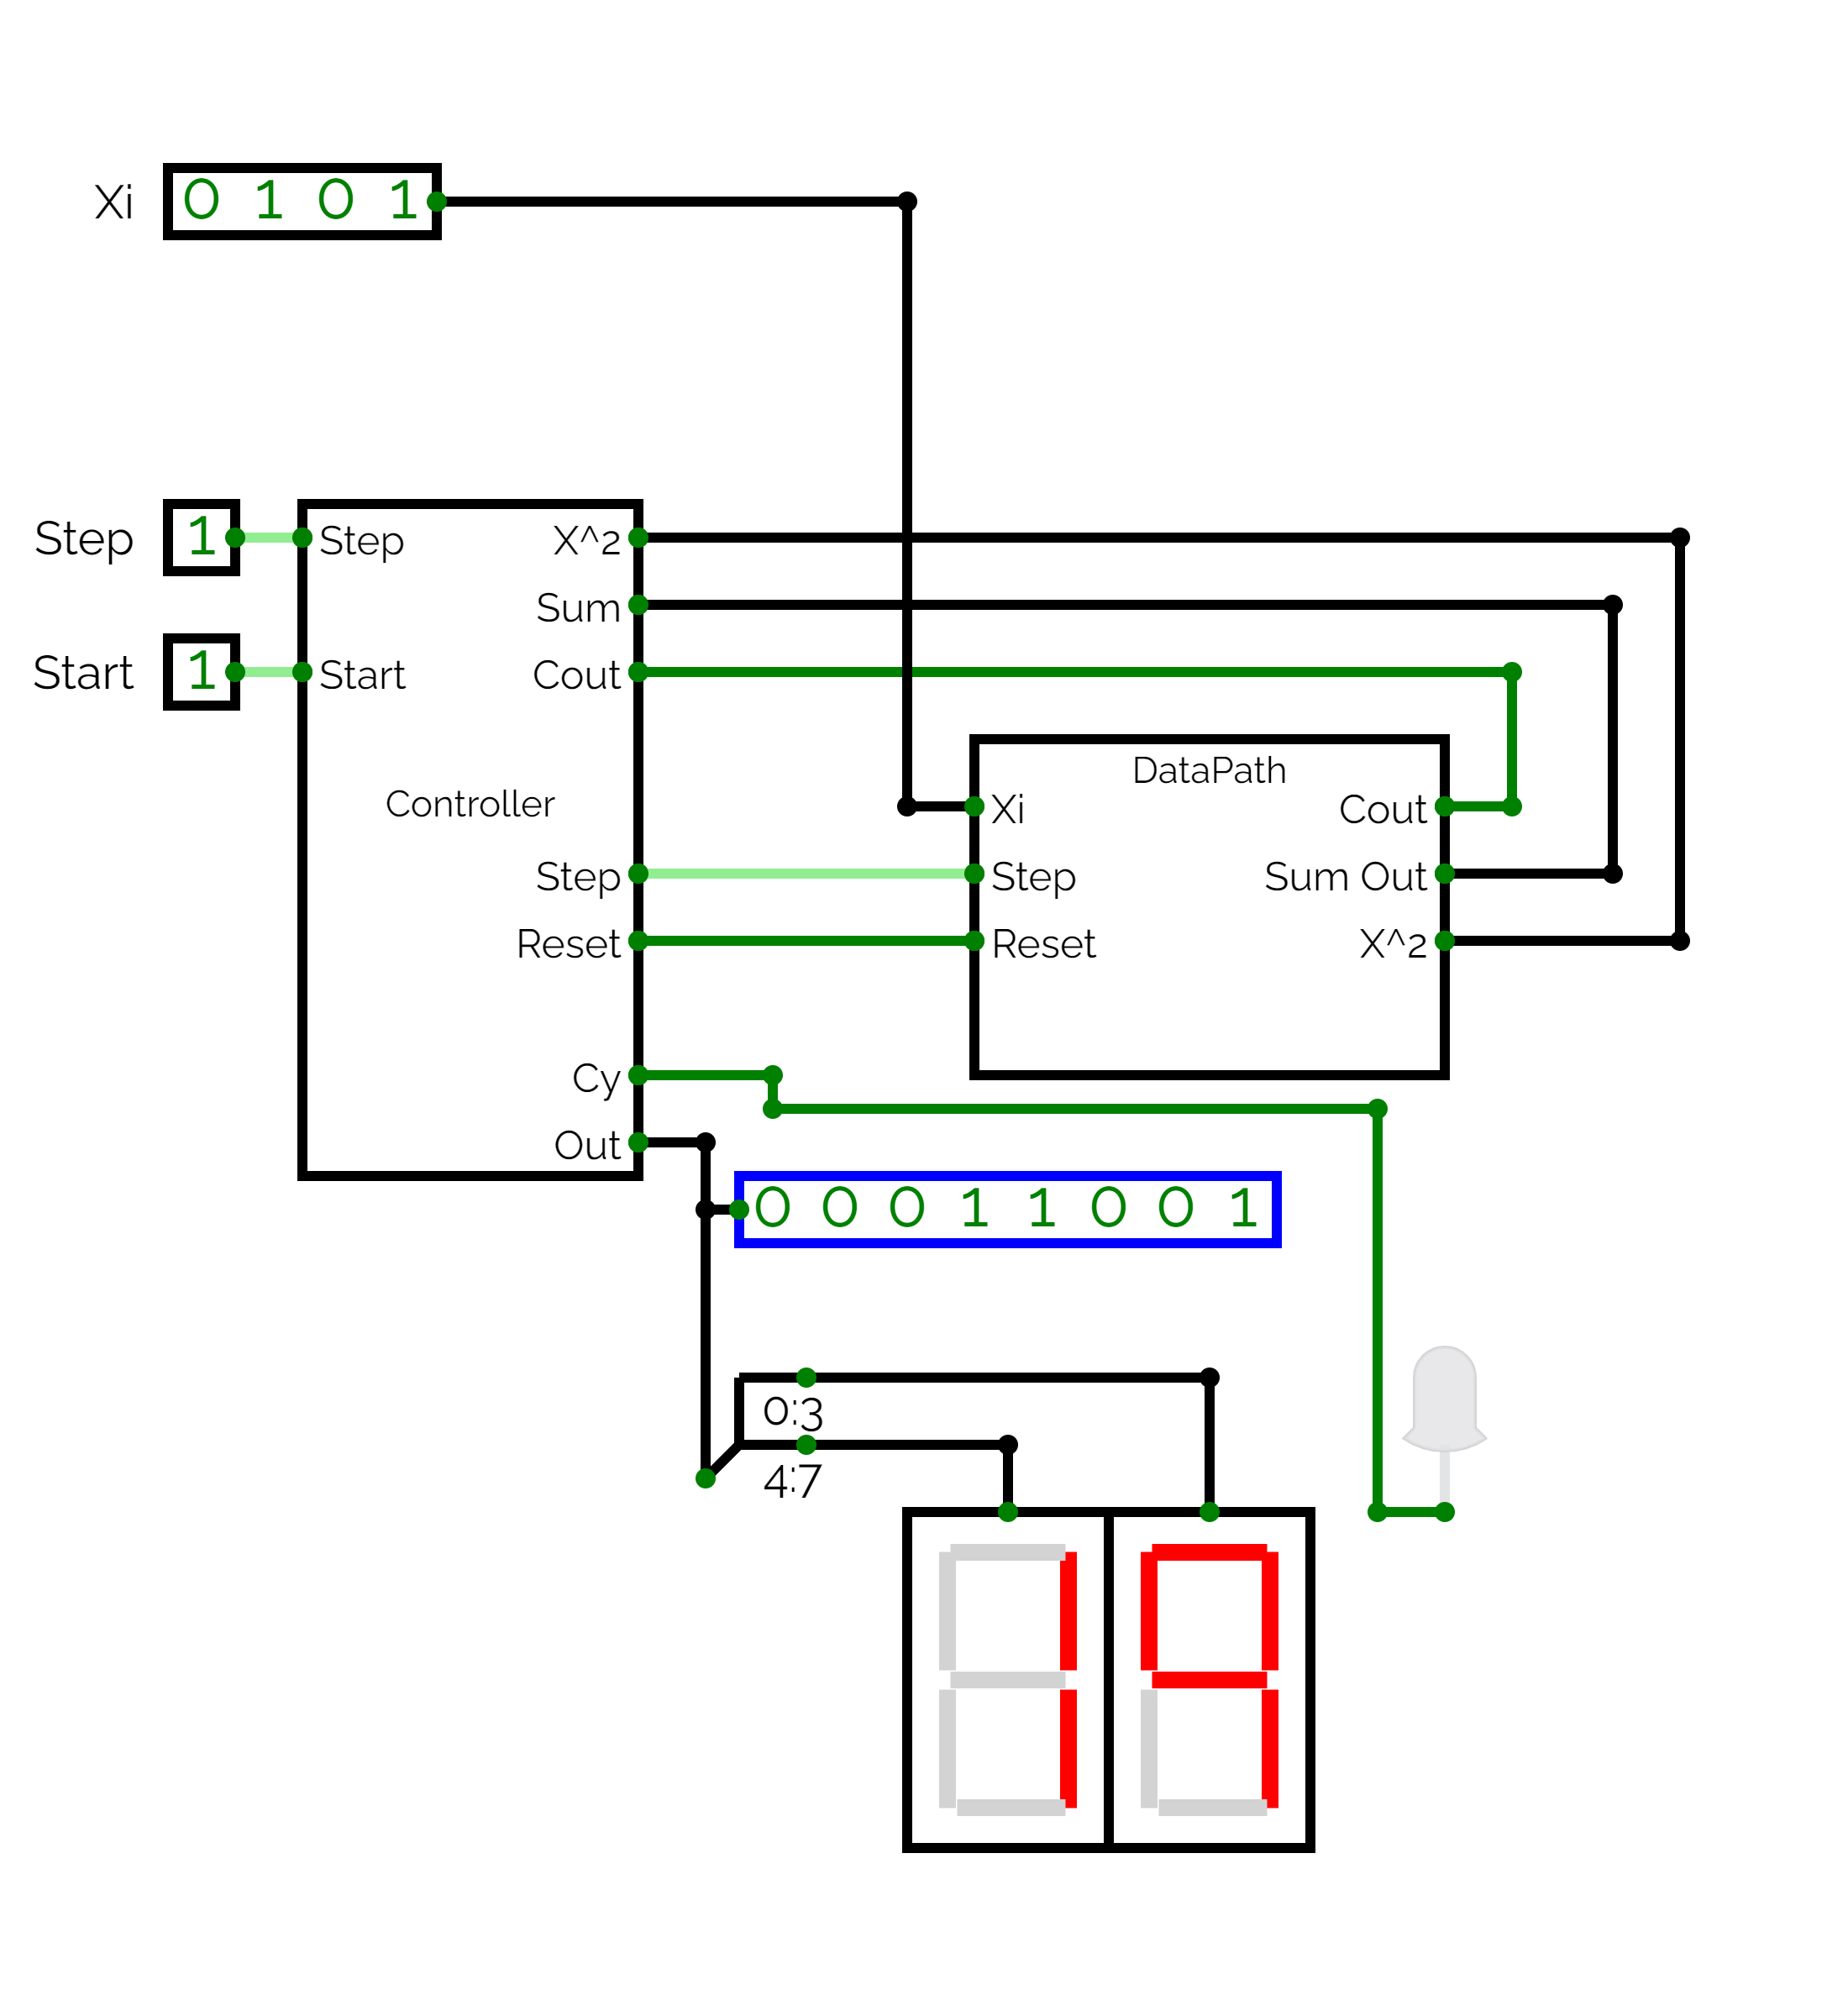
\includegraphics[scale=.08]{Montagem Laboratorial/images/Main (3).png}
        \caption{Teste no \textit{CircuitVerse} (2)}\label{fig:CV2}
    \end{figure}
\end{multicols}

\begin{multicols}{2}
    \begin{figure}[H]
        \centering
        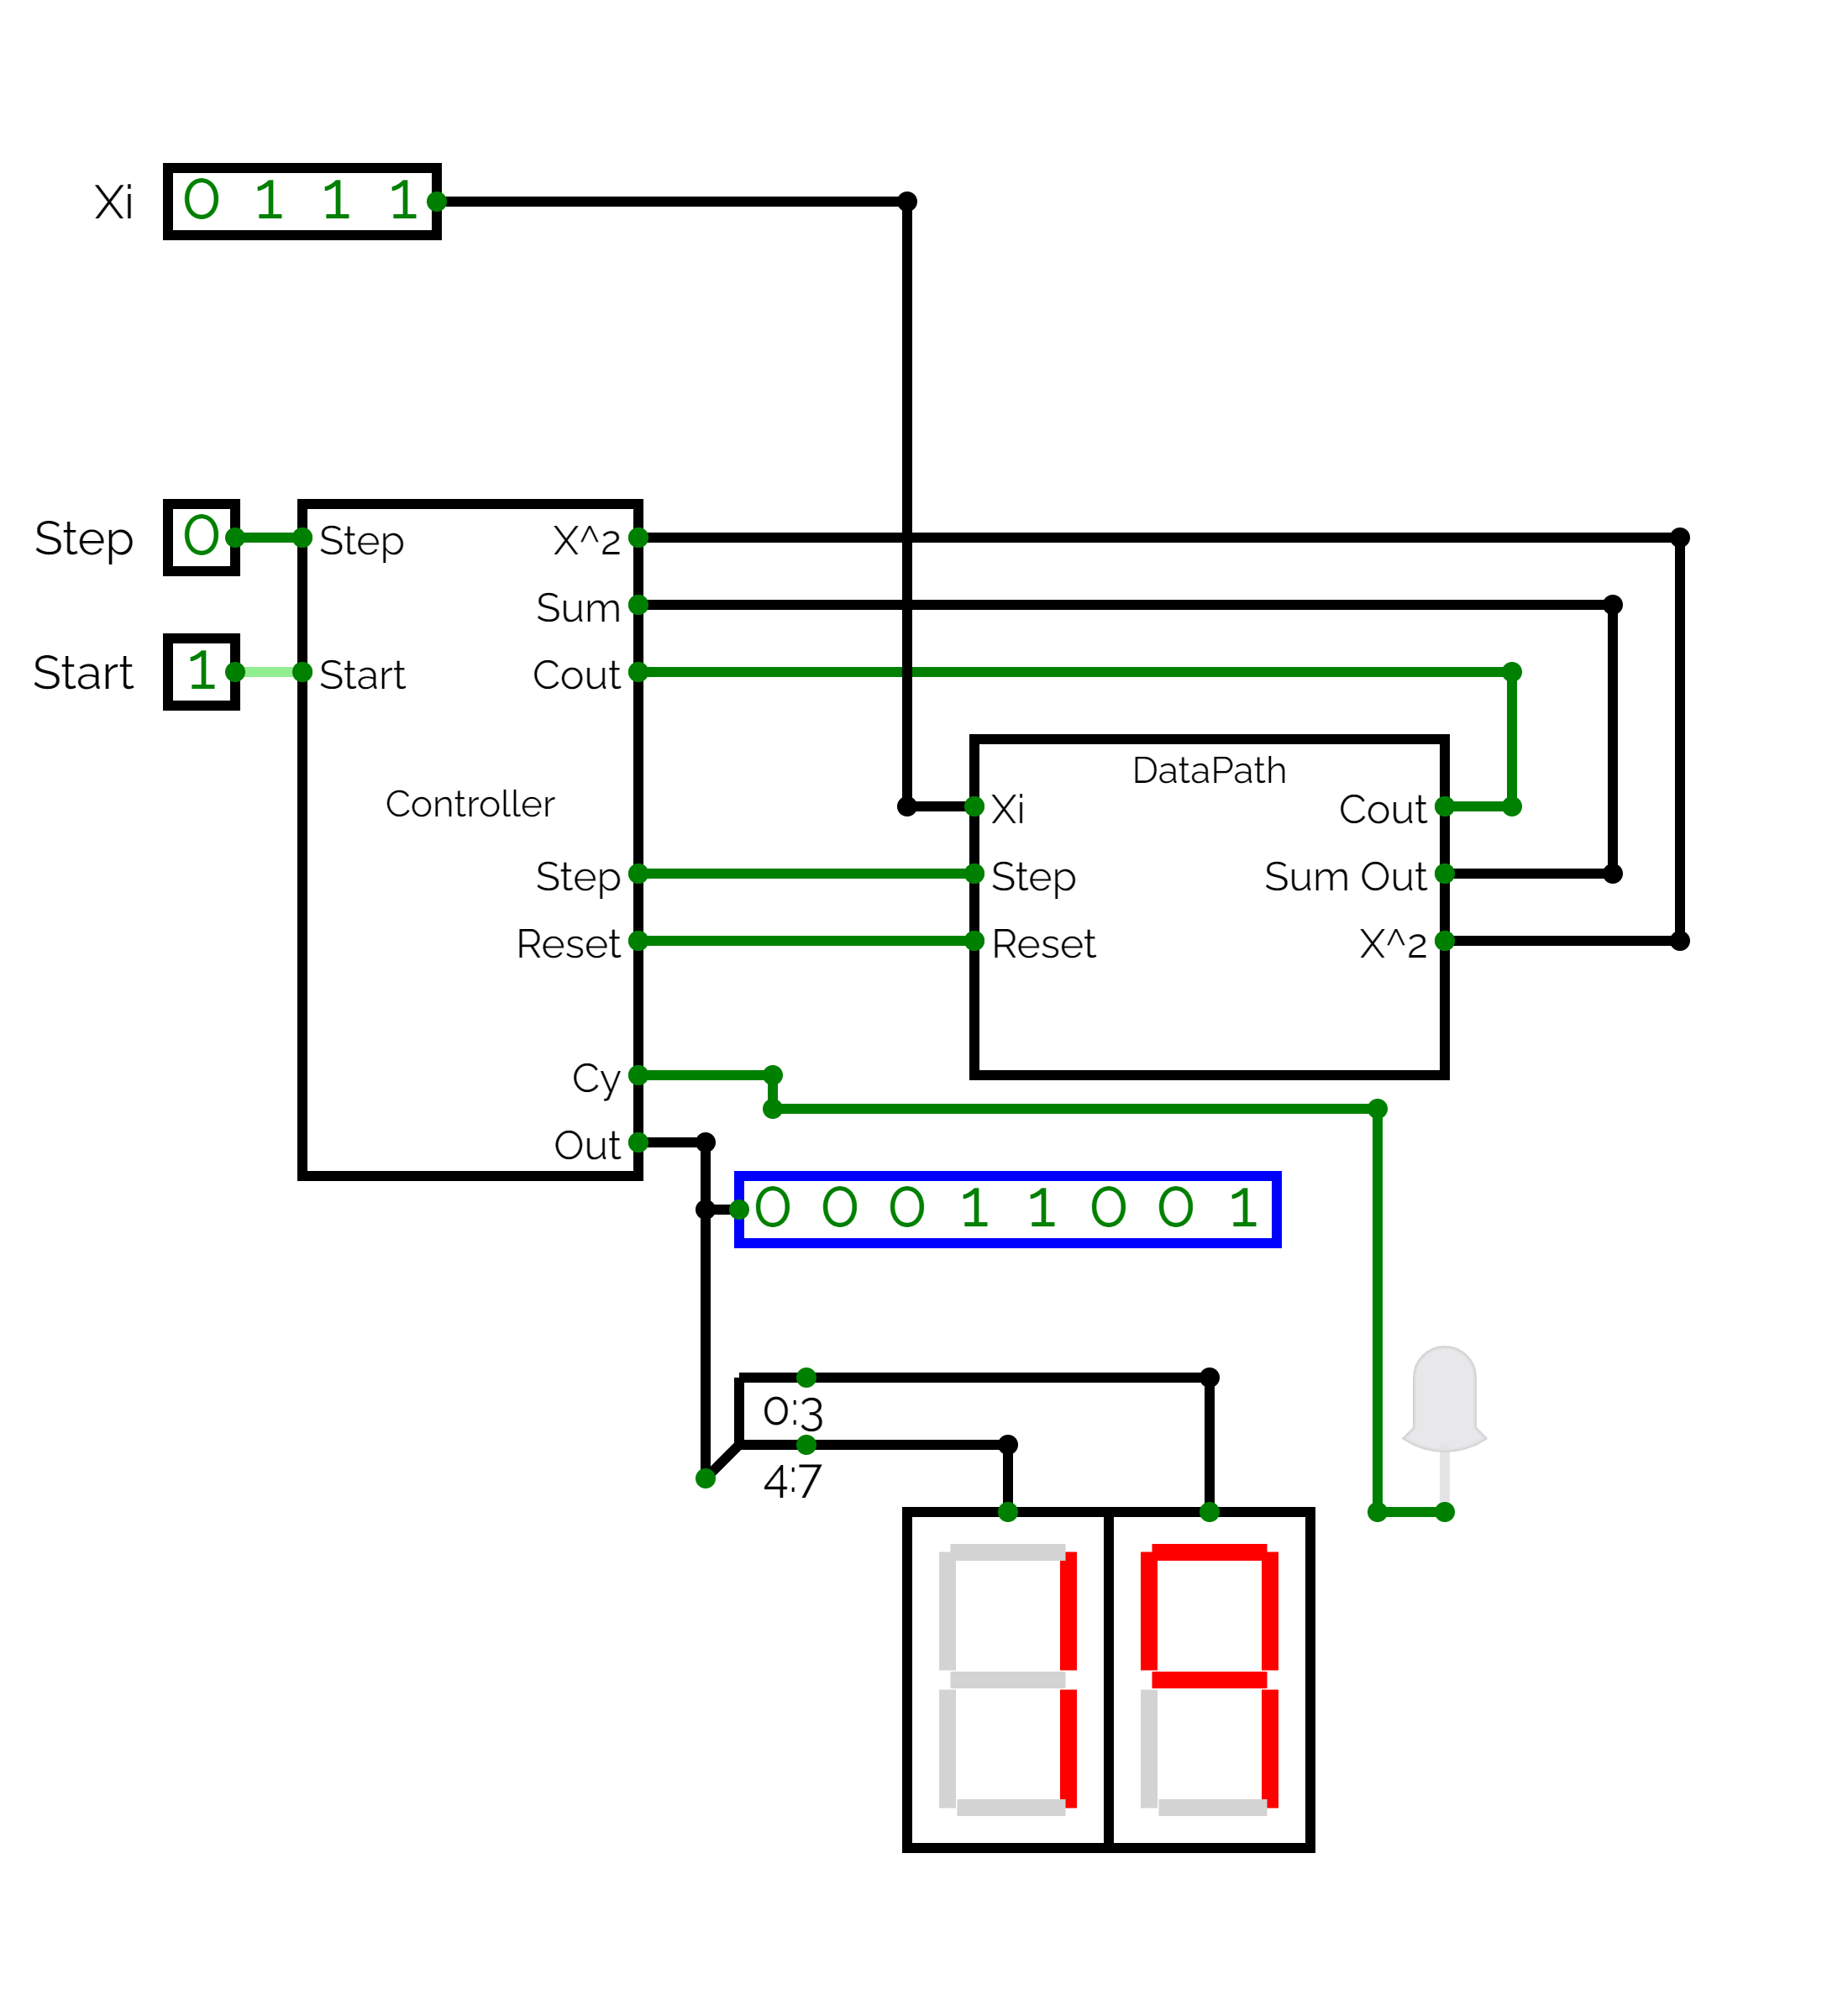
\includegraphics[scale=.08]{Montagem Laboratorial/images/Main (5).png}
        \caption{Teste no \textit{CircuitVerse} (3)}\label{fig:CV3}
    \end{figure}
    \begin{figure}[H]
        \centering
        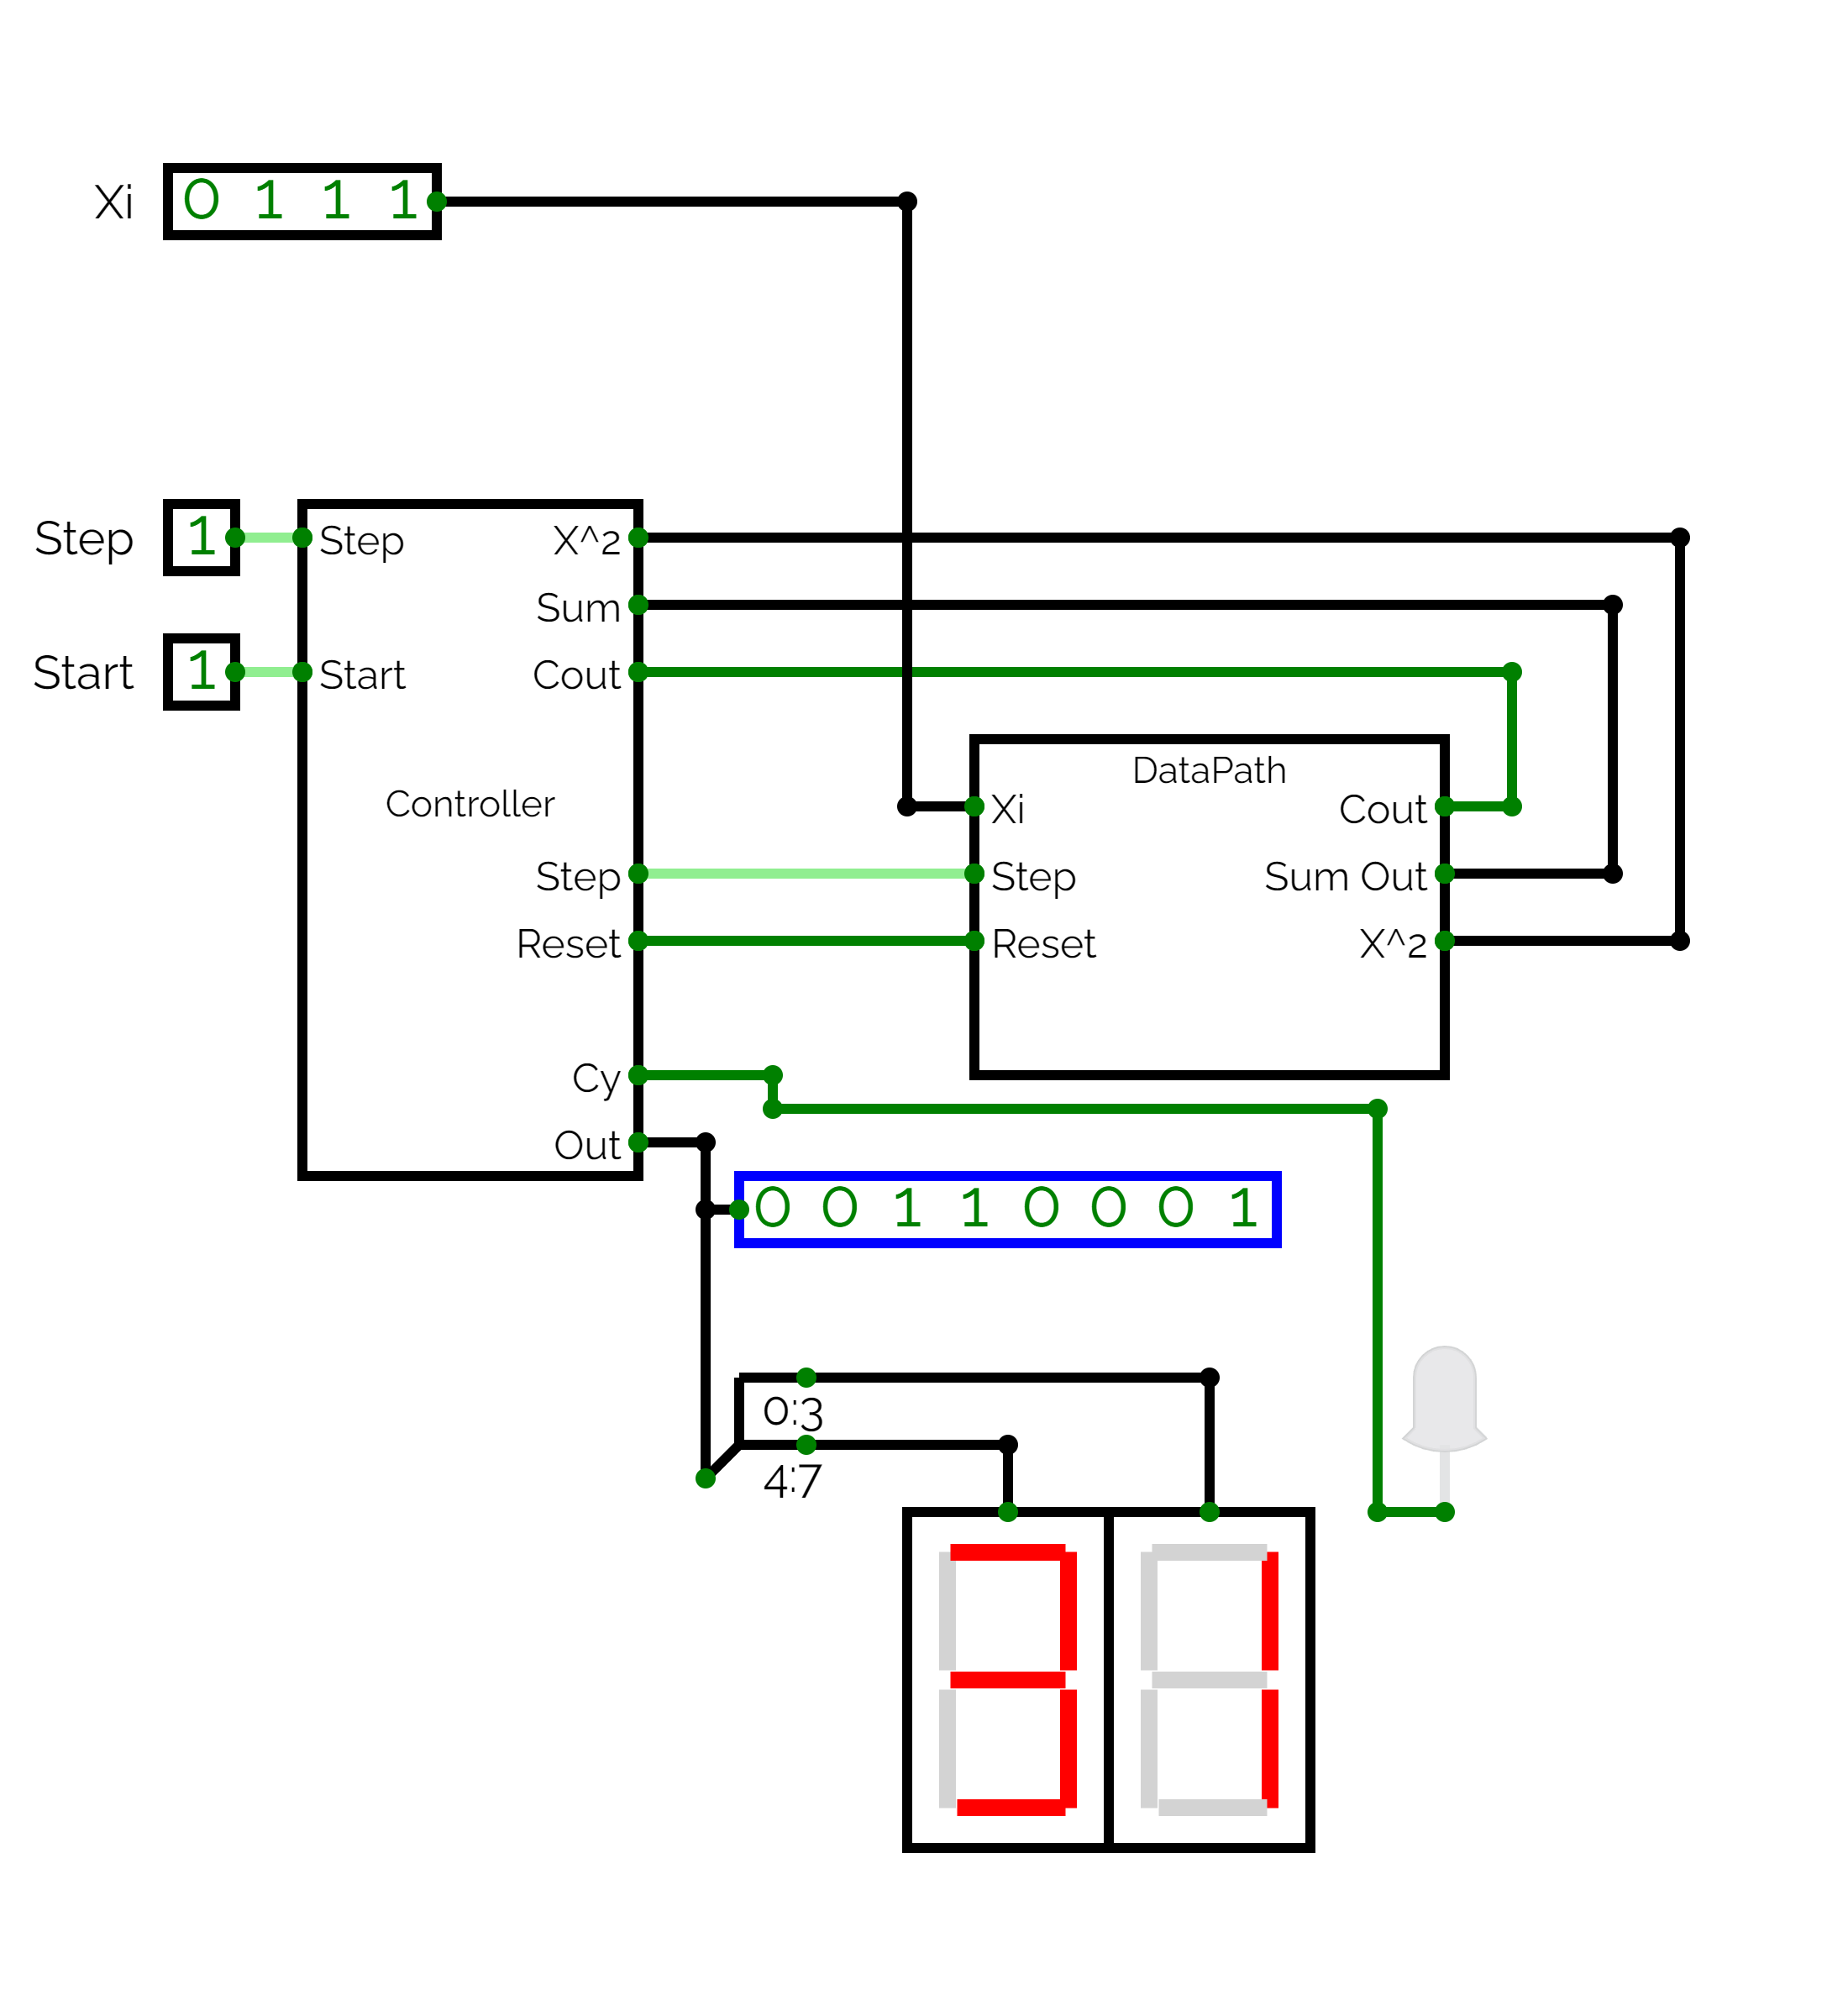
\includegraphics[scale=.08]{Montagem Laboratorial/images/Main (6).png}
        \caption{Teste no \textit{CircuitVerse} (4)}\label{fig:CV4}
    \end{figure}
\end{multicols}

\begin{multicols}{2}
    \begin{figure}[H]
        \centering
        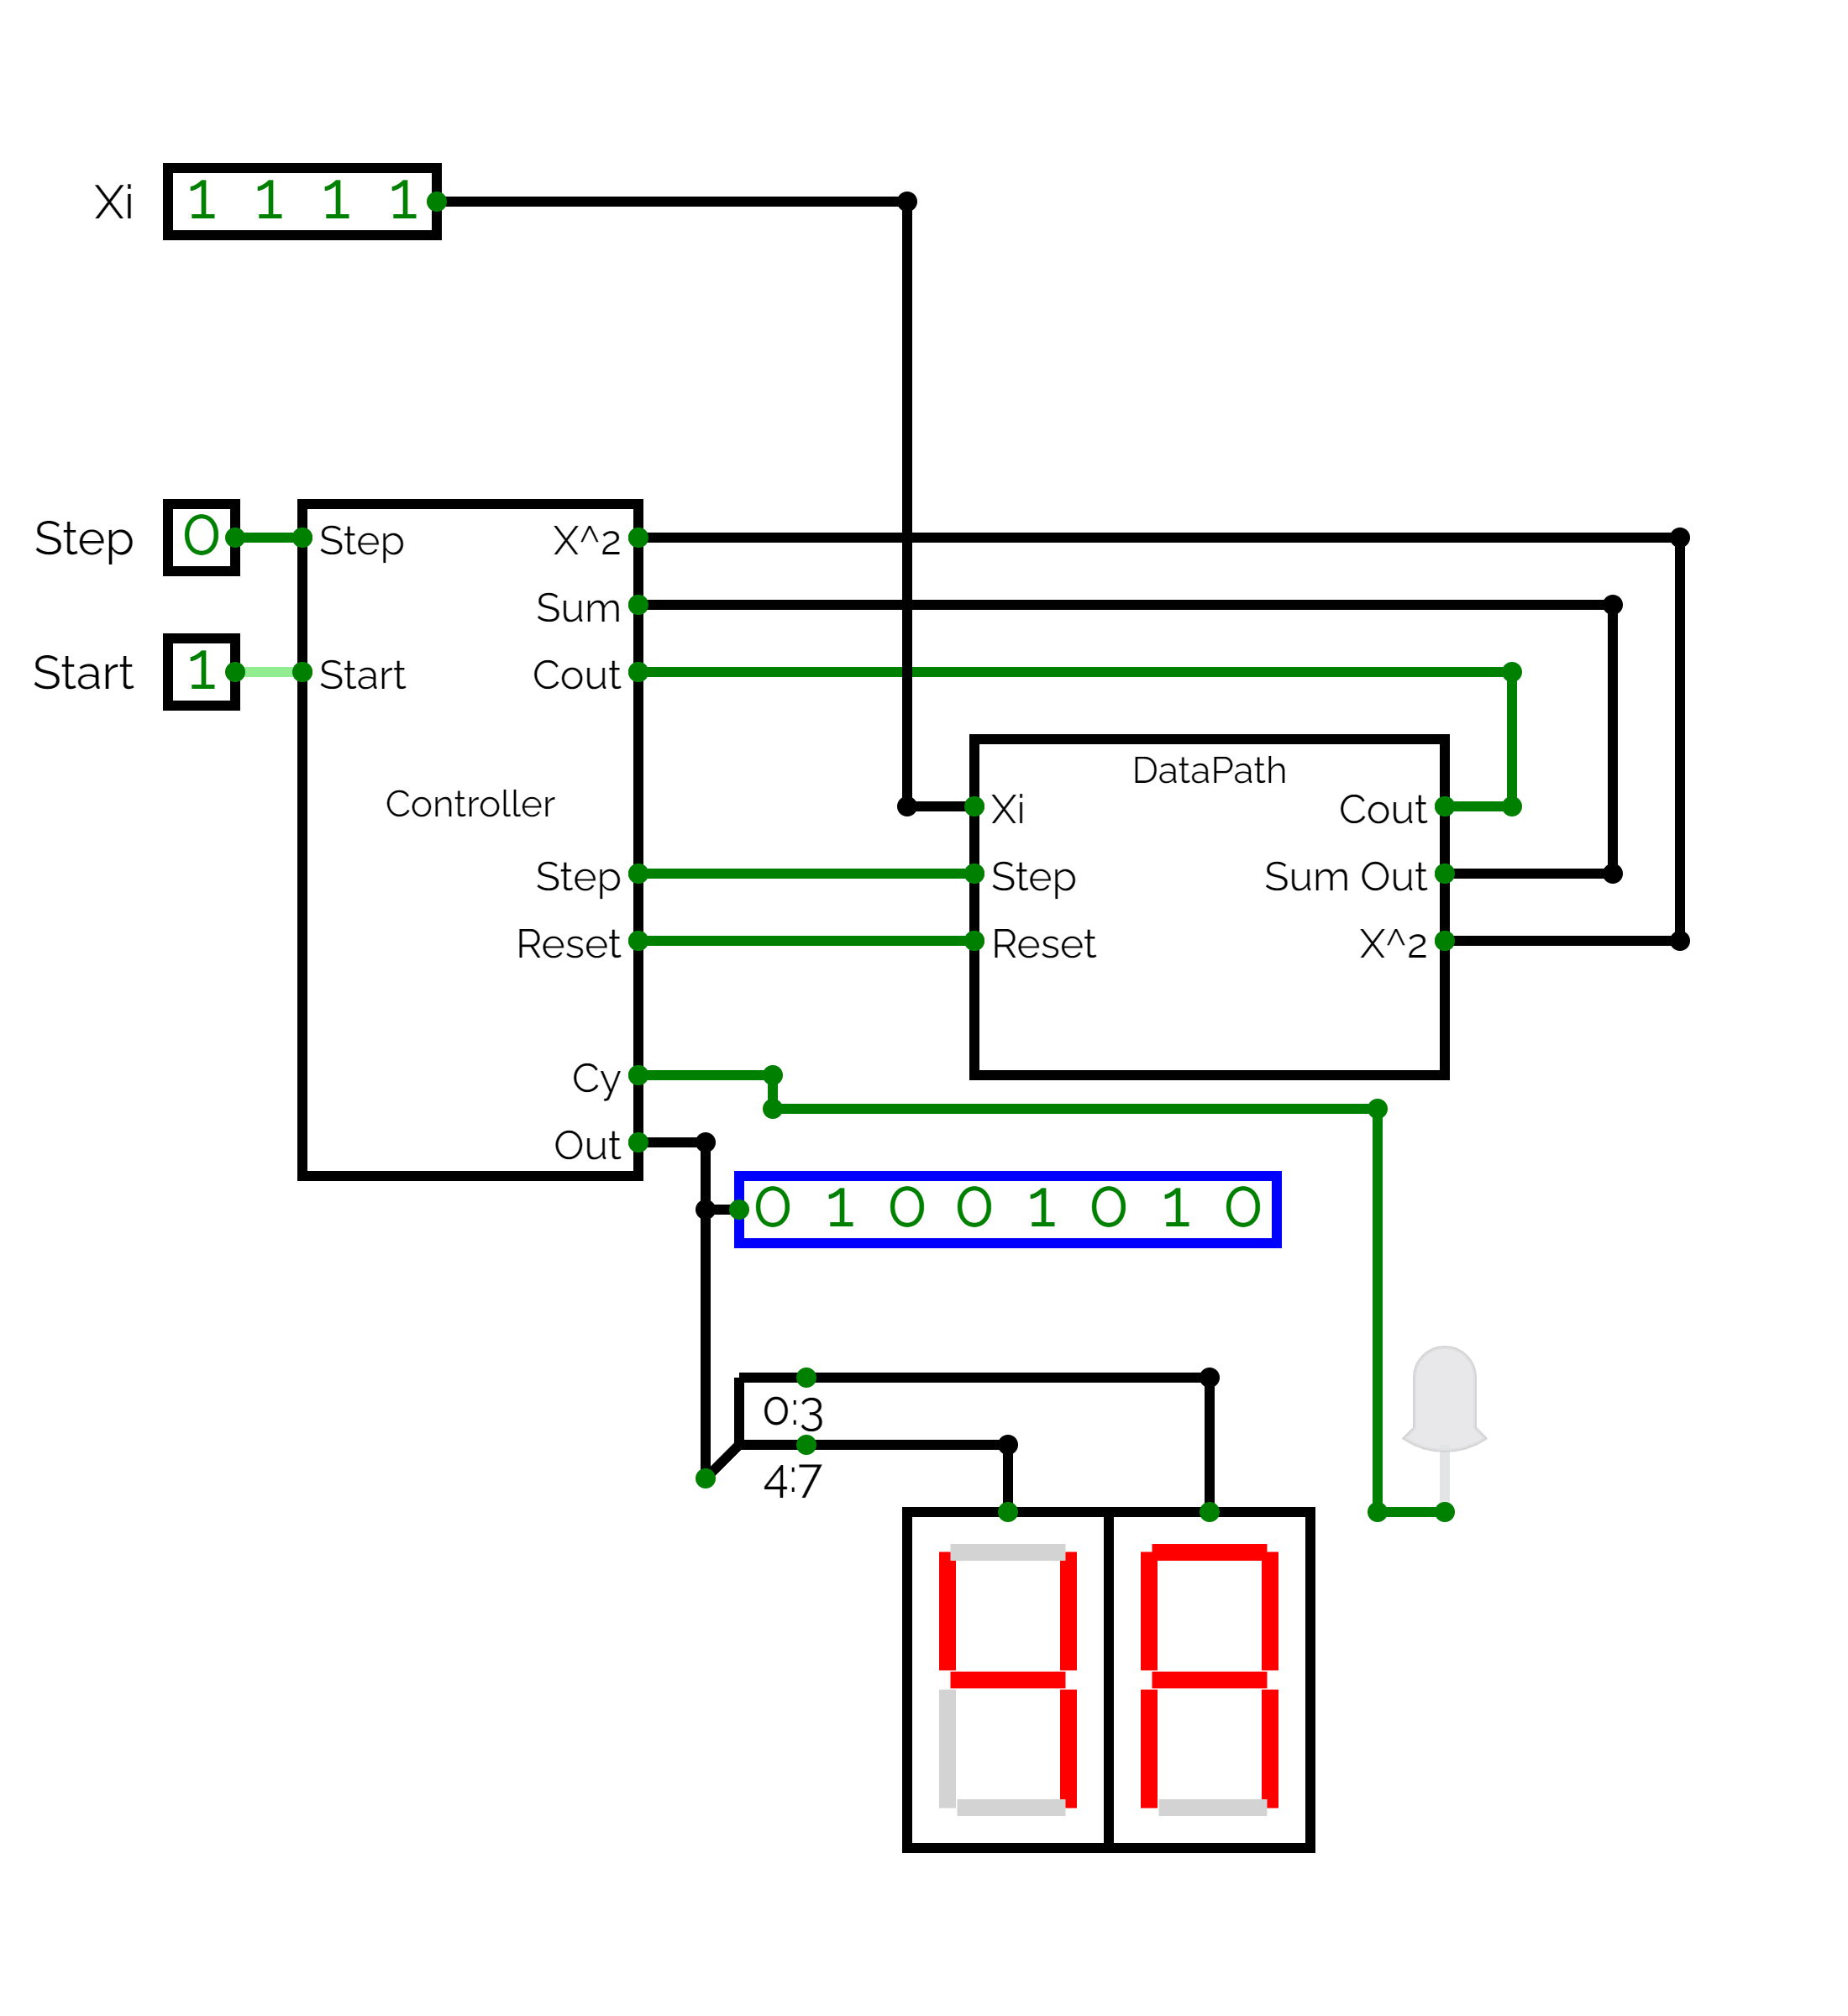
\includegraphics[scale=.08]{Montagem Laboratorial/images/Main (8).png}
        \caption{Teste no \textit{CircuitVerse} (5)}\label{fig:CV5}
    \end{figure}
    \begin{figure}[H]
        \centering
        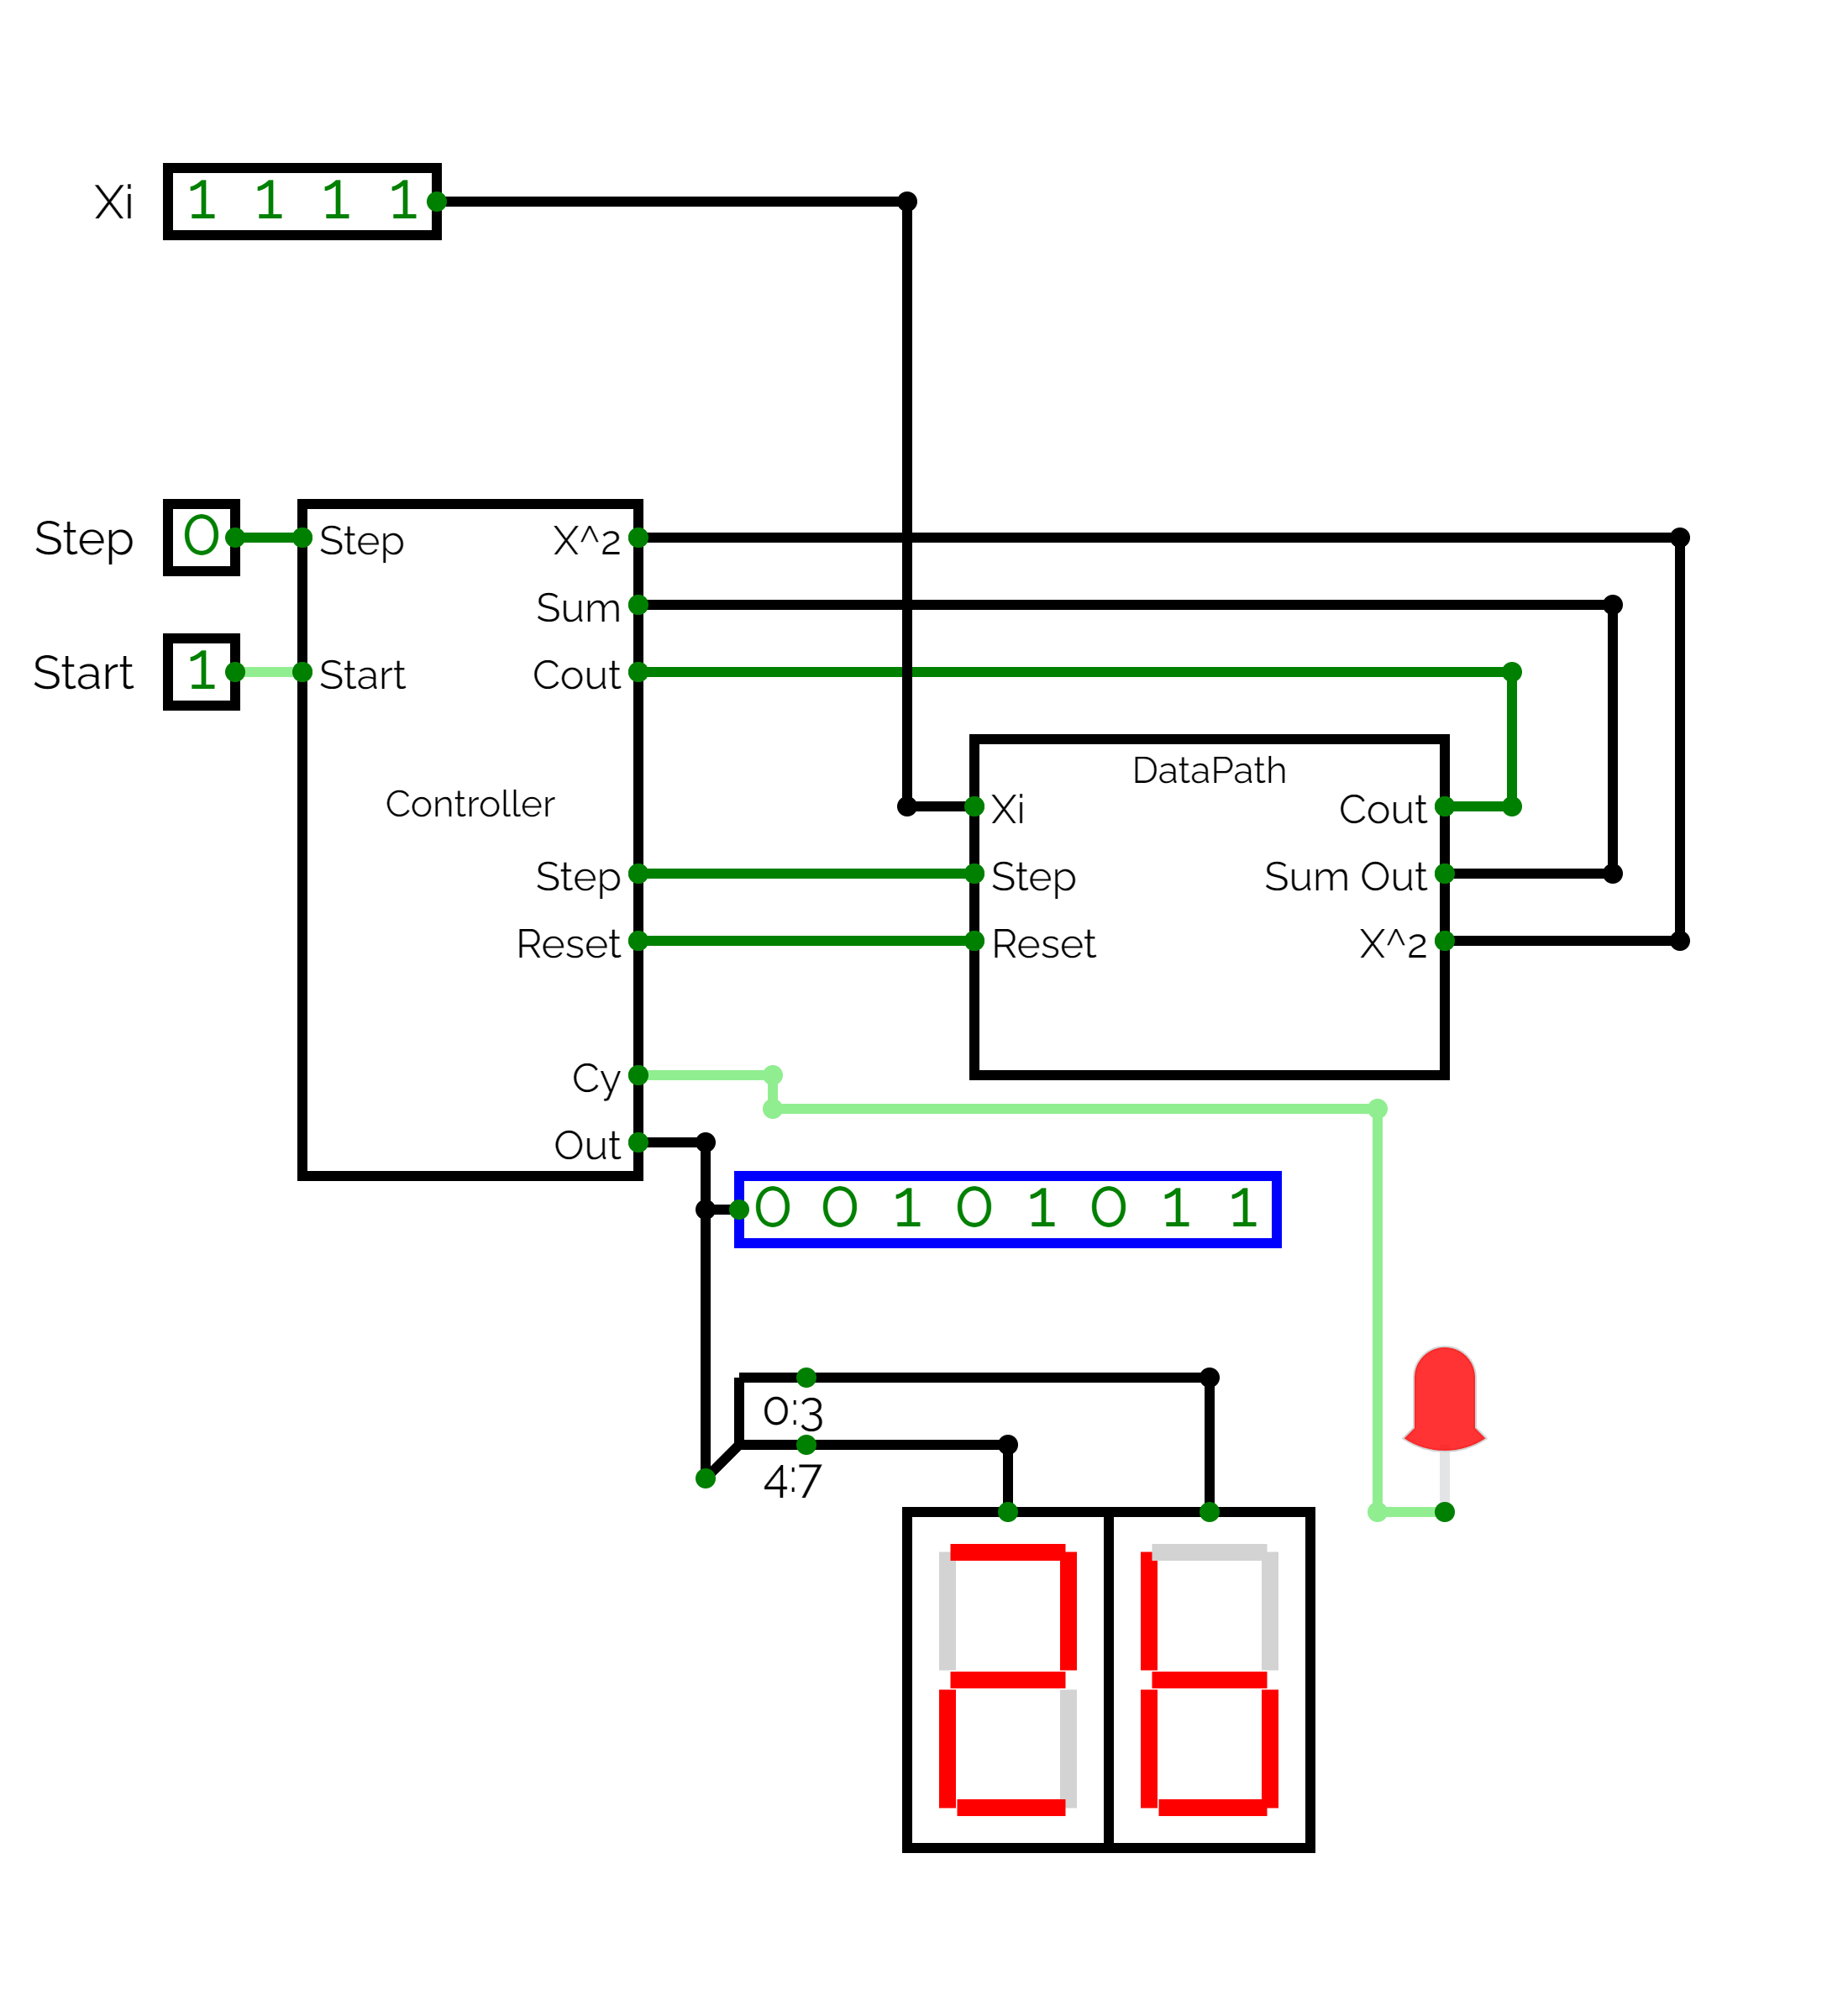
\includegraphics[scale=.08]{Montagem Laboratorial/images/Main (10).png}
        \caption{Teste no \textit{CircuitVerse} (6)}\label{fig:CV6}
    \end{figure}
\end{multicols}

De forma abrangente, a verificação de casos singulares, que englobam todos os cenários possíveis de resposta, sintetiza a comprovação de todas as combinações viáveis. Na figura~\ref{fig:RTLSimulator}, apresentamos algumas combinações testadas no \textit{RTL Simulation}.

\begin{figure}[H]
    \centering
    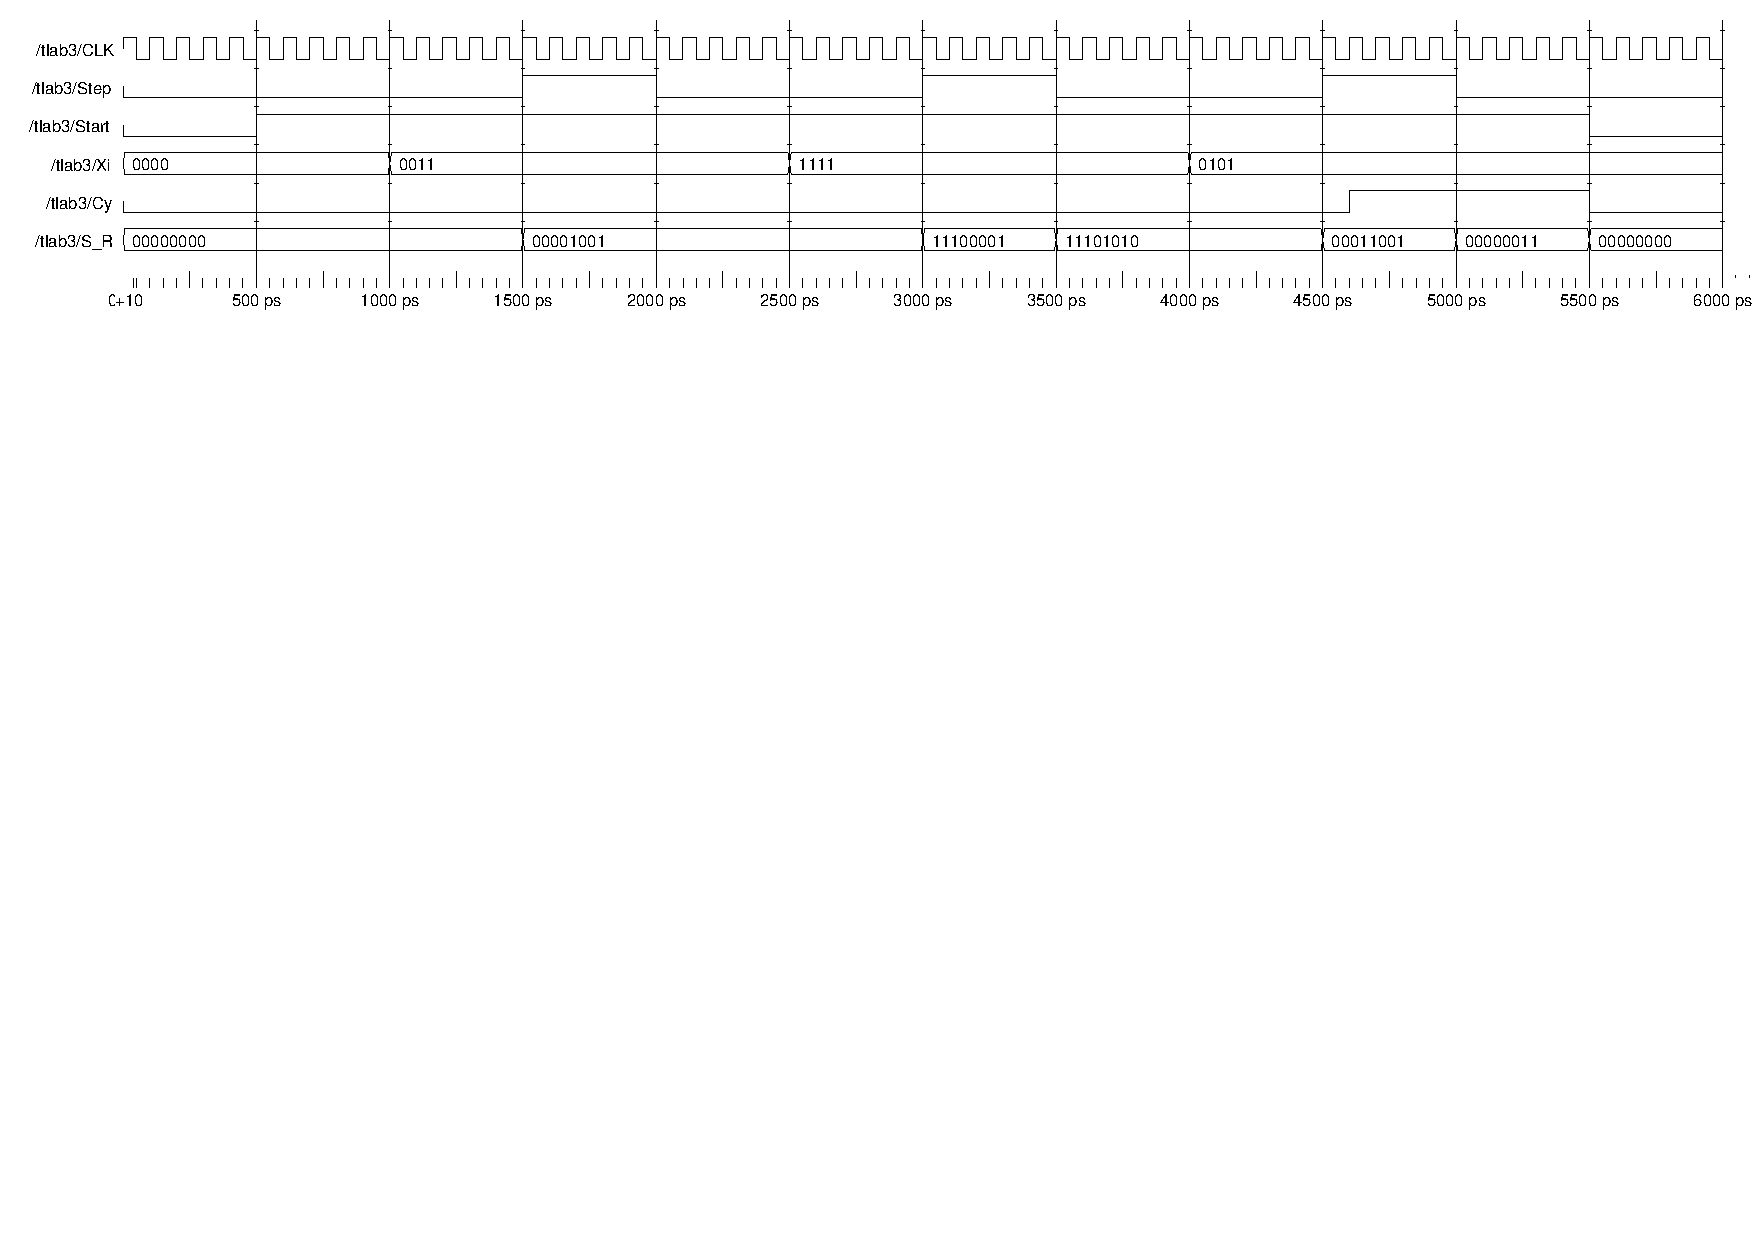
\includegraphics[trim={0 15cm 0 0},clip,width=\linewidth]{Montagem Laboratorial/images/RTLSim1.pdf}
    \caption{Simulação no \textit{RTL Simulation}}\label{fig:RTLSimulator}
\end{figure}

Como se pode observar na figura acima, inicialmente temos a nossa entrada $x_i$ a 0. De seguida, acionámos o Start a 1, mantendo a entrada $x_i$ a 0. De imediato, forçámos o valor de $x_i$ a 3 $(0011)$, e ligámos a entrada Step logo de seguida. Observámos o valor do quadrado de 3 $(00001001 = 9)$, confirmando a funcionalidade do módulo responsável pelo cálculo do quadrado. Ao desligar o Step, continua o valor de 9 a ser mostrado.

Novamente introduzindo um novo valor de $x_i$, neste caso optámos pelo 15 $(1111)$, e ligámos de seguida a entrada Step, verificamos que o valor que surge no final é, definitivamente, o quadrado de 15 $(11100001 = 225)$.

No ato de desligar o Step, agora o valor que surge é a soma dos quadrados já realizados até então, que neste caso origina o valor de 234 $(00001001 (9) + 11100001 (225) = 11101010 (234))$.

Definimos mais uma vez um novo valor para $x_i$, que neste caso, será o 5 $(0101)$, e ligámos a entrada Step. Notámos que ao ligar o Step, o output Cy ativou-se, o que indica que o número que irá ser representado após o Step passar a 0, não pode ser representado pelos 8 bits, que é o limite de bits para este trabalho.

Por outras palavras, o Cy ativa-se logo de imediato porque, nesse preciso momento que ativamos o Step, o valor acumulado dos quadrados já excedeu o limite definido. Observa-se o valor do quadrado de 5 $(00011001 = 25)$ e ao desativar a entrada Step, observa-se o valor de 3 $(00000011 = 3)$, isto porque, o acumulador, neste momento, porta o valor de 259 $(9 + 225 + 25)$, que excede o limite dos números naturais que podem ser representados por 8 bits (0 ao 255).

Por esse motivo, o resultado apresentado é a diferença que não pode ser representada corretamente. Diante disso, consideramos que quando o número alcança o valor 255, ele recomeça a contagem do zero, daí resulta o resultado 3 $(00000011)$ indicado no final.
Por fim, desativámos a entrada Start, no que resultou num Reset ao circuito, que retornou o valor da saída a 0.

\subsection{Resultados Experimentais e Validação na Placa}

Neste tópico, apresentam-se os resultados obtidos a partir da implementação do circuito projetado para calcular o quadrado de números naturais. O objetivo principal foi verificar a funcionalidade e a precisão do circuito em diferentes condições de operação, avaliando seu desempenho com diversos valores de entrada. Os dados recolhidos foram analisados e comparados com os valores teóricos esperados, a fim de validar a conformidade entre a resposta prática — em simulação e na placa — e os valores teóricos previamente estabelecidos.

Como a função deste circuito é calcular o quadrado de um número natural de 4 bits, os resultados esperados podem ser facilmente deduzidos.

\subsubsection{Validação na Placa}

Com o circuito devidamente carregado na placa, realizamos os testes desejados. Após várias combinações nos \textit{switches} da placa e observando as reações nos \textit{displays} de 7 segmentos, foi possível confirmar que o objetivo do trabalho foi alcançado corretamente.

Verificamos que os quadrados gerados a partir dos inputs introduzidos nos \textit{switches} eram exibidos conforme esperado, comprovando que o circuito executava exatamente o que foi estipulado no enunciado do trabalho. Nas figuras abaixo, demonstramos uma série de testes realizados na placa.
\vspace*{\fill}
\begin{infoclean}
    Note que os dois primeiros interruptores, a contar da esquerda, representam o Start e o Step, respetivamente. Os quatro últimos, representam o valor de $x$.
\end{infoclean}

\begin{multicols}{2}
    \begin{figure}[H]
        \centering
        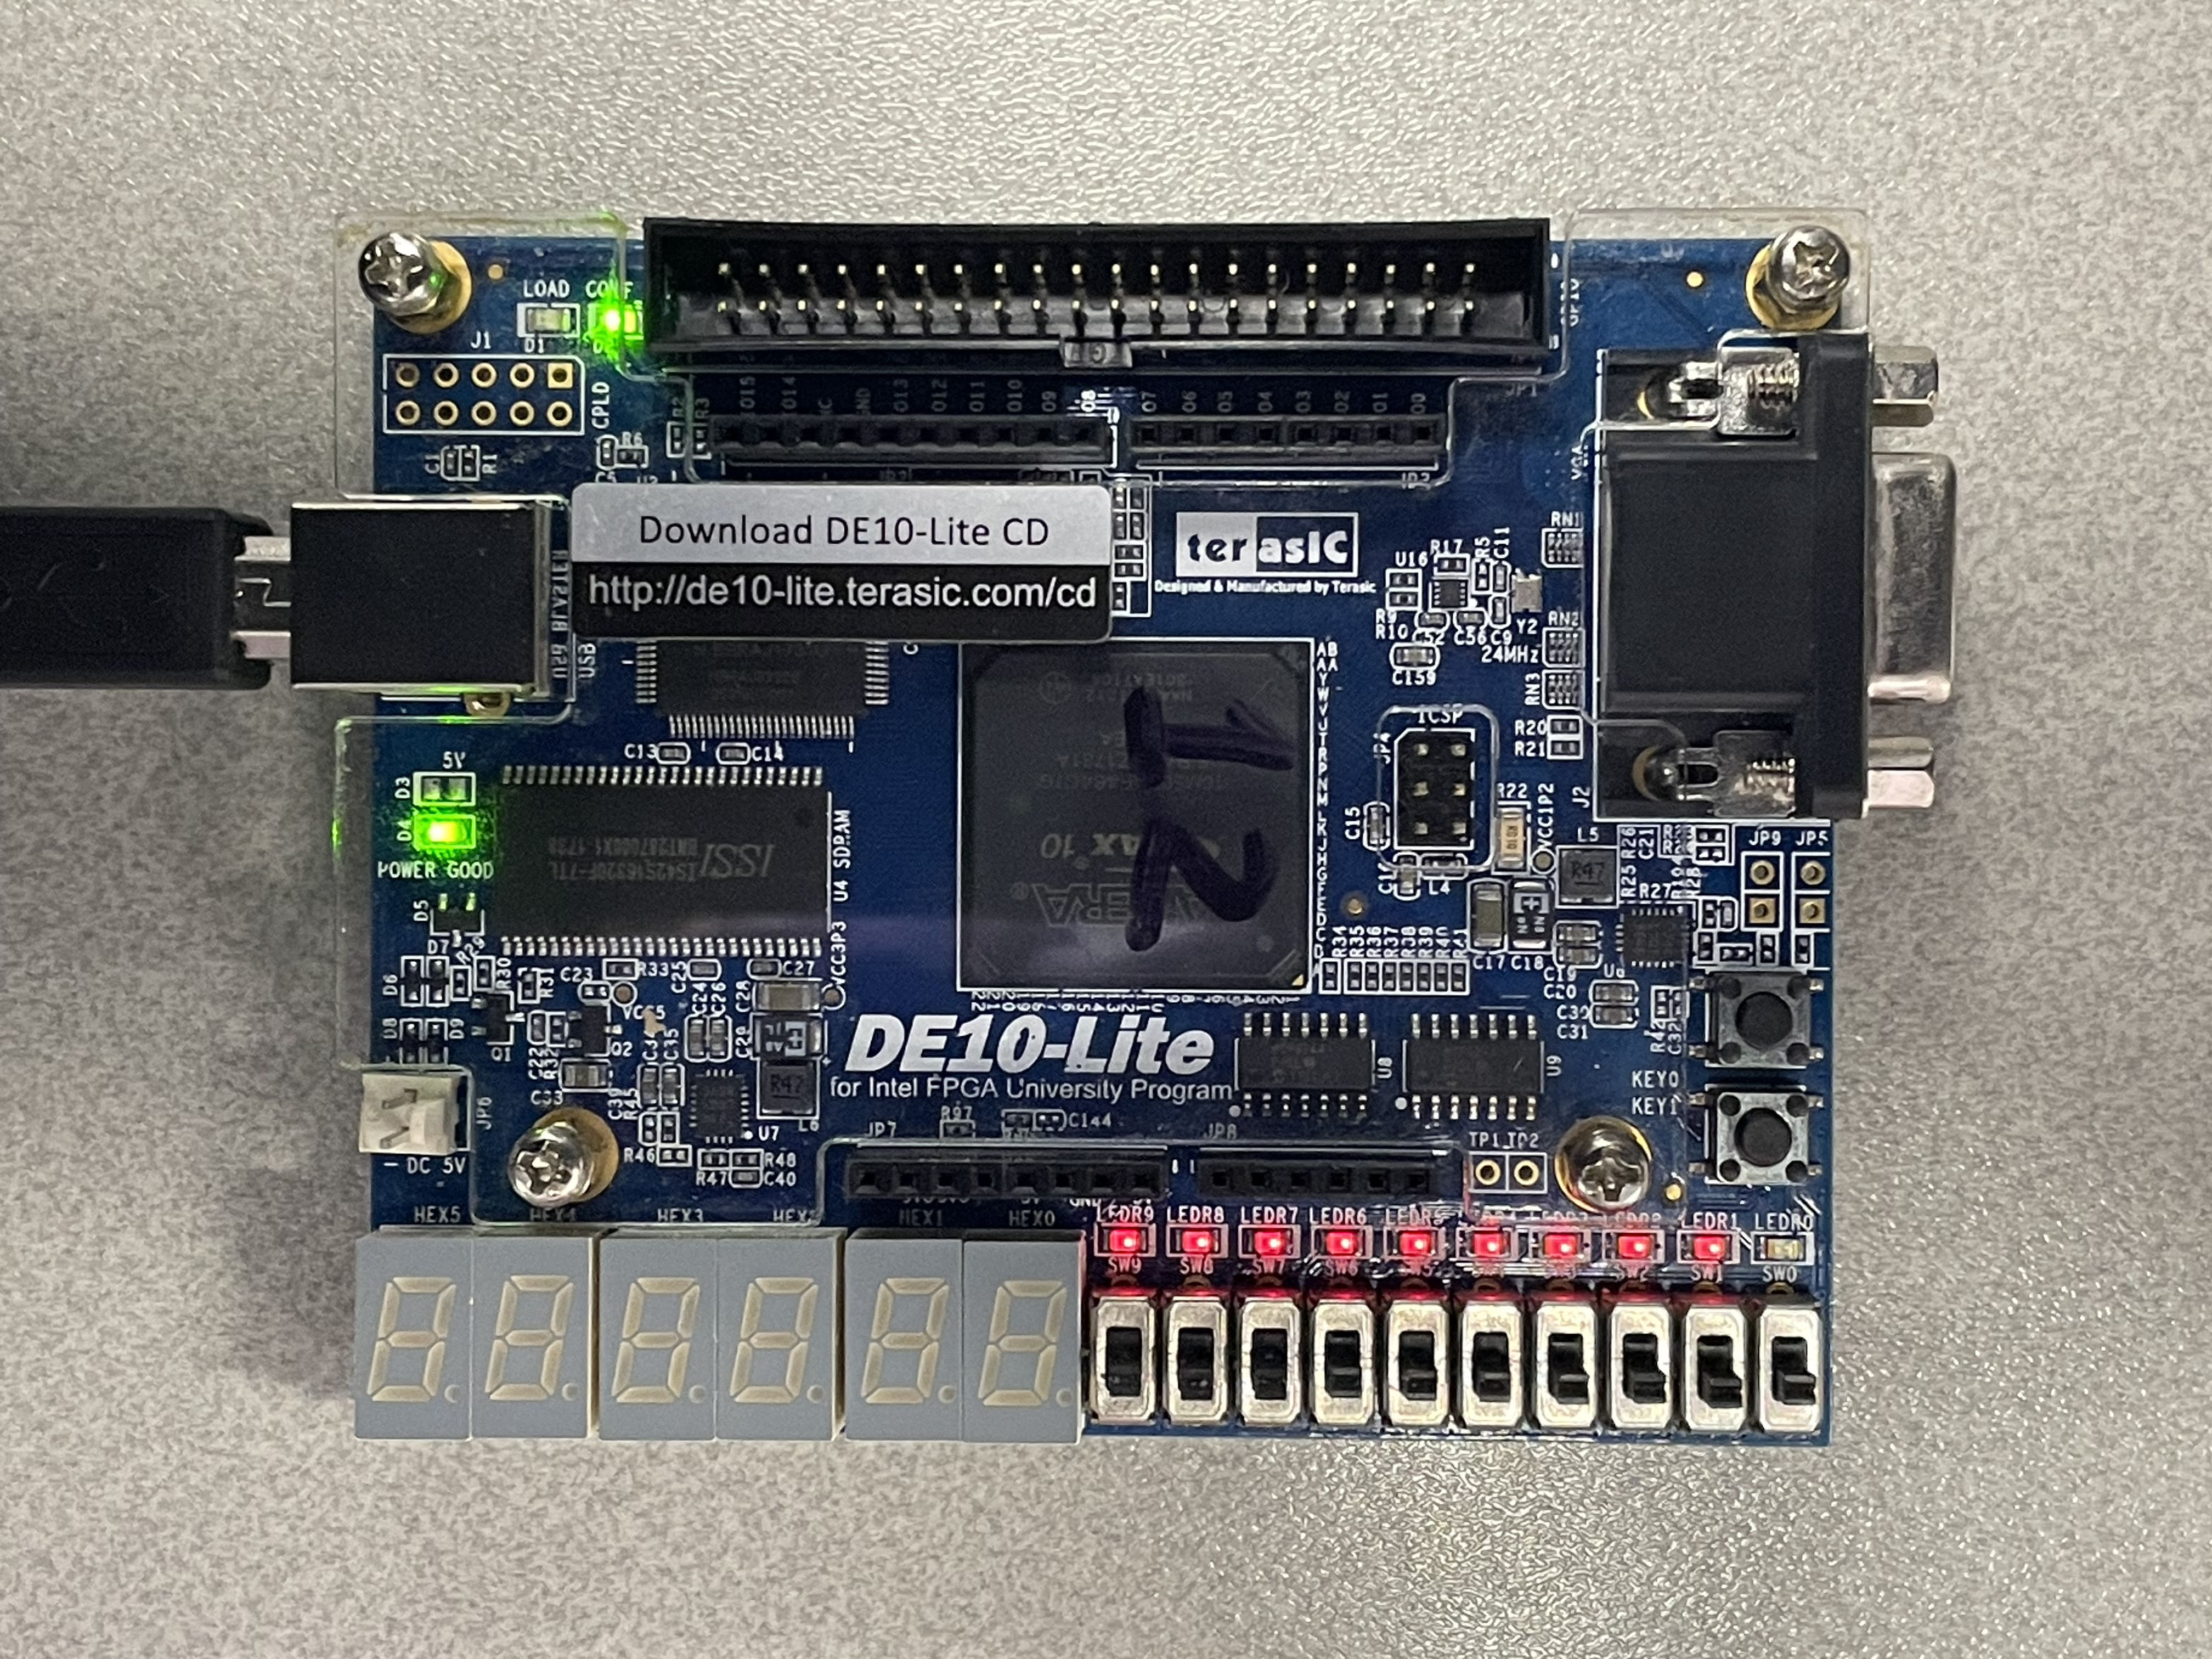
\includegraphics[width=.85\linewidth]{Montagem Laboratorial/images/IMG_2301.png}
        \caption{Teste na DE10-Lite (1)}\label{fig:DE1}
    \end{figure}
    \begin{figure}[H]
        \centering
        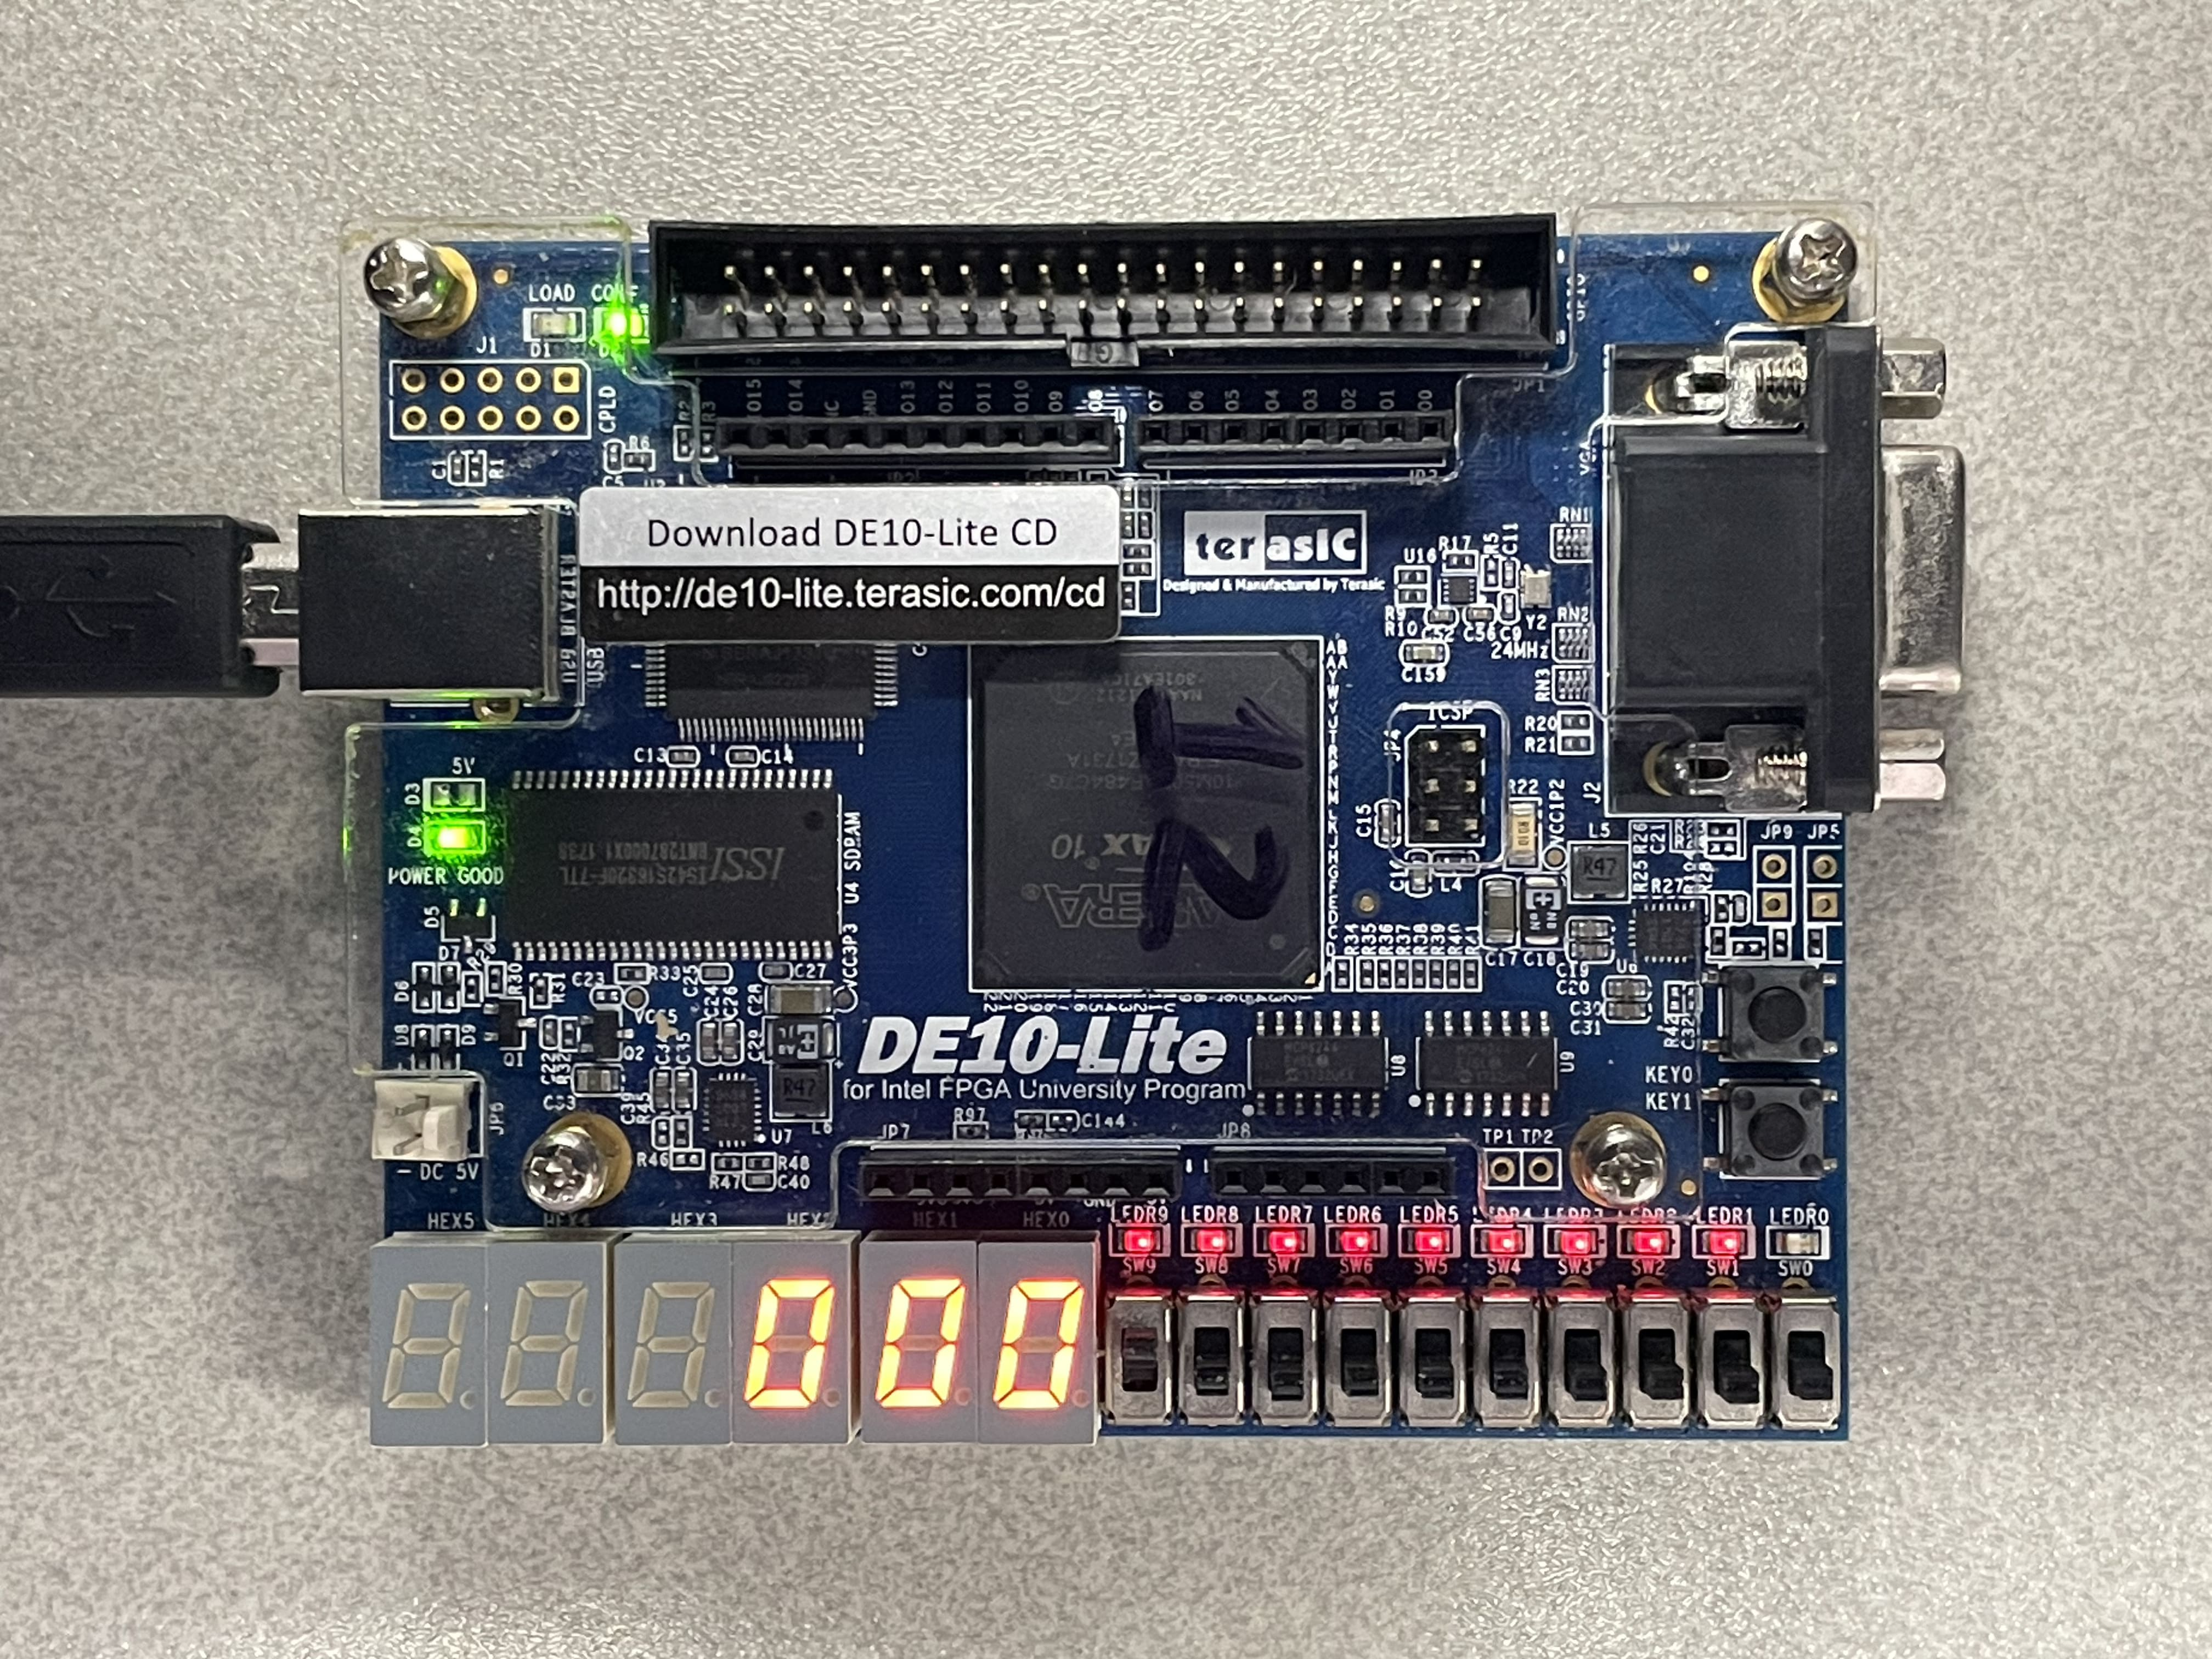
\includegraphics[width=.85\linewidth]{Montagem Laboratorial/images/IMG_2302.png}
        \caption{Teste na DE10-Lite (2)}\label{fig:DE2}
    \end{figure}
\end{multicols}

Na figura~\ref{fig:DE1}, observamos que a placa está no seu estado inicial. Neste caso nada acontece e todos os valores permanecem a zero. De seguida, na figura~\ref{fig:DE2}, a entrada Start foi colocada a 1, indicando ao sistema que vamos começar um cálculo.

\begin{multicols}{2}
    \begin{figure}[H]
        \centering
        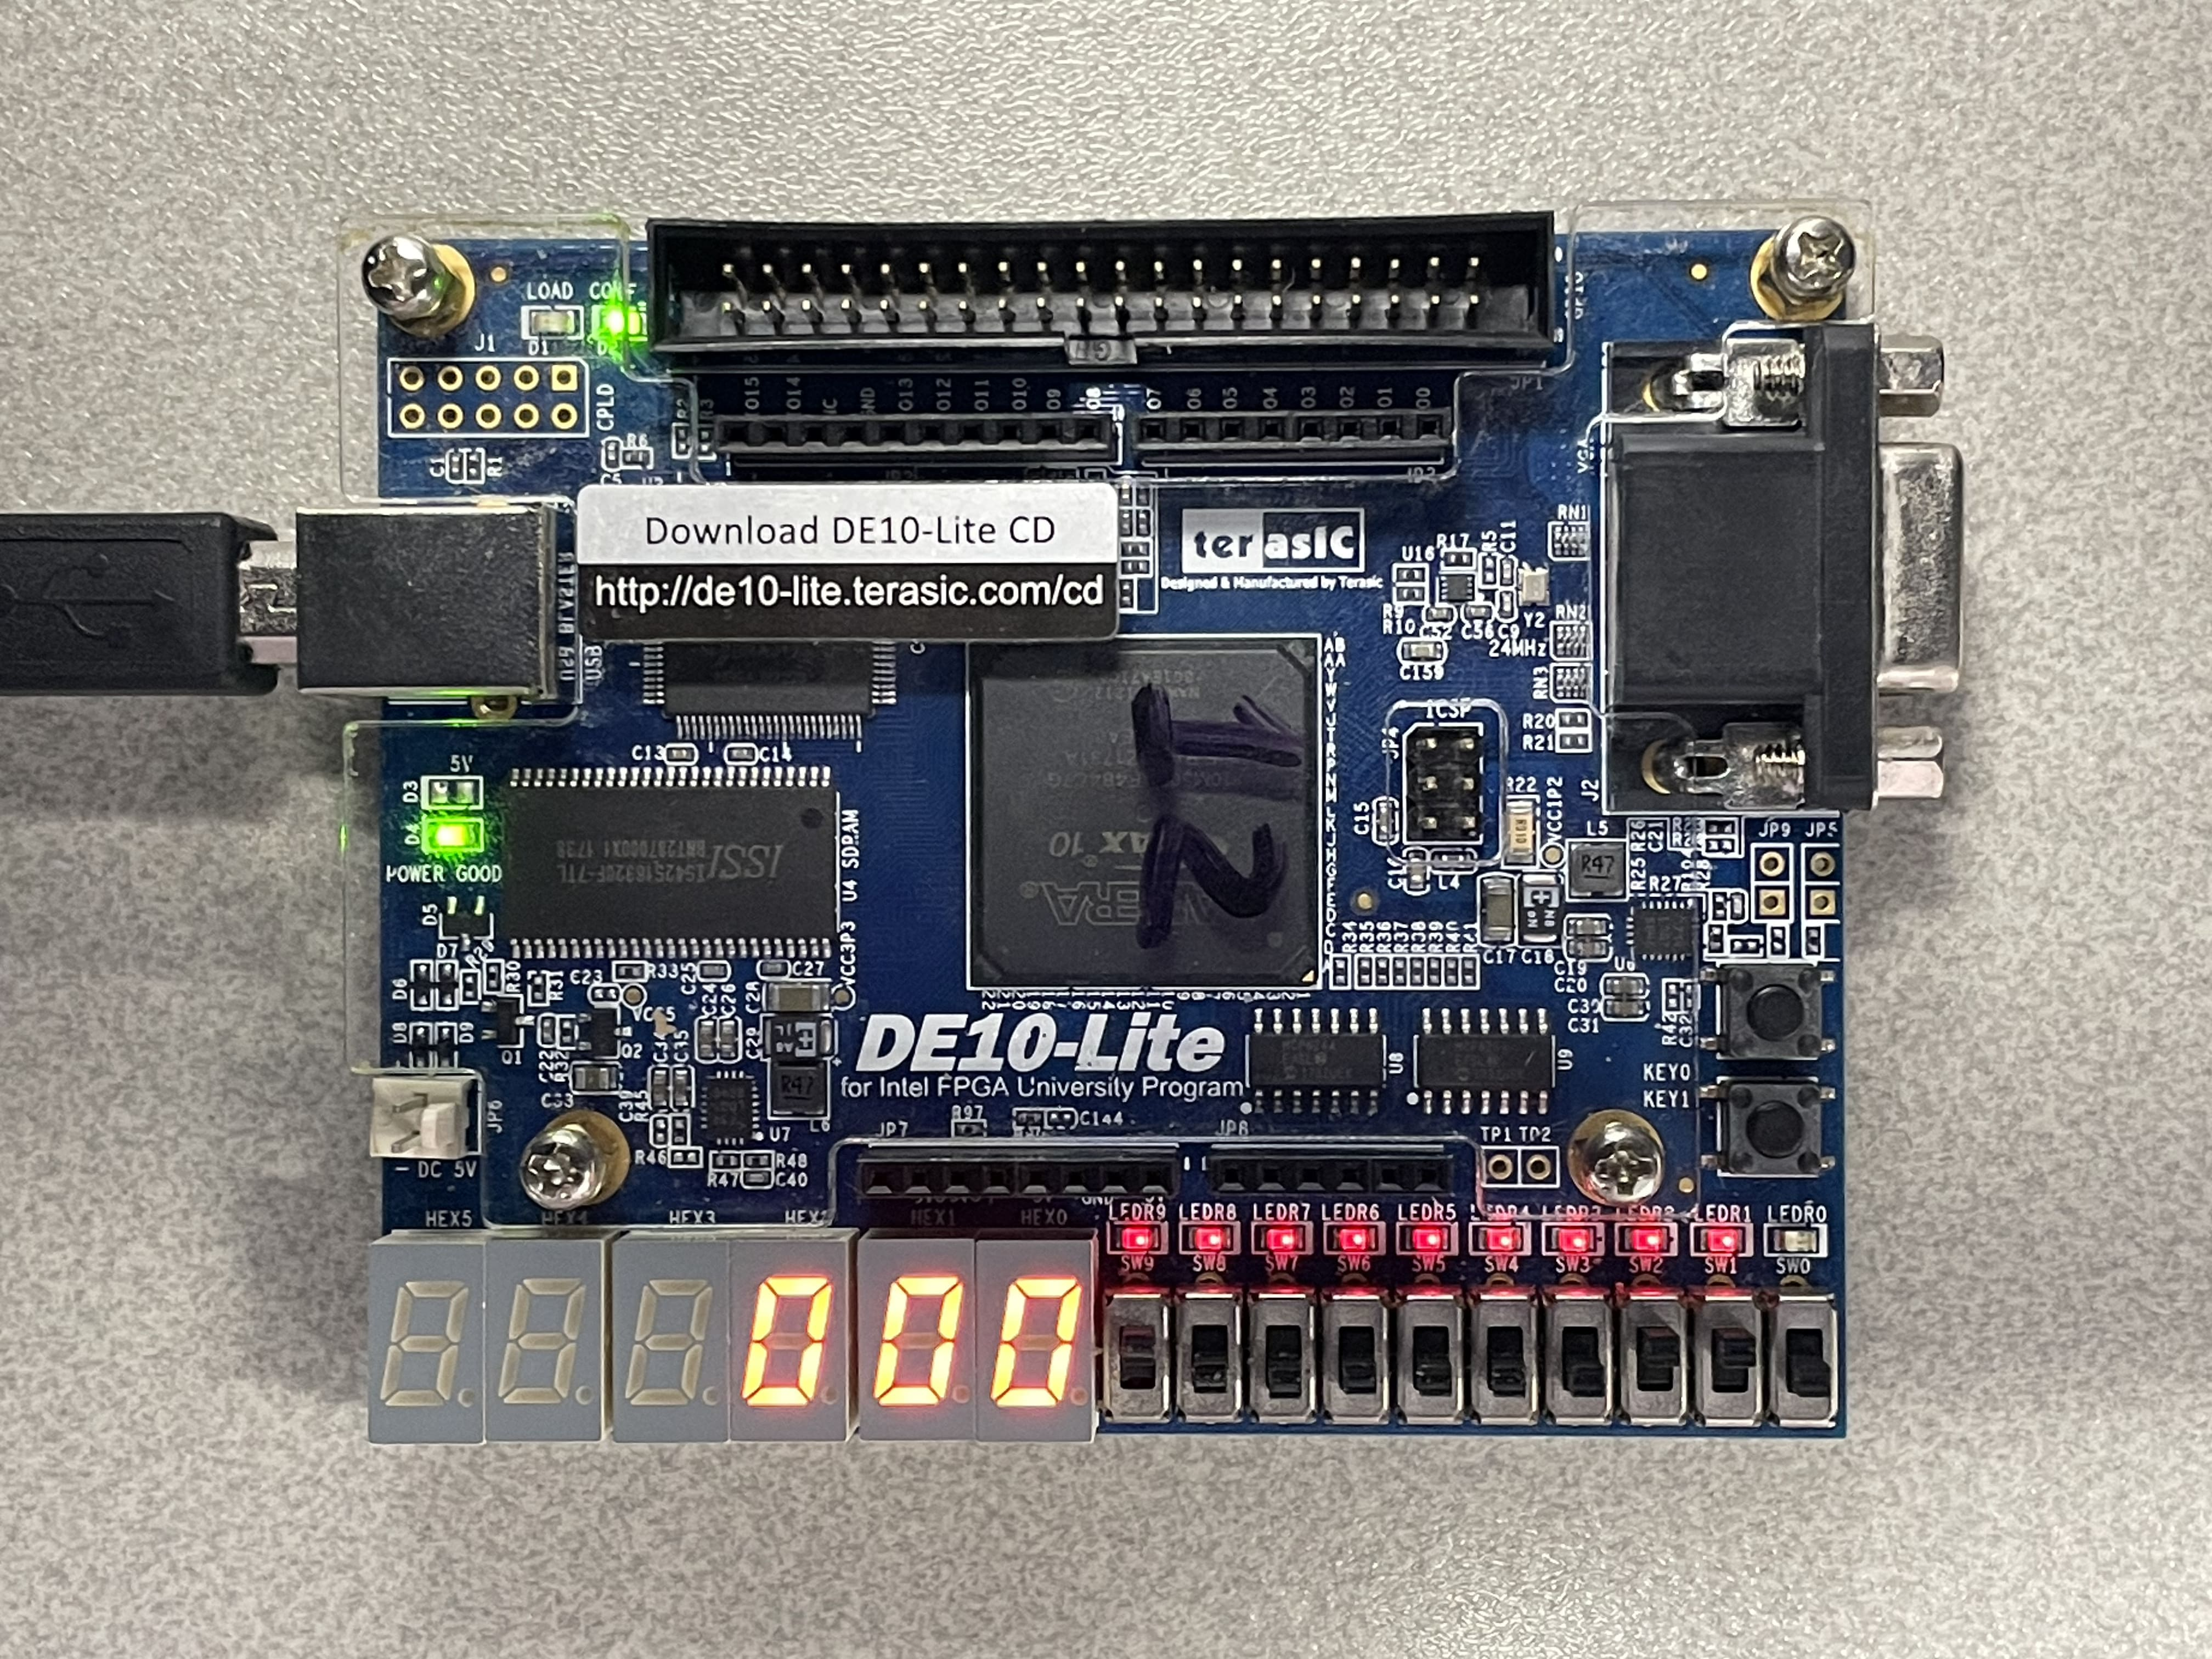
\includegraphics[width=.85\linewidth]{Montagem Laboratorial/images/IMG_2303.png}
        \caption{Teste na DE10-Lite (3)}\label{fig:DE3}
    \end{figure}
    \begin{figure}[H]
        \centering
        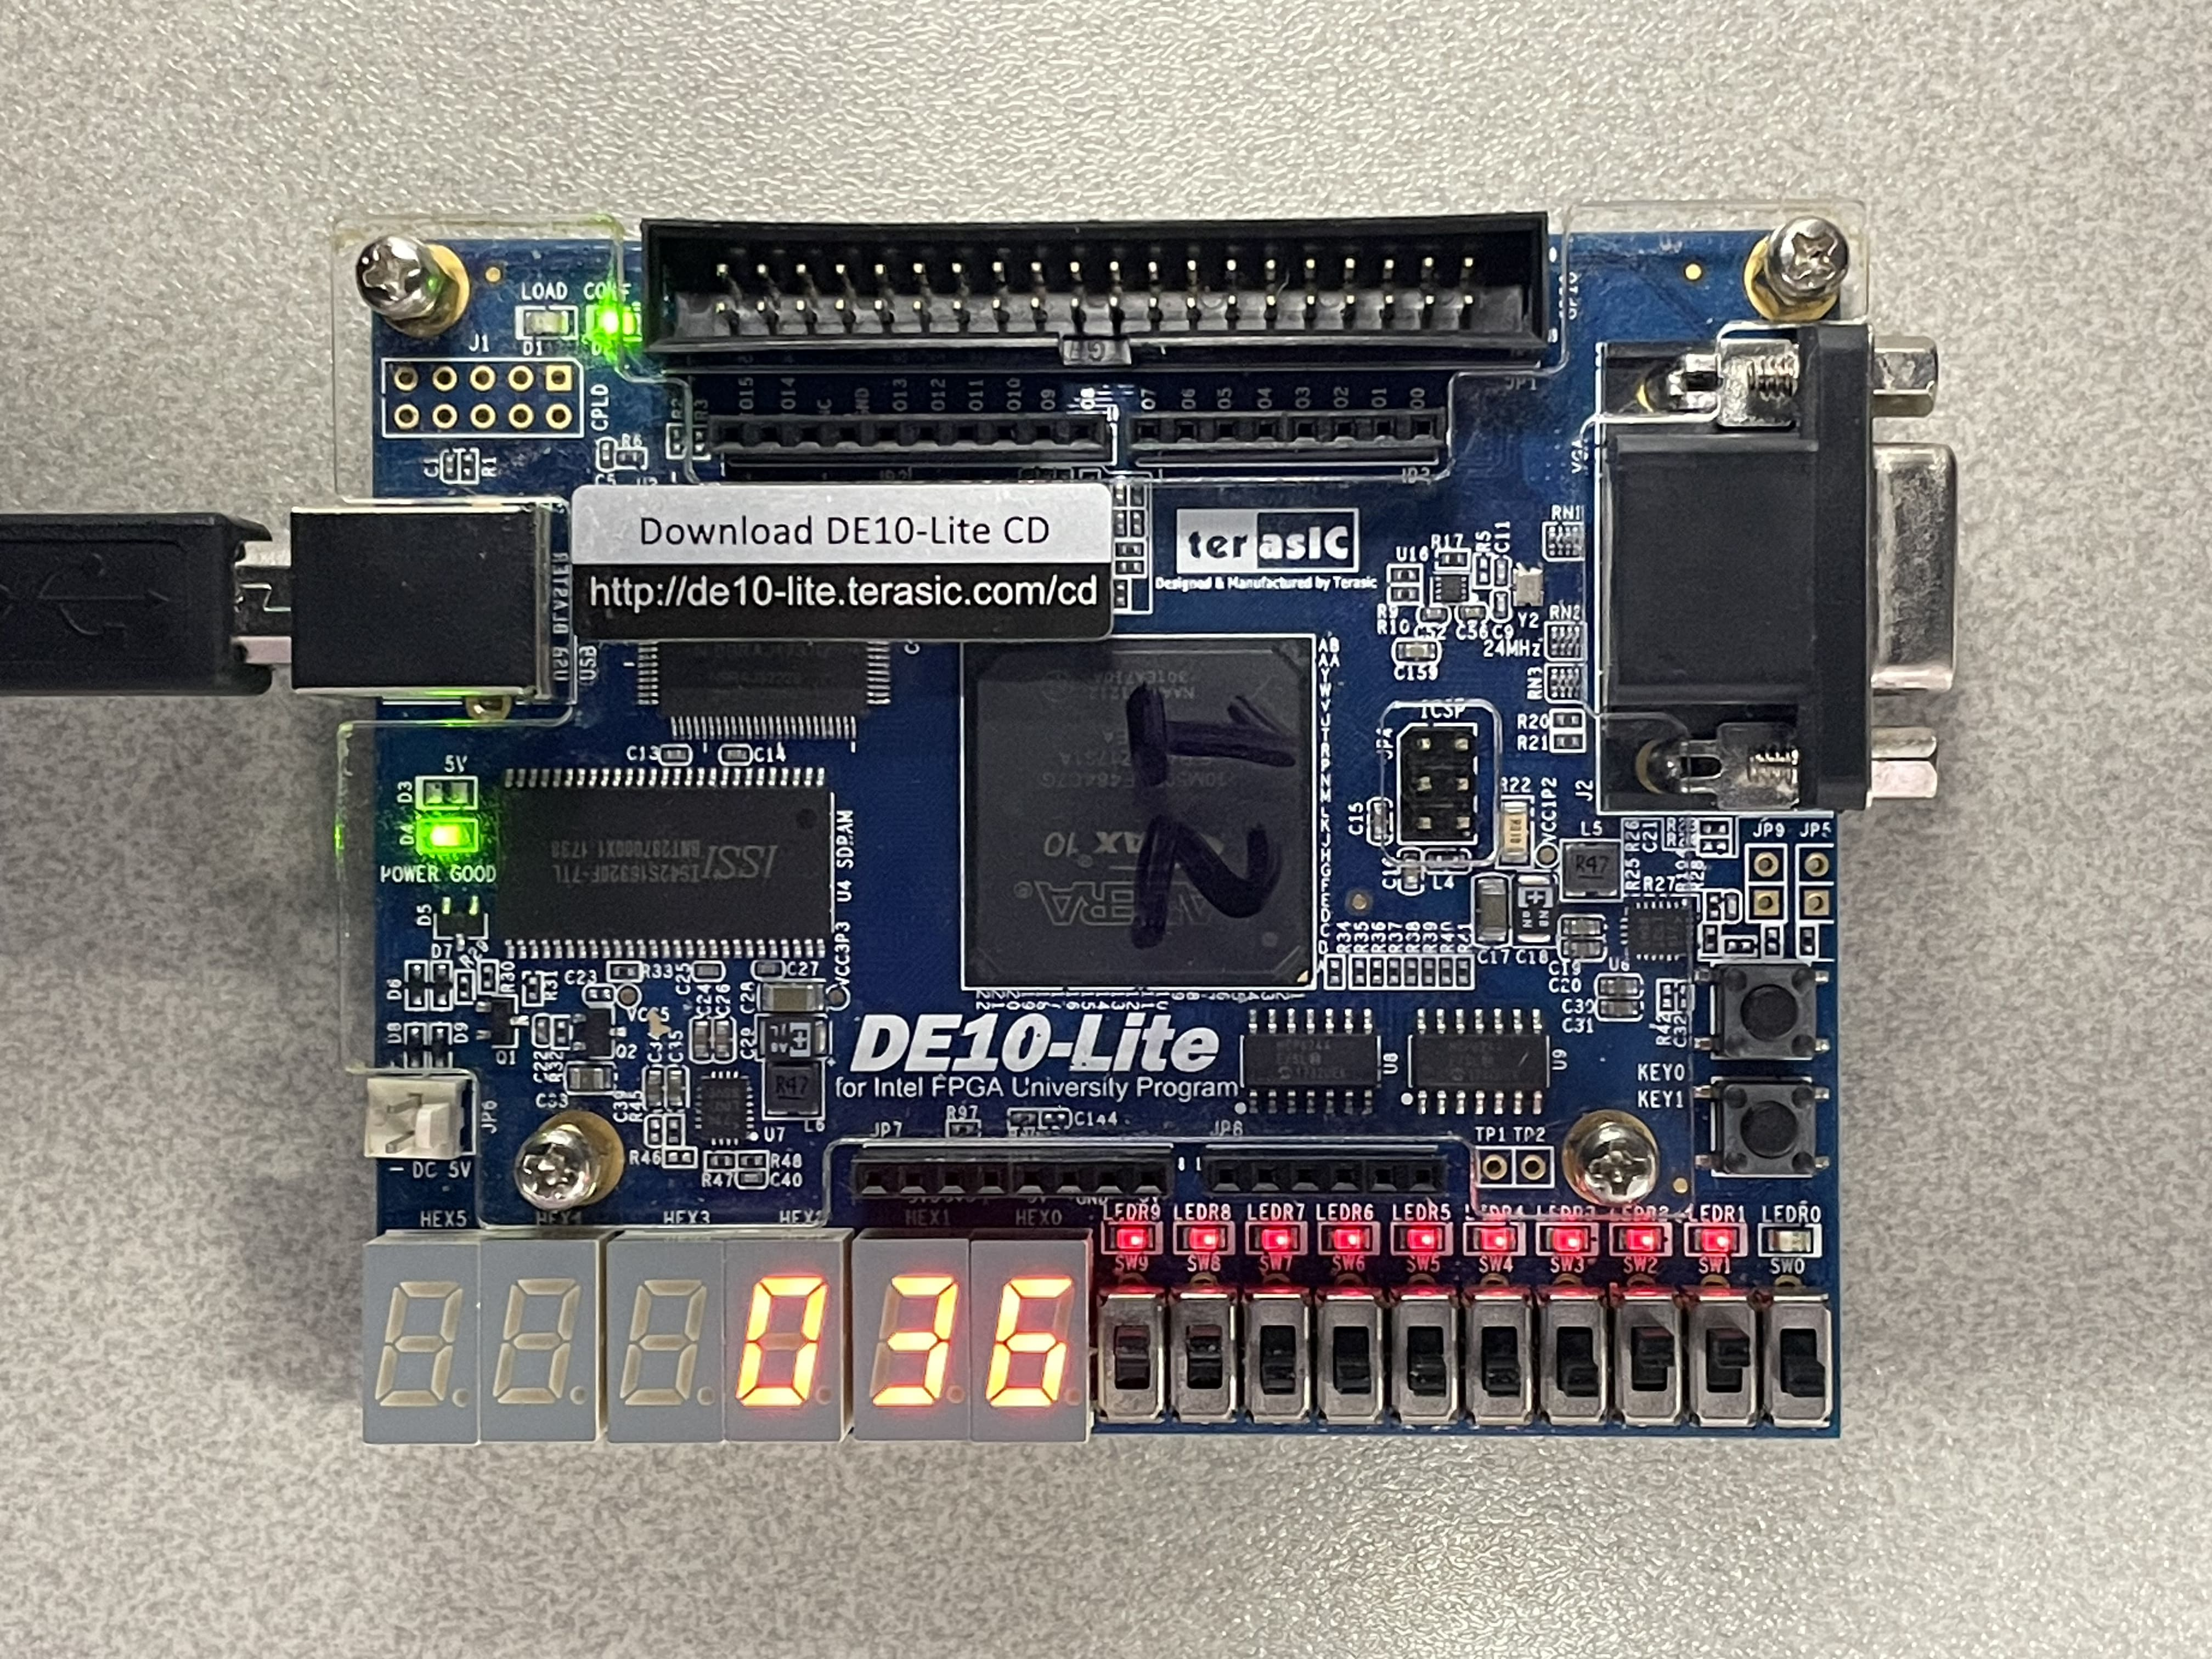
\includegraphics[width=.85\linewidth]{Montagem Laboratorial/images/IMG_2304.png}
        \caption{Teste na DE10-Lite (4)}\label{fig:DE4}
    \end{figure}
\end{multicols}

Na figura~\ref{fig:DE3}, introduzimos o valor que queremos adicionar, neste caso o 6. Ao acionar o Step, na figura~\ref{fig:DE4}, o sistema realiza o cálculo do quadrado da entrada, devolvendo 36 $(6^2)$.
\vspace*{\fill}%
\newpage
\vspace*{\fill}
\begin{multicols}{2}
    \begin{figure}[H]
        \centering
        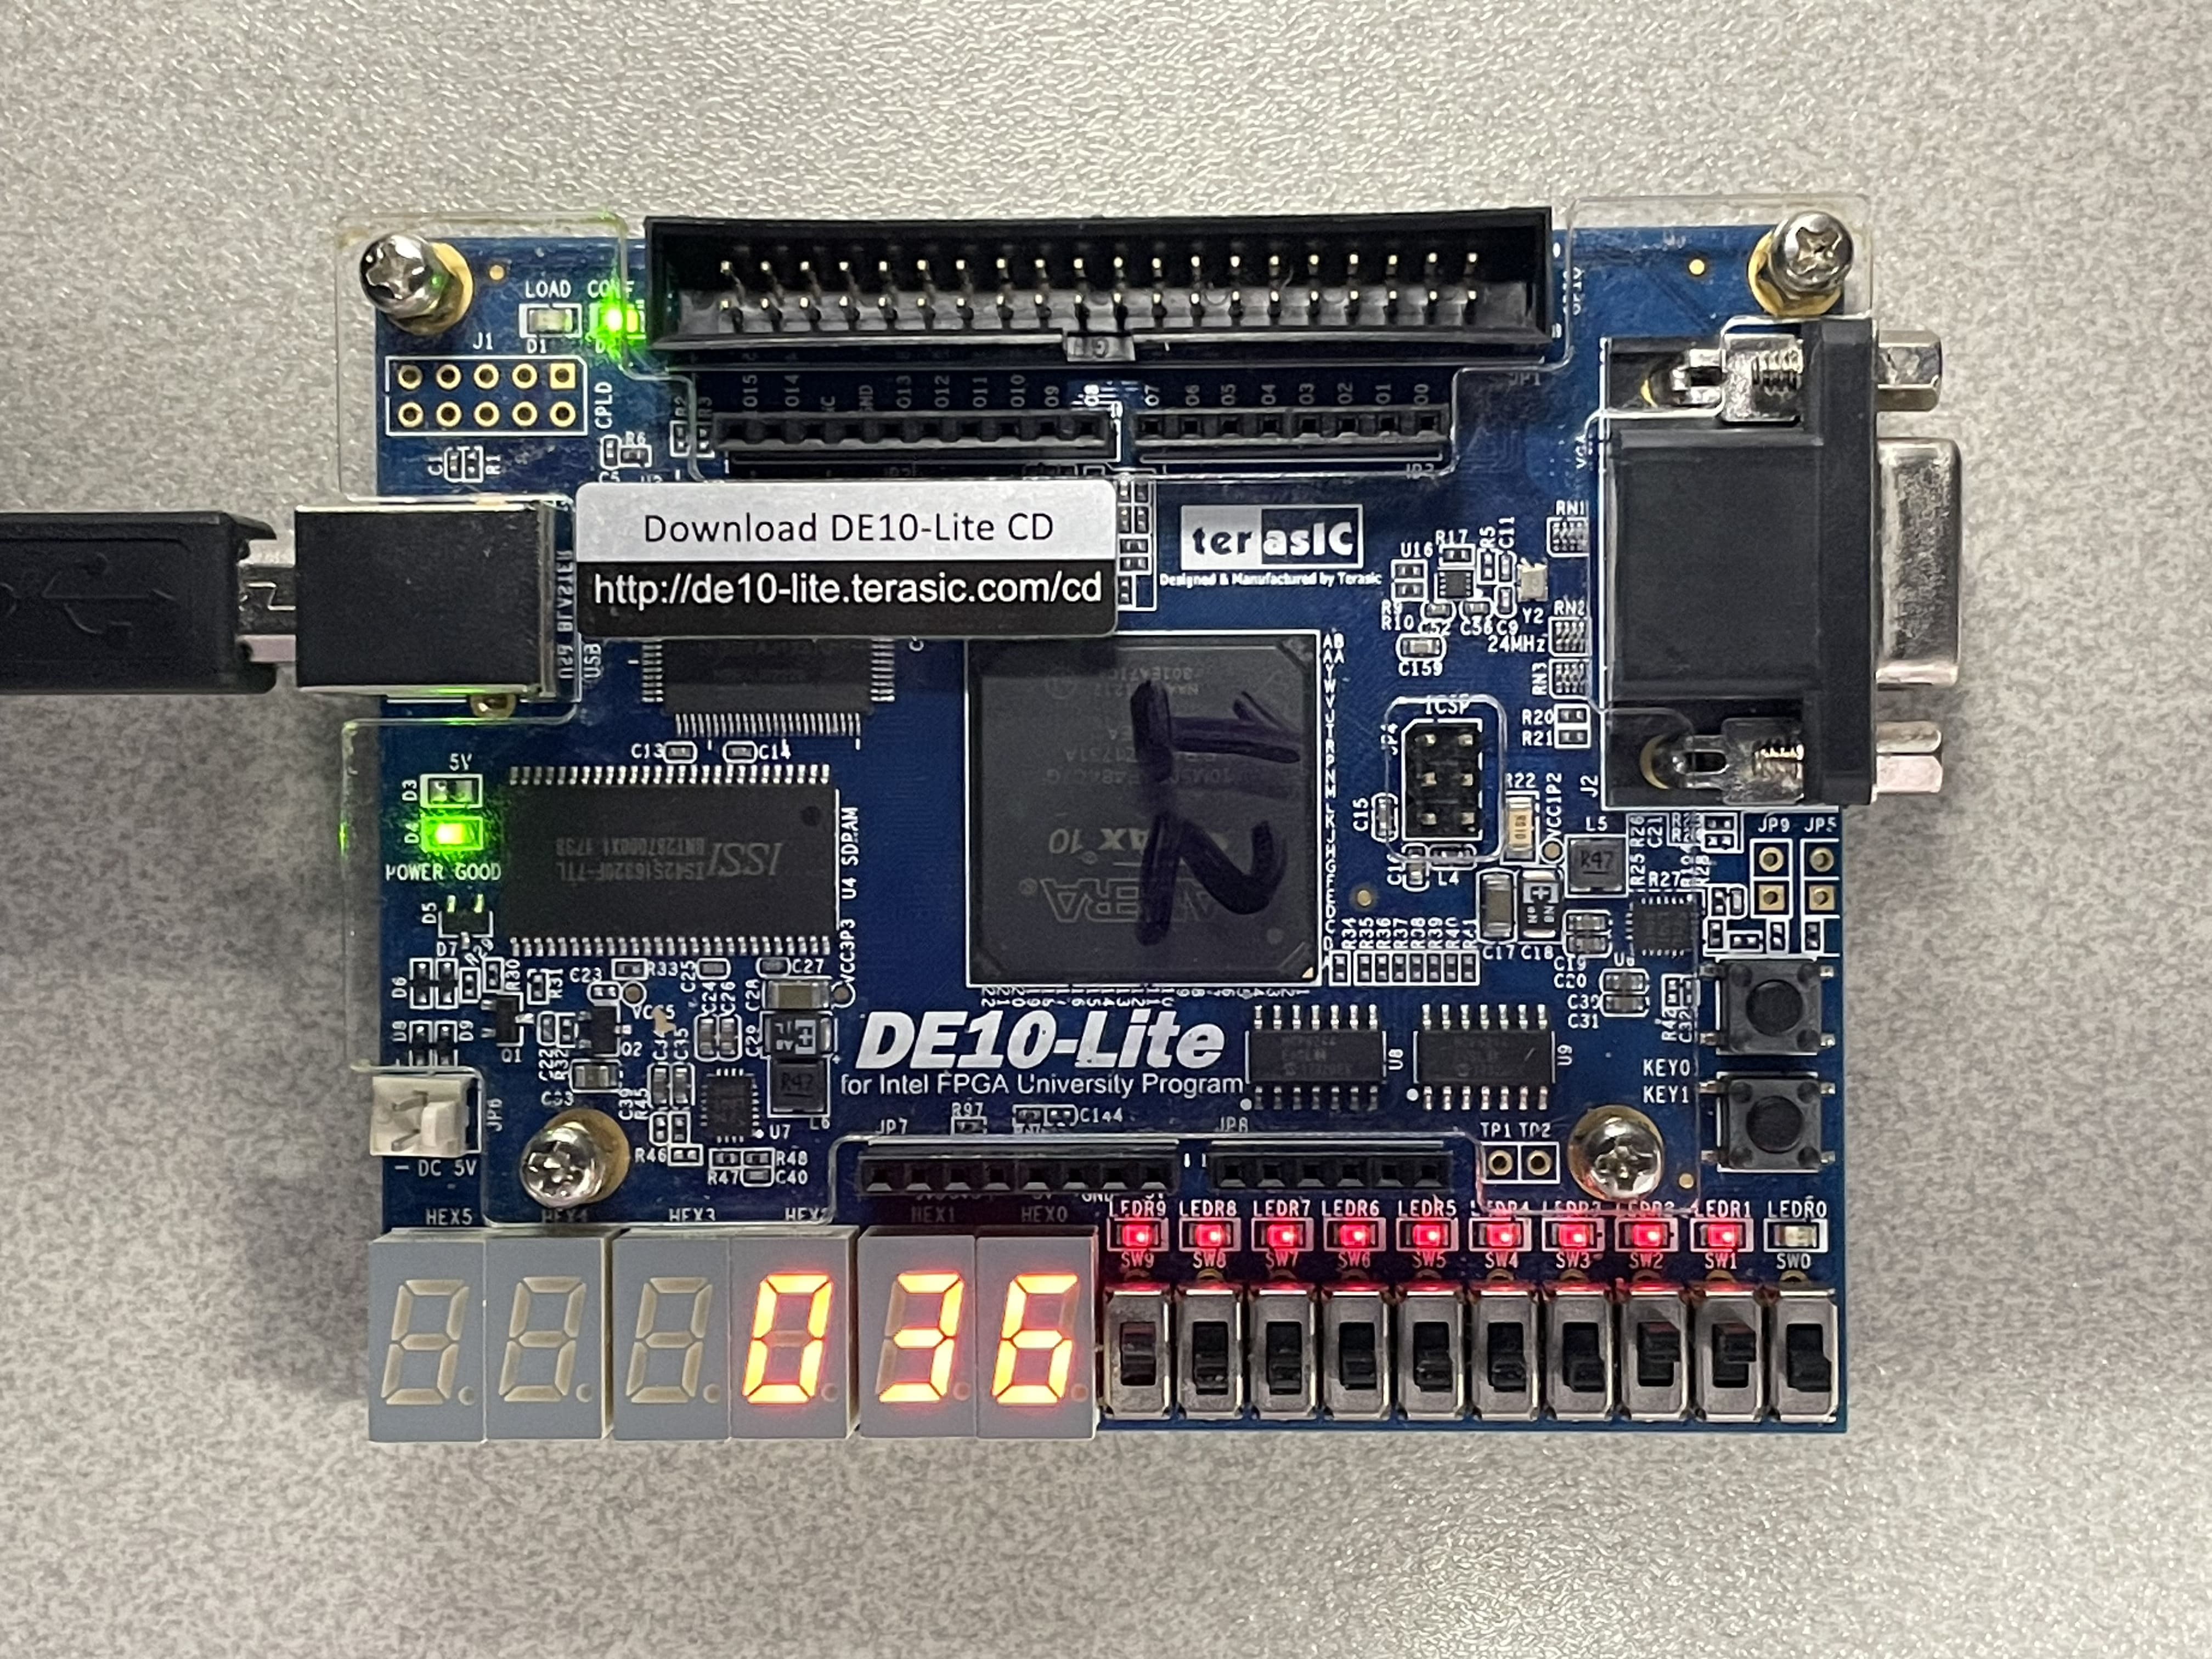
\includegraphics[width=.85\linewidth]{Montagem Laboratorial/images/IMG_2305.png}
        \caption{Teste na DE10-Lite (5)}\label{fig:DE5}
    \end{figure}
    \begin{figure}[H]
        \centering
        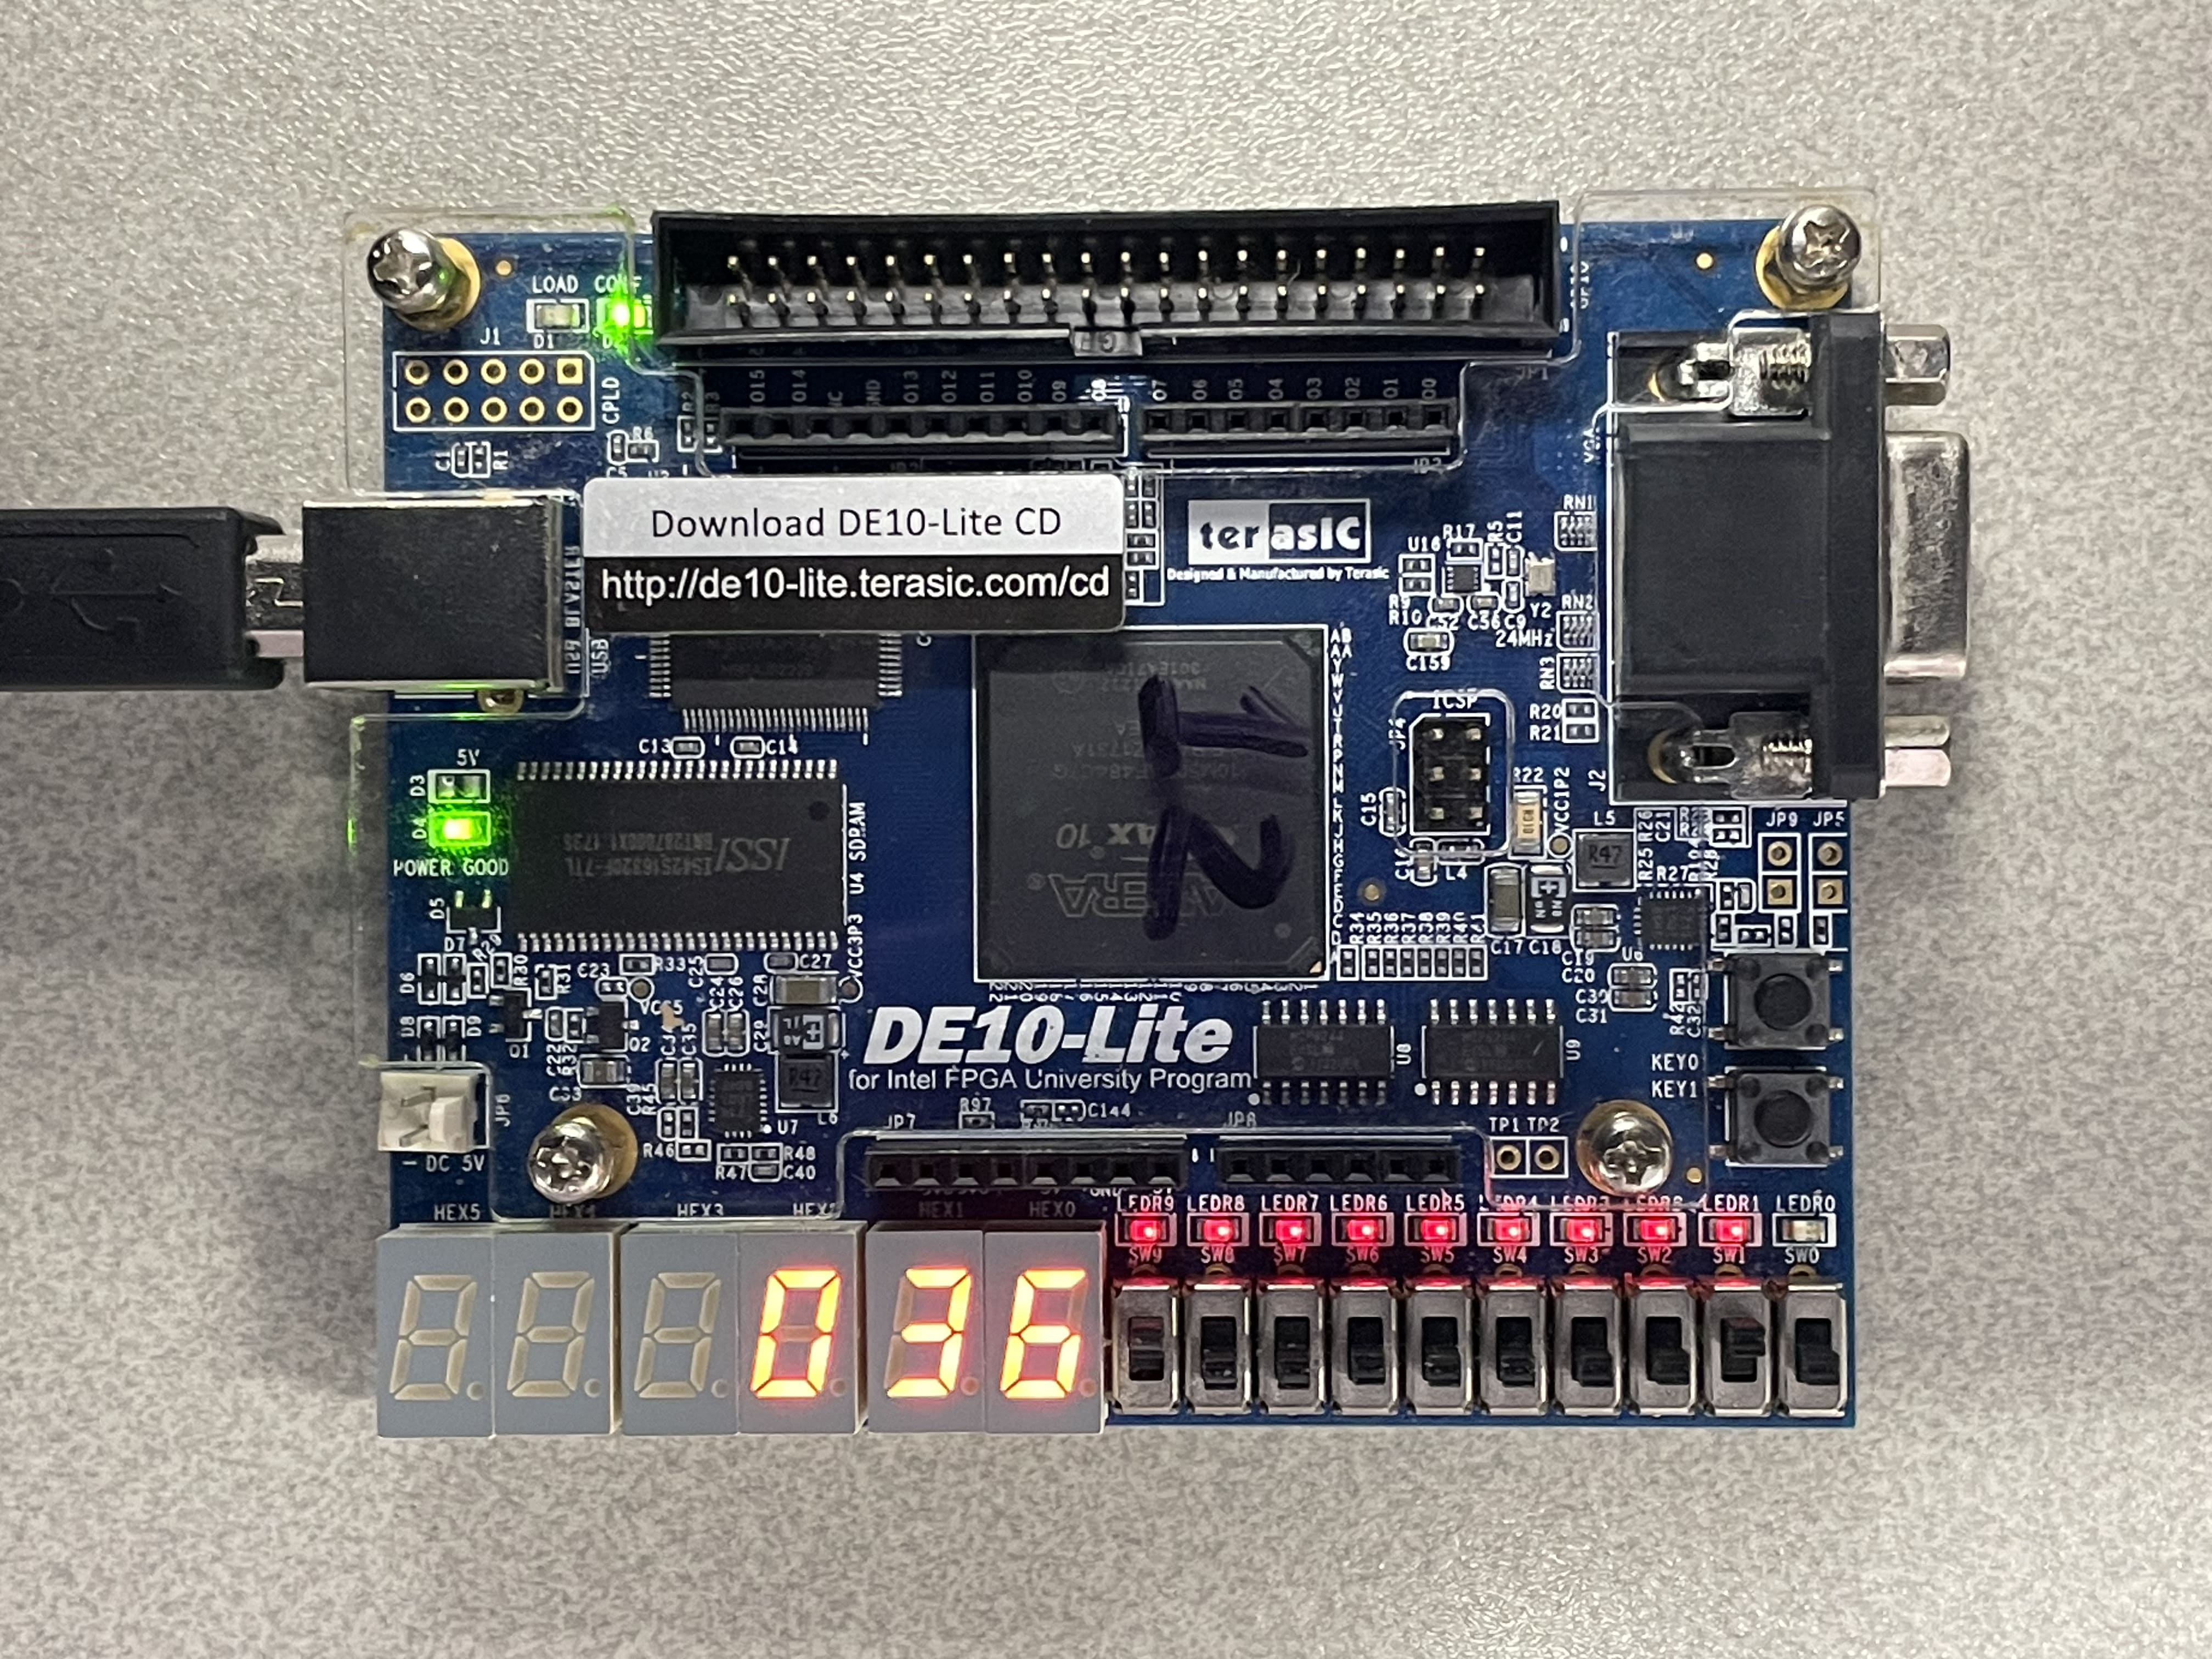
\includegraphics[width=.85\linewidth]{Montagem Laboratorial/images/IMG_2306.png}
        \caption{Teste na DE10-Lite (6)}\label{fig:DE6}
    \end{figure}
\end{multicols}

De seguida, na figura~\ref{fig:DE5}, desativamos o Step. Ainda estamos a visualizar o valor do quadrado, mas neste caso, já é o valor acumulado. Na figura~\ref{fig:DE6}, introduzimos um novo valor de $x$, neste caso o 2.

\begin{multicols}{2}
    \begin{figure}[H]
        \centering
        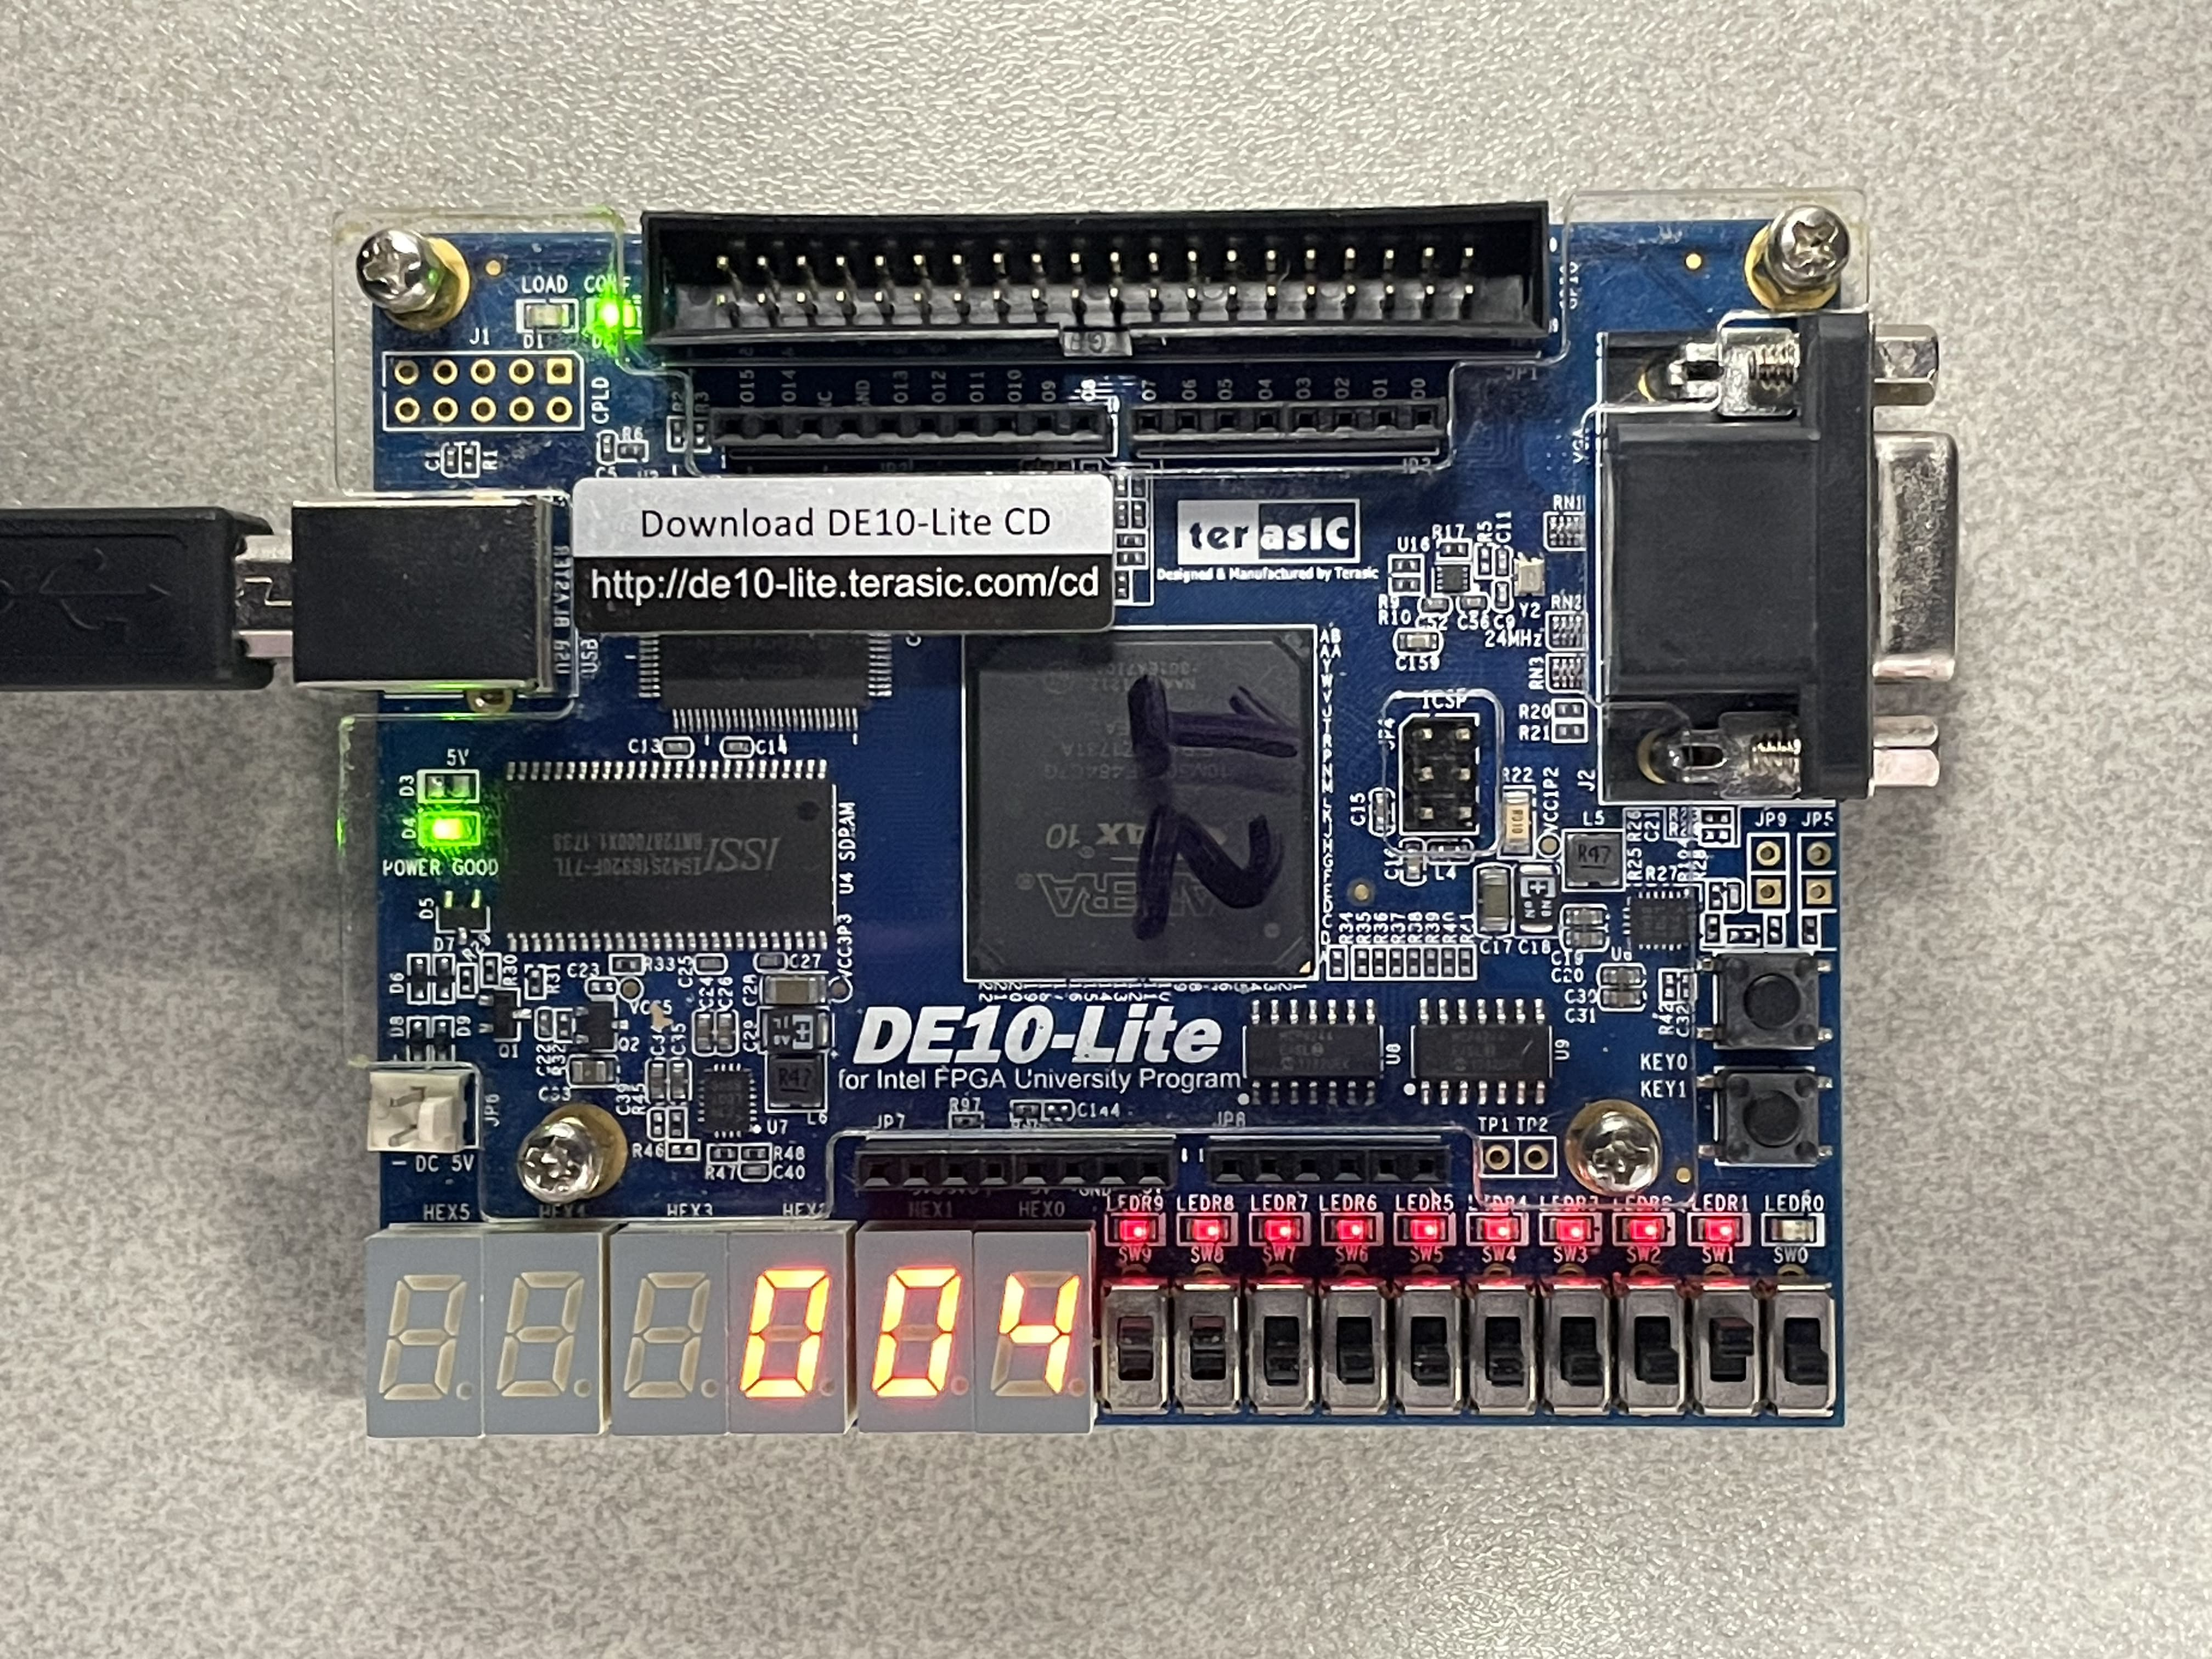
\includegraphics[width=.85\linewidth]{Montagem Laboratorial/images/IMG_2308.png}
        \caption{Teste na DE10-Lite (7)}\label{fig:DE7}
    \end{figure}
    \begin{figure}[H]
        \centering
        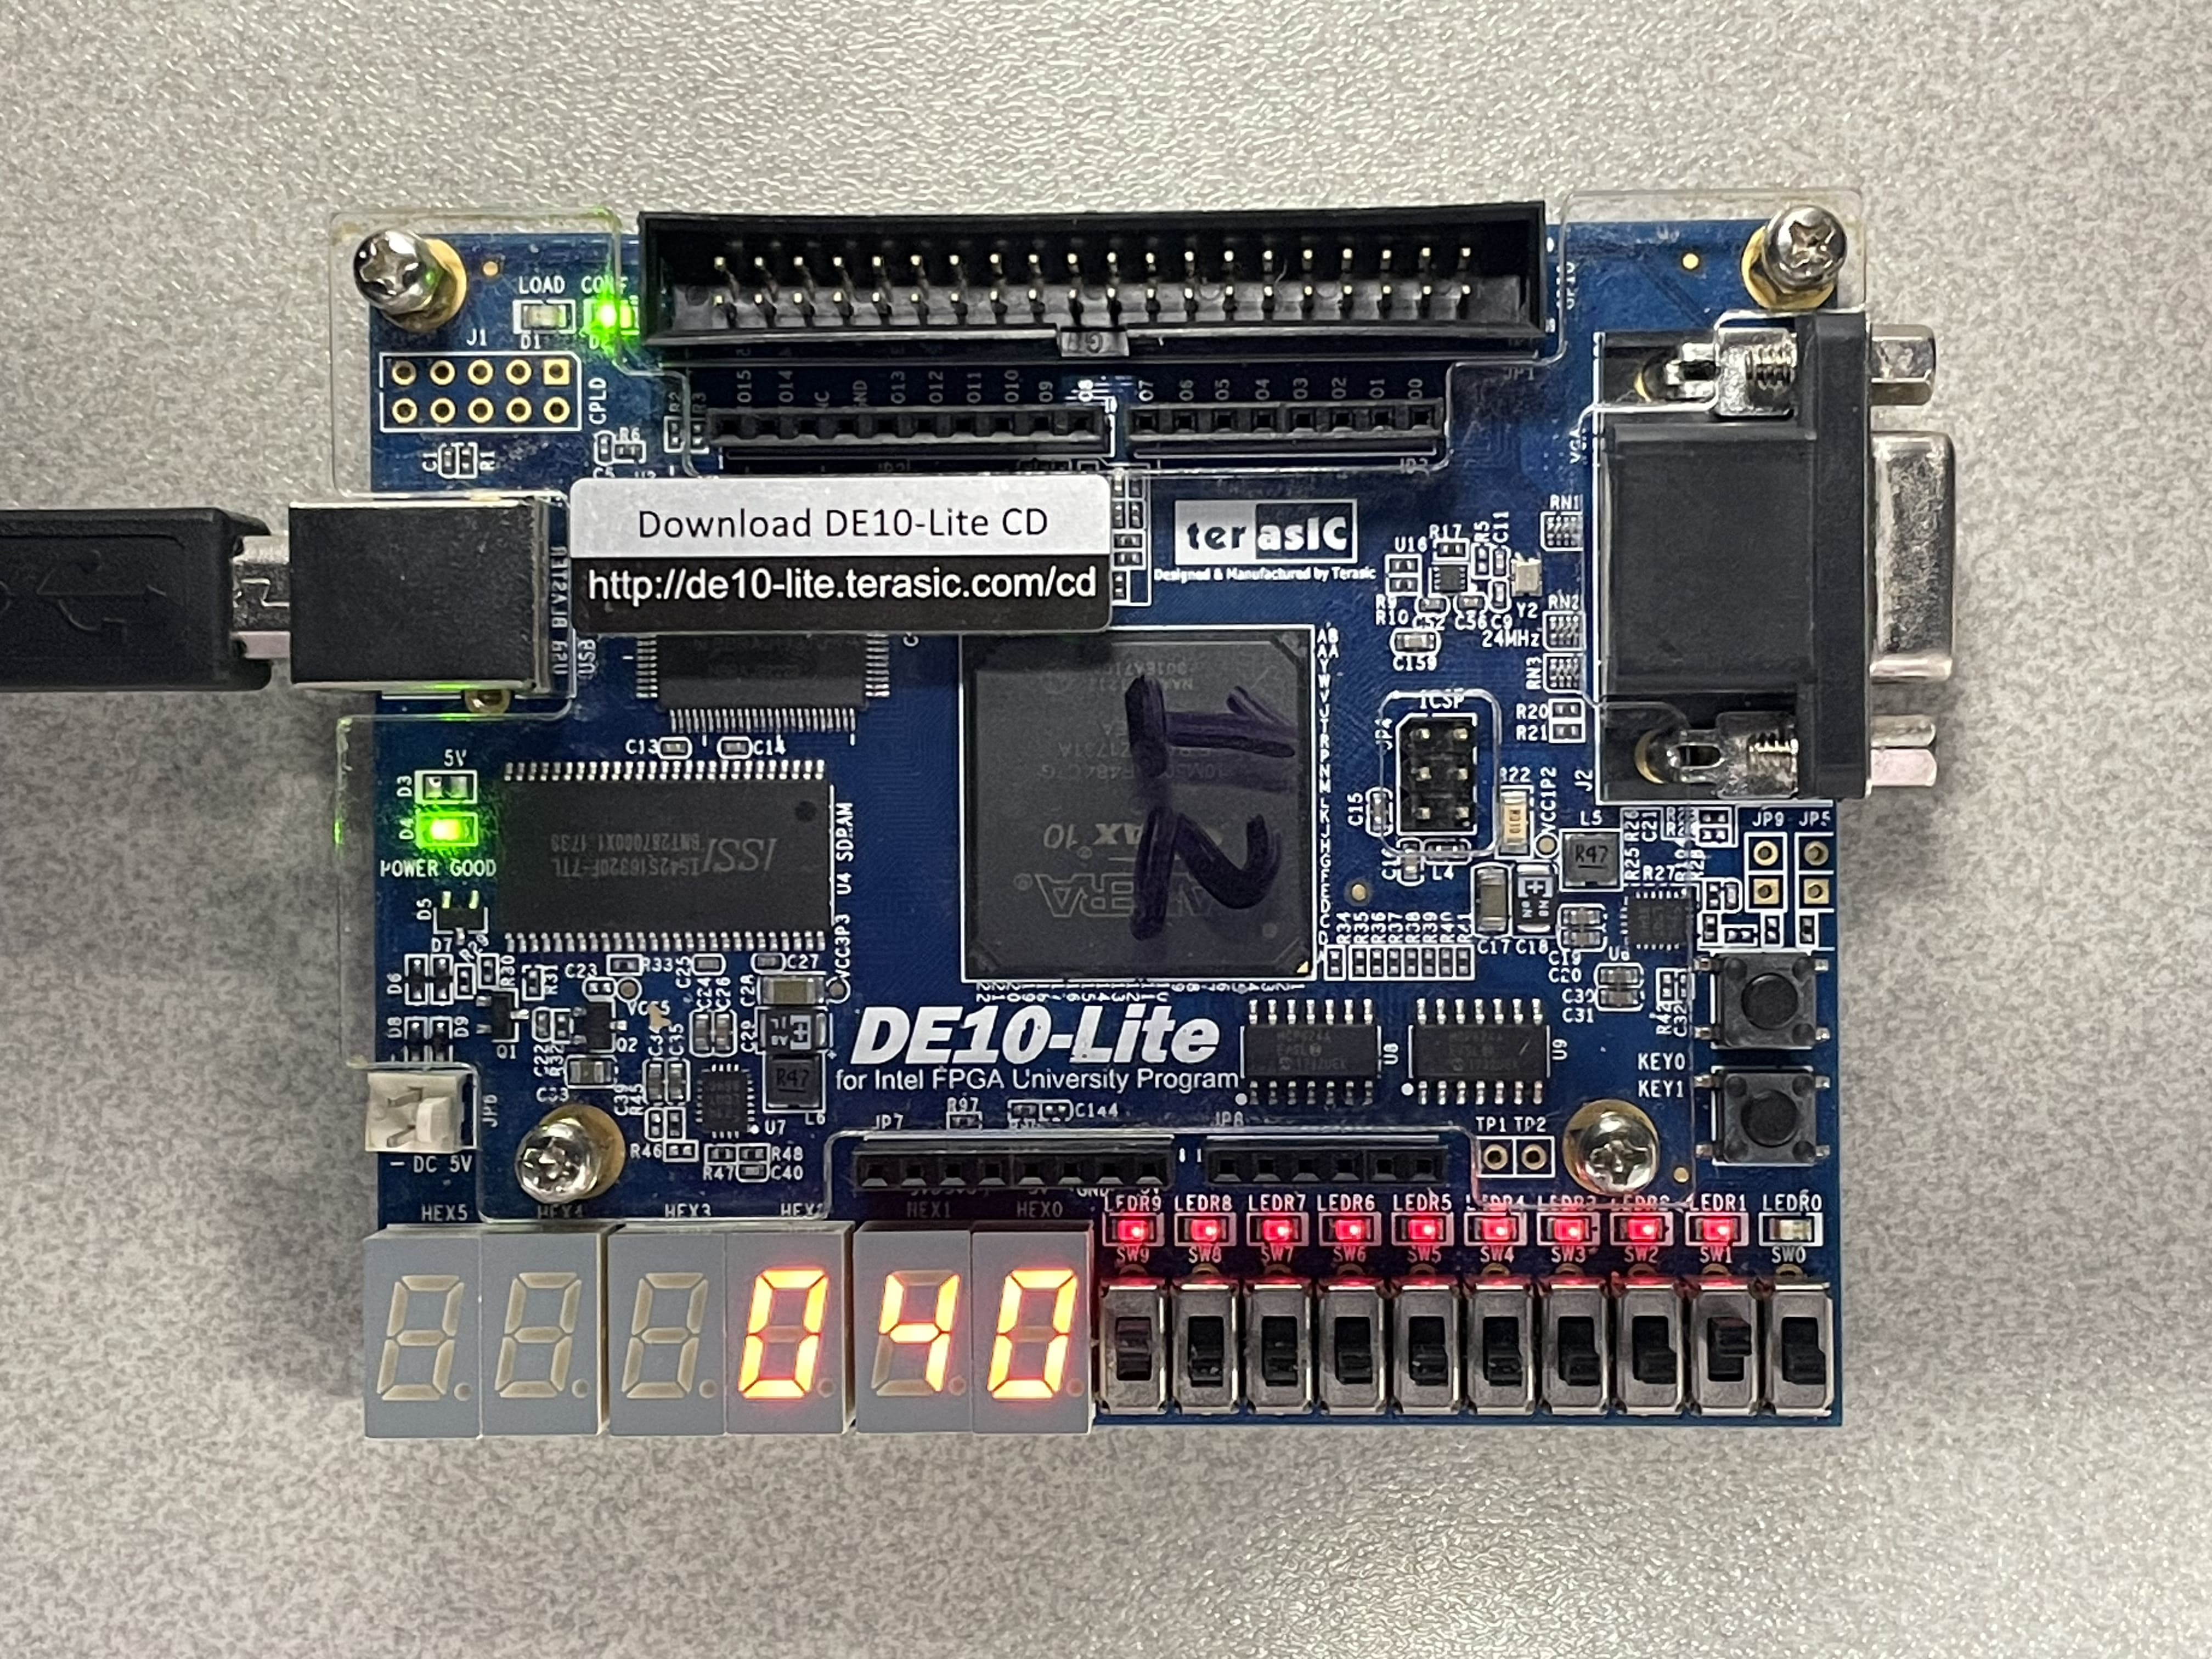
\includegraphics[width=.85\linewidth]{Montagem Laboratorial/images/IMG_2309.png}
        \caption{Teste na DE10-Lite (8)}\label{fig:DE8}
    \end{figure}
\end{multicols}

Ao acionar o Step, na figura~\ref{fig:DE7}, o sistema realiza o cálculo do quadrado da entrada e devolve 4 $(2^2)$. Ao desativar o Step, na figura~\ref{fig:DE8}, o sistema devolve o novo valor acumulado.

\vspace*{\fill}%

\newpage

\vspace*{\fill}

\begin{multicols}{2}
    \begin{figure}[H]
        \centering
        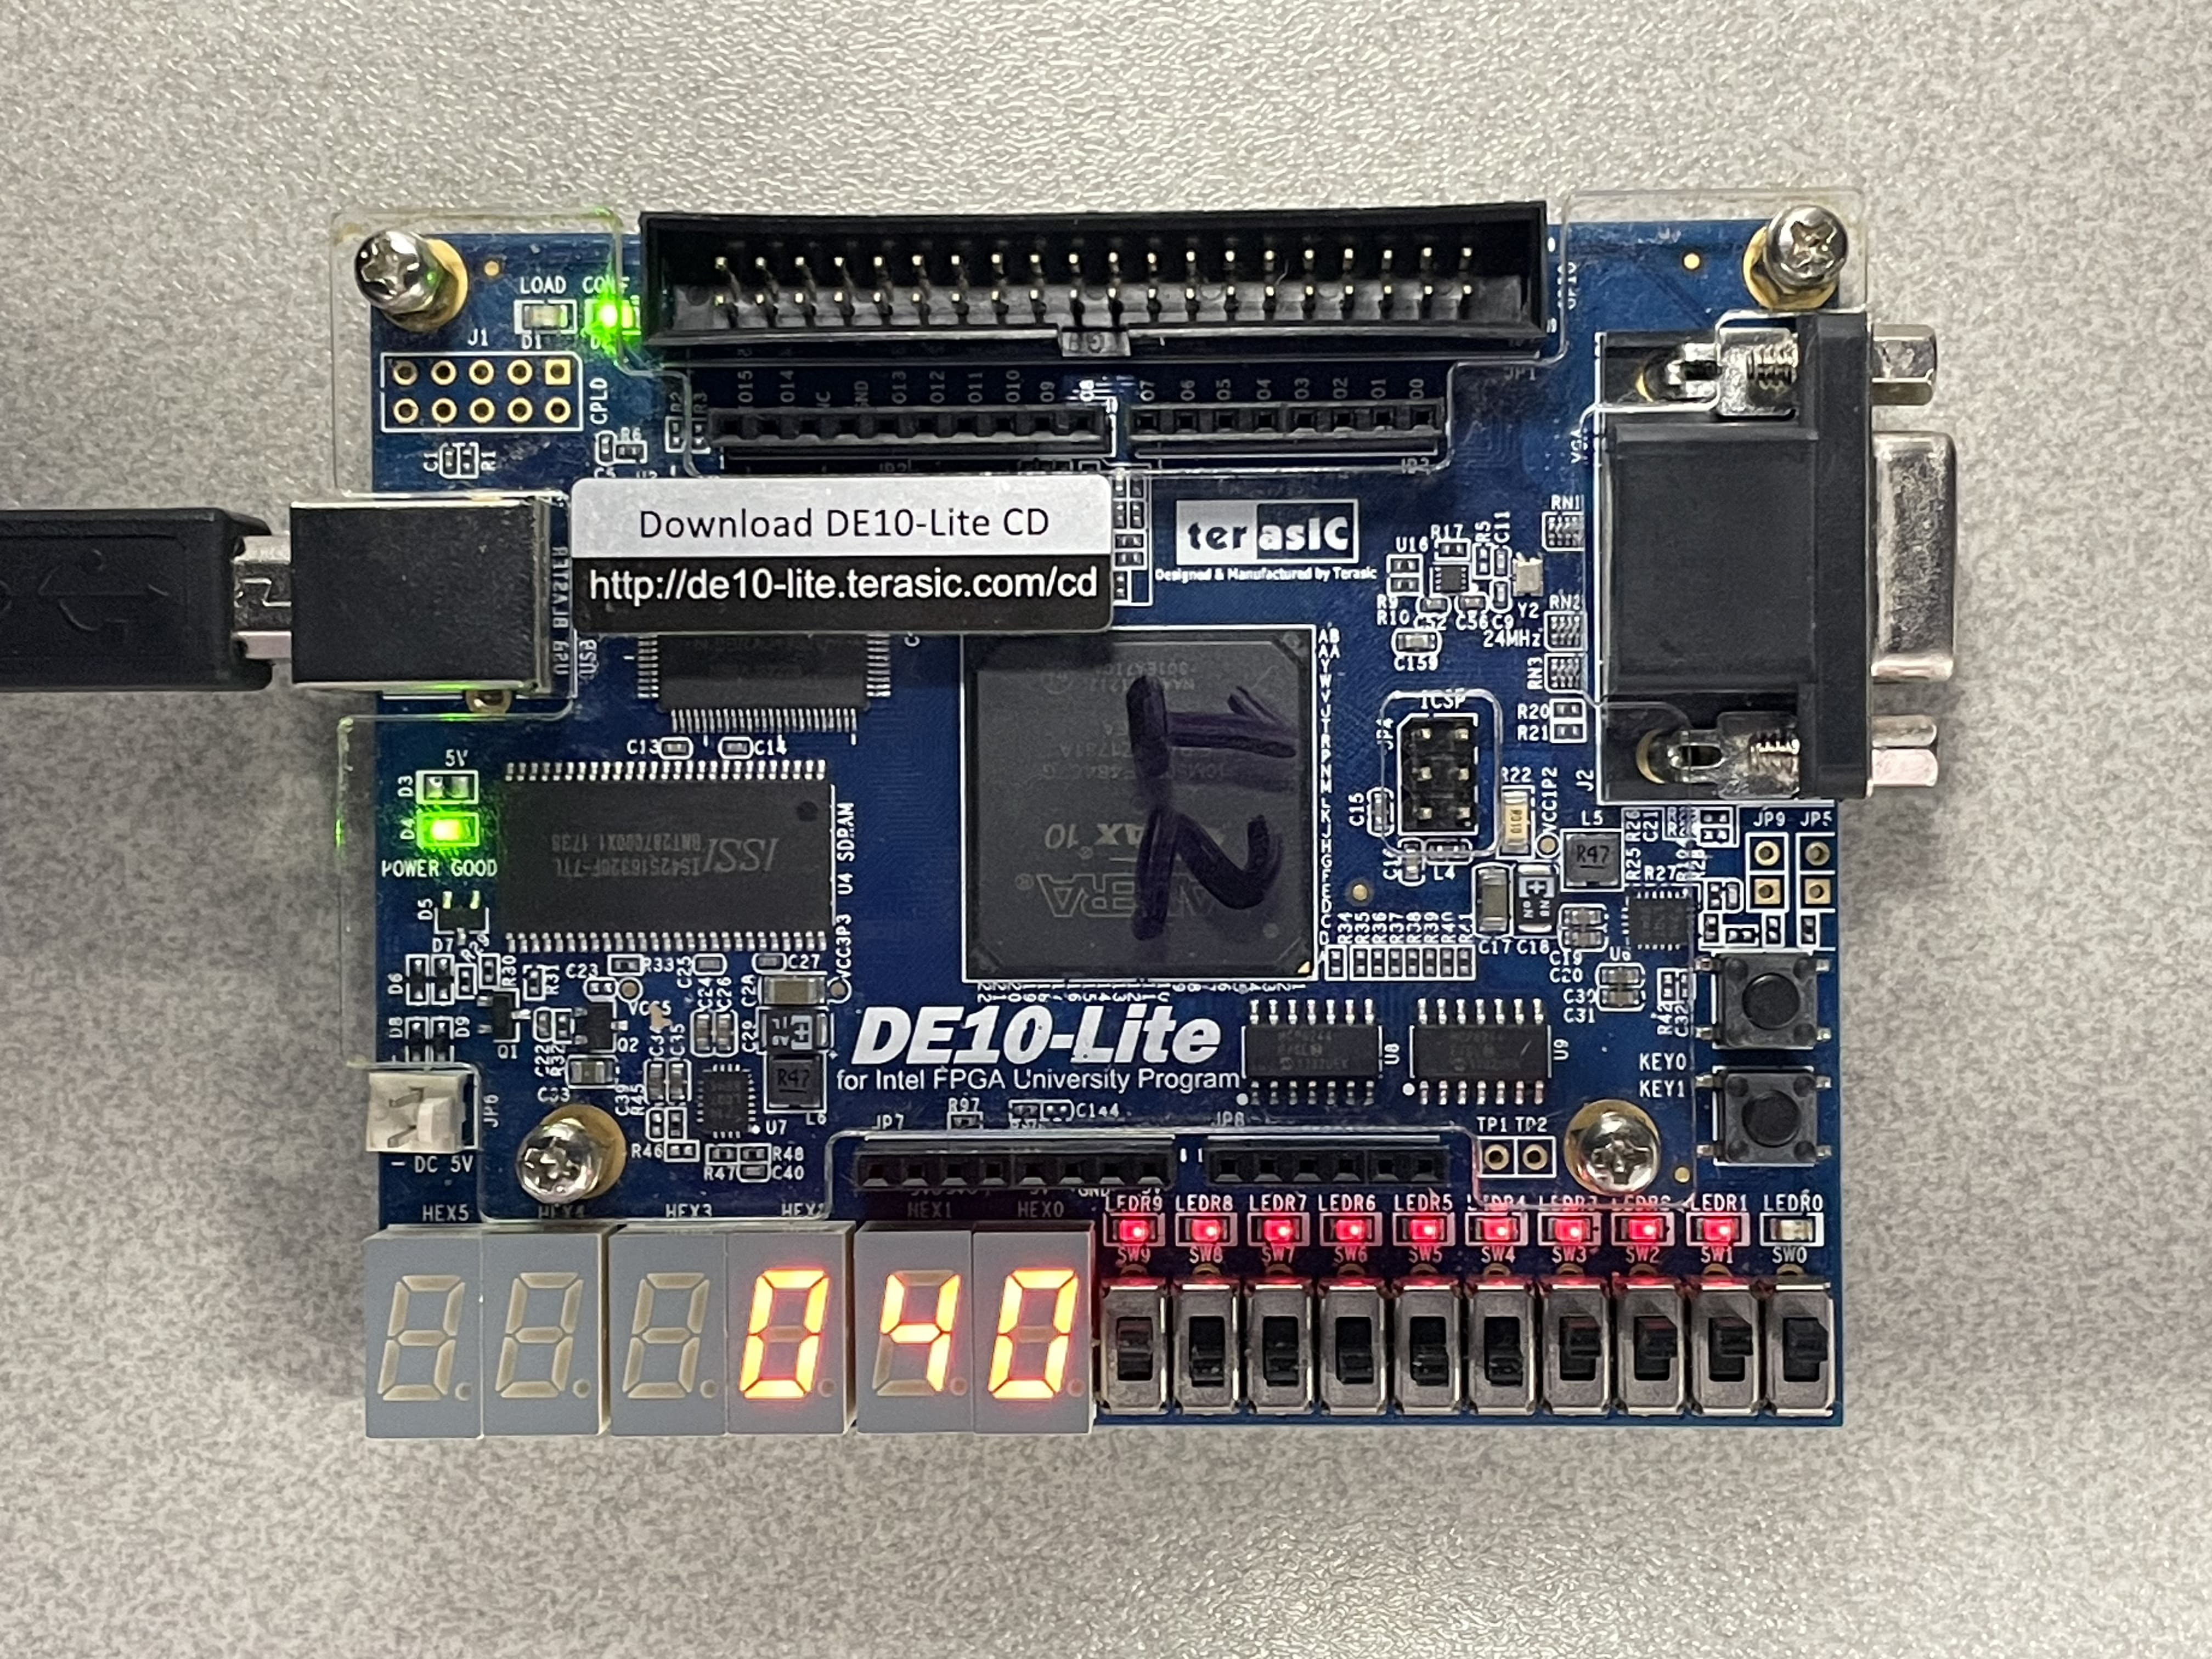
\includegraphics[width=.85\linewidth]{Montagem Laboratorial/images/IMG_2310.png}
        \caption{Teste na DE10-Lite (9)}\label{fig:DE9}
    \end{figure}
    \begin{figure}[H]
        \centering
        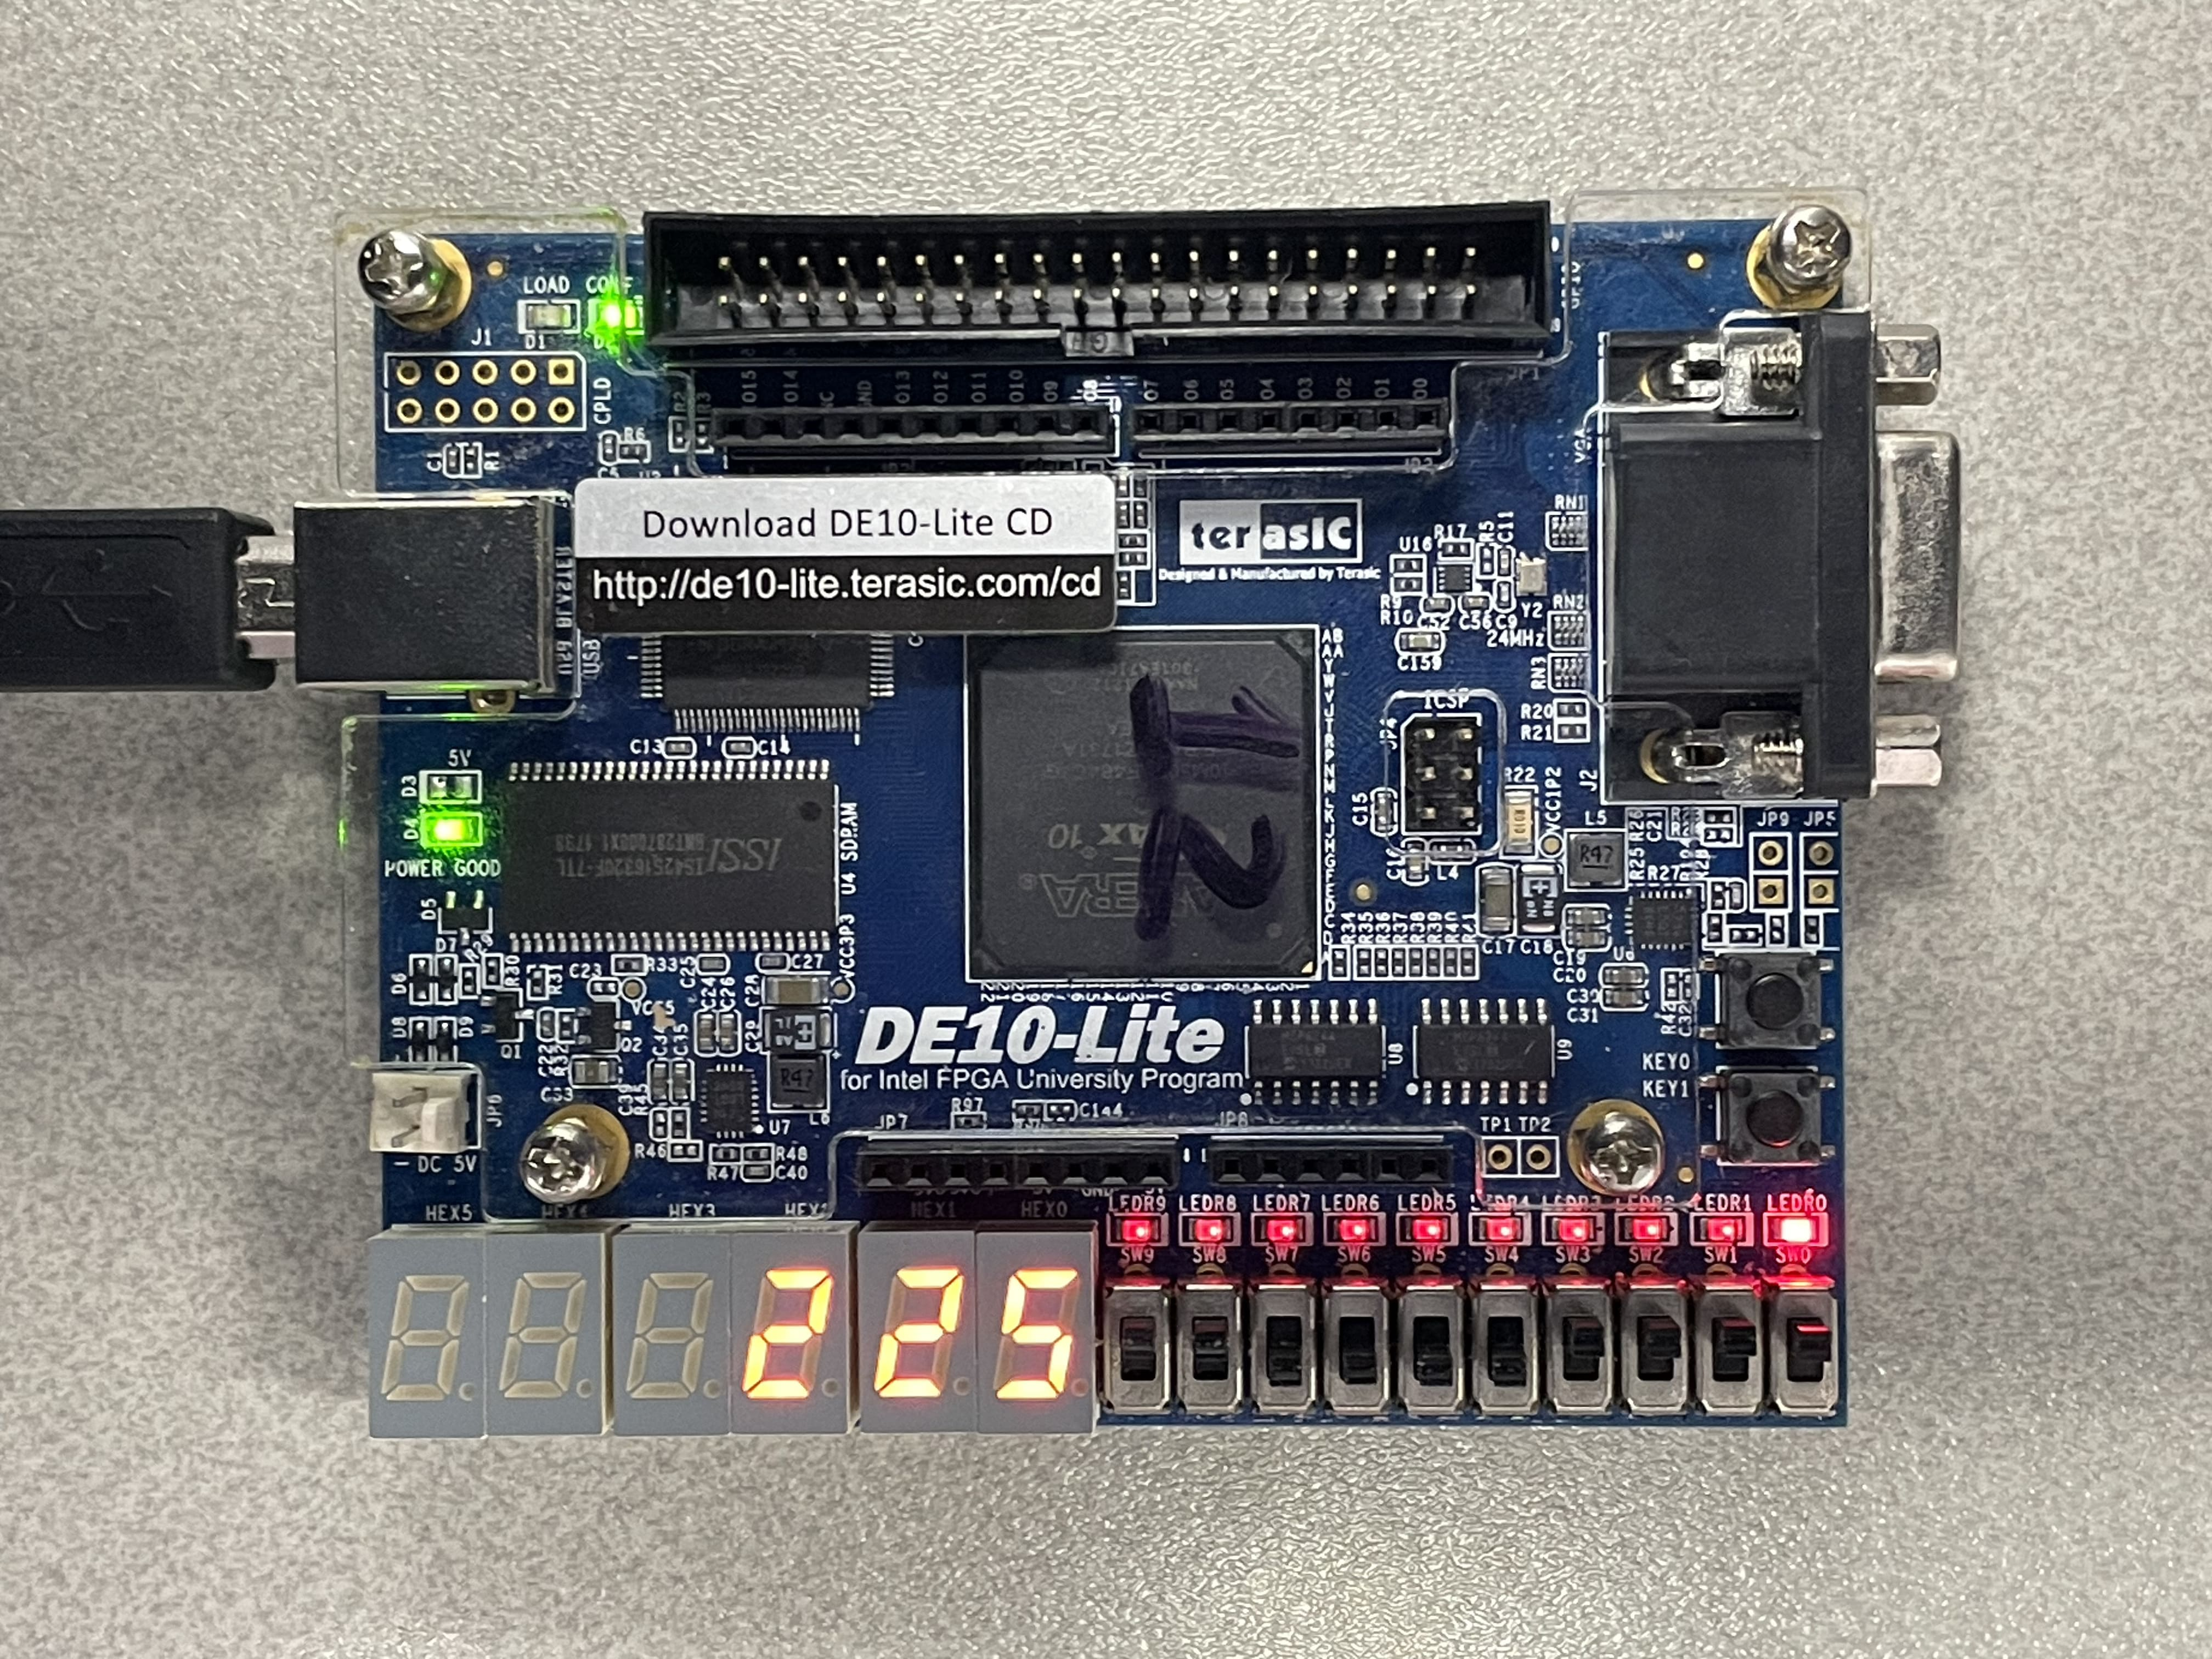
\includegraphics[width=.85\linewidth]{Montagem Laboratorial/images/IMG_2311.png}
        \caption{Teste na DE10-Lite (10)}\label{fig:DE10}
    \end{figure}
\end{multicols}

Na figura~\ref{fig:DE9}, introduzimos um novo valor para realizar o calculo, sendo ele o 15. Ao acionar o Step, na figura~\ref{fig:DE10}, o sistema realiza o cálculo do quadrado da entrada, devolvendo 225 $(15^2)$. Como a soma acumulada passou do limite de representação $(40 + 225 = 265 \not< 255)$, o \gls{led} do Cy acendeu. 

\begin{multicols}{2}
    \begin{figure}[H]
        \centering
        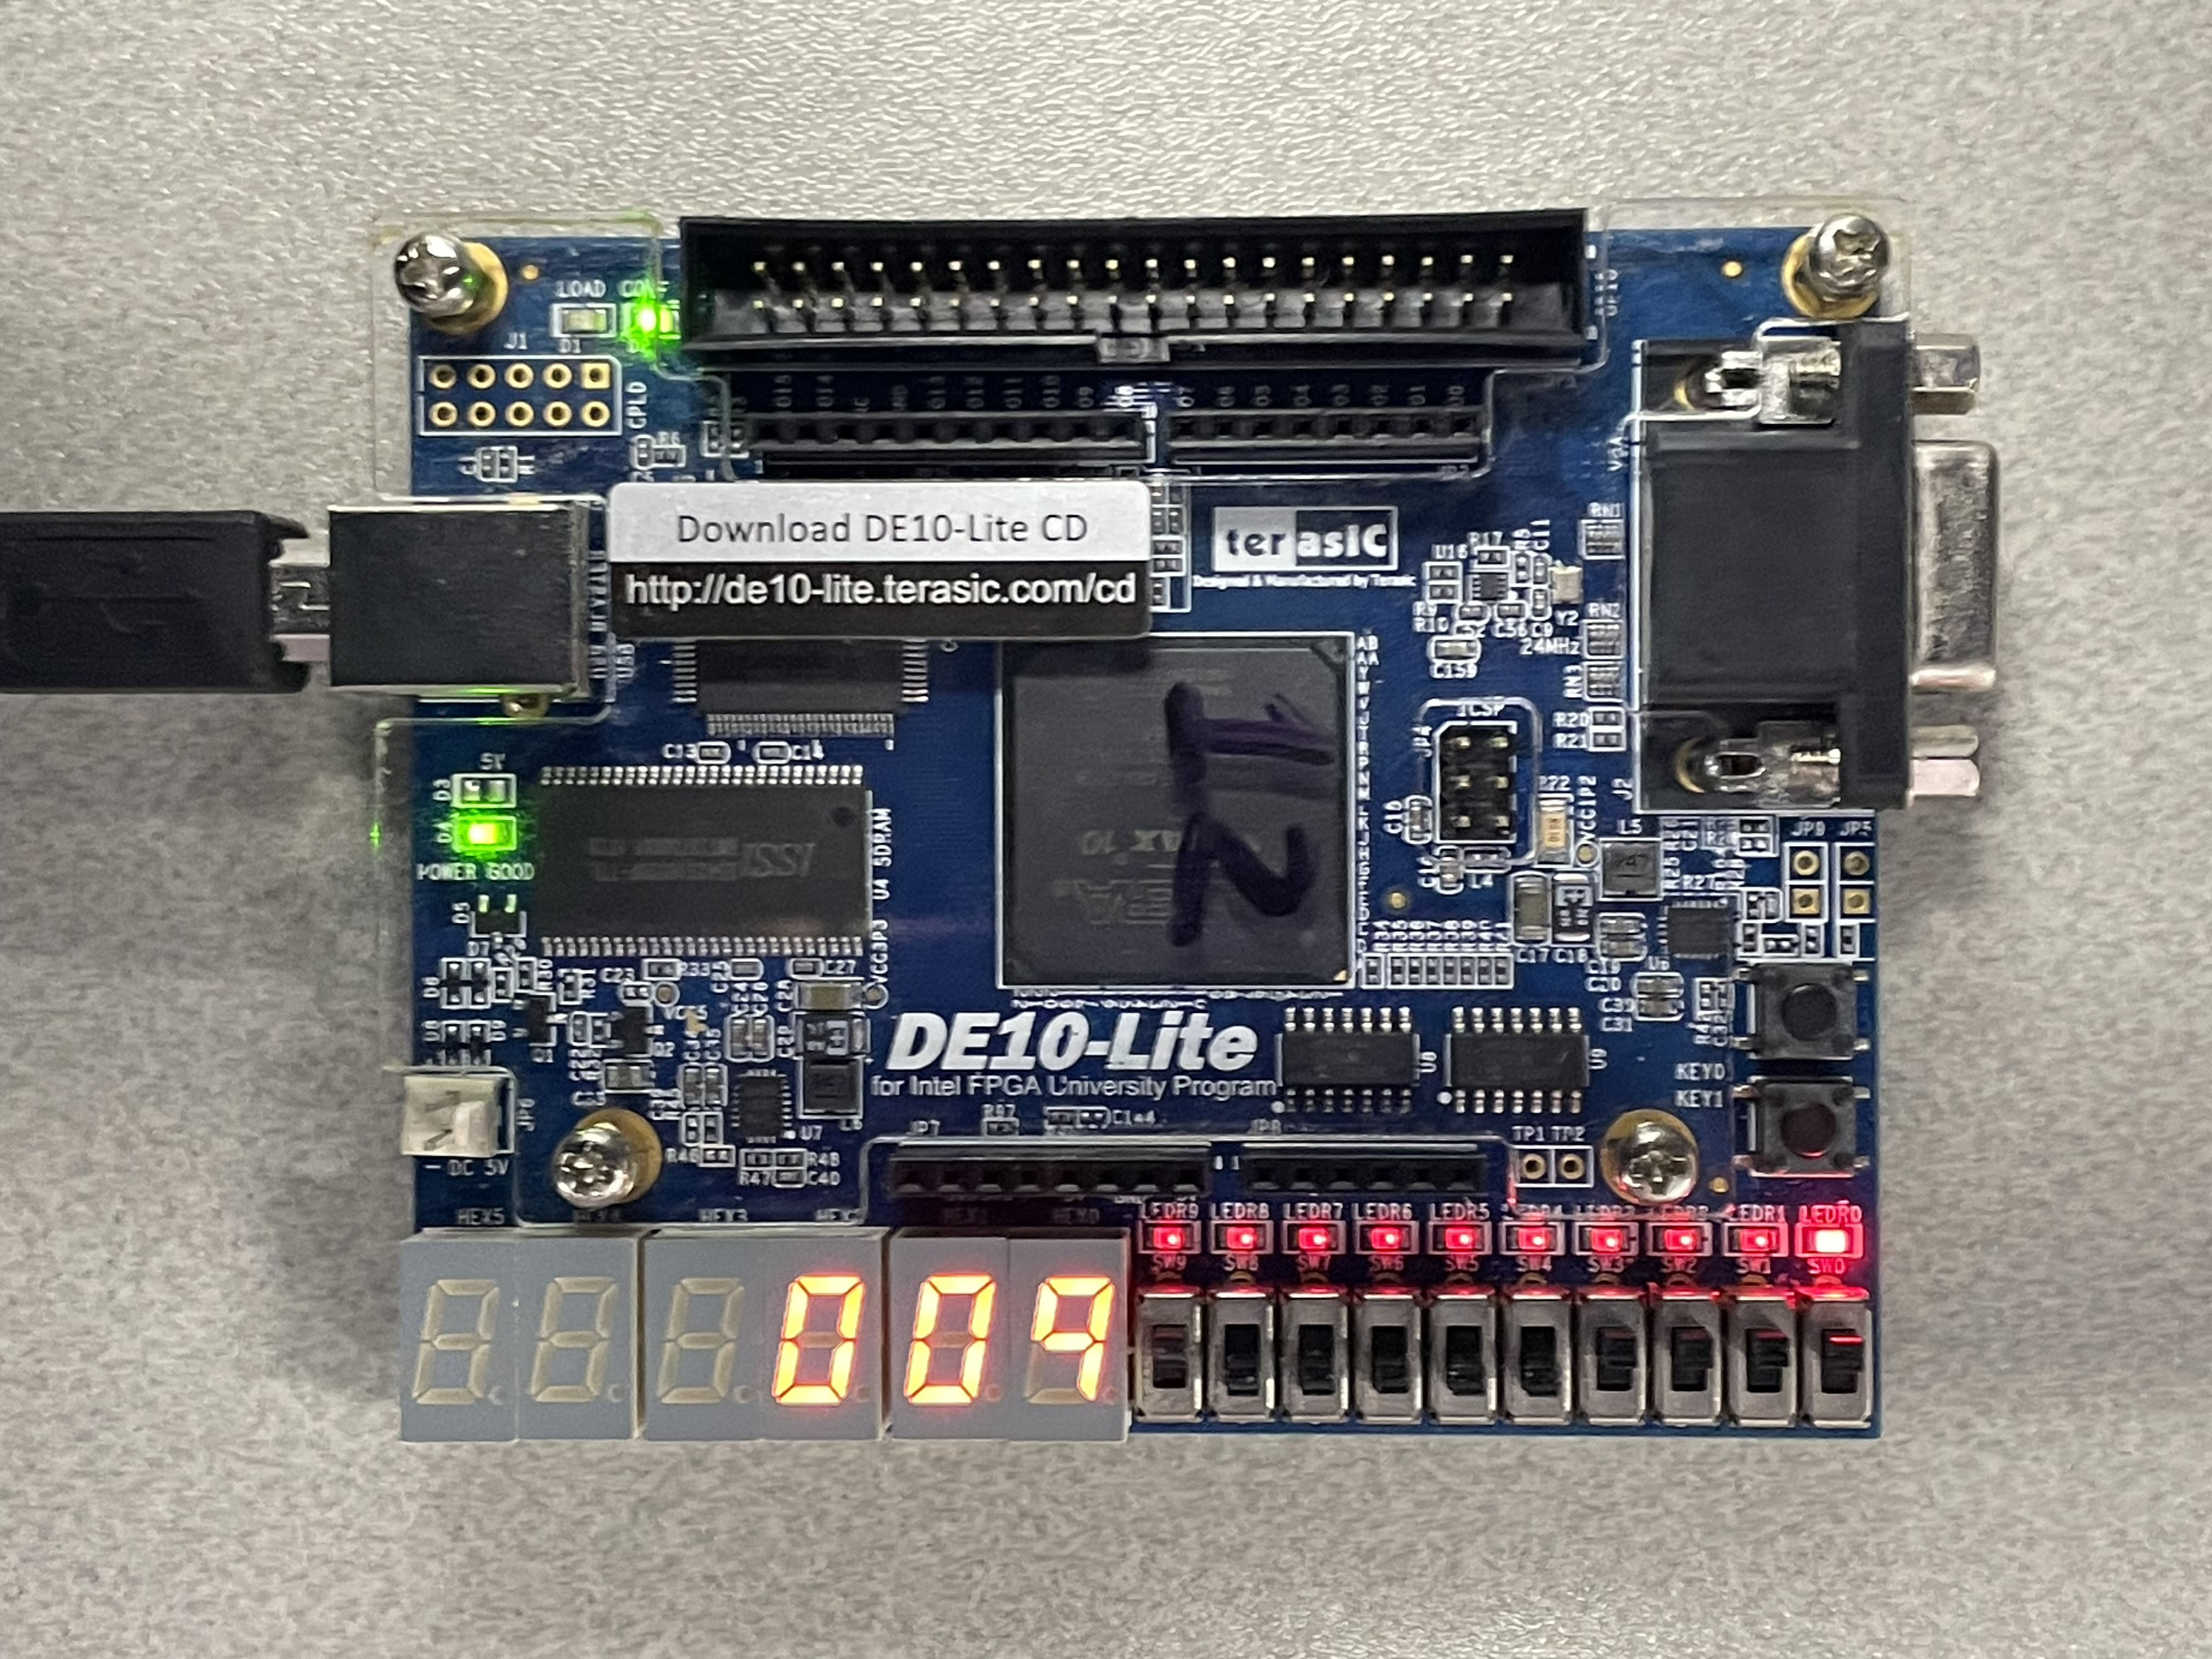
\includegraphics[width=.85\linewidth]{Montagem Laboratorial/images/IMG_2312.png}
        \caption{Teste na DE10-Lite (11)}\label{fig:DE11}
    \end{figure}
    \begin{figure}[H]
        \centering
        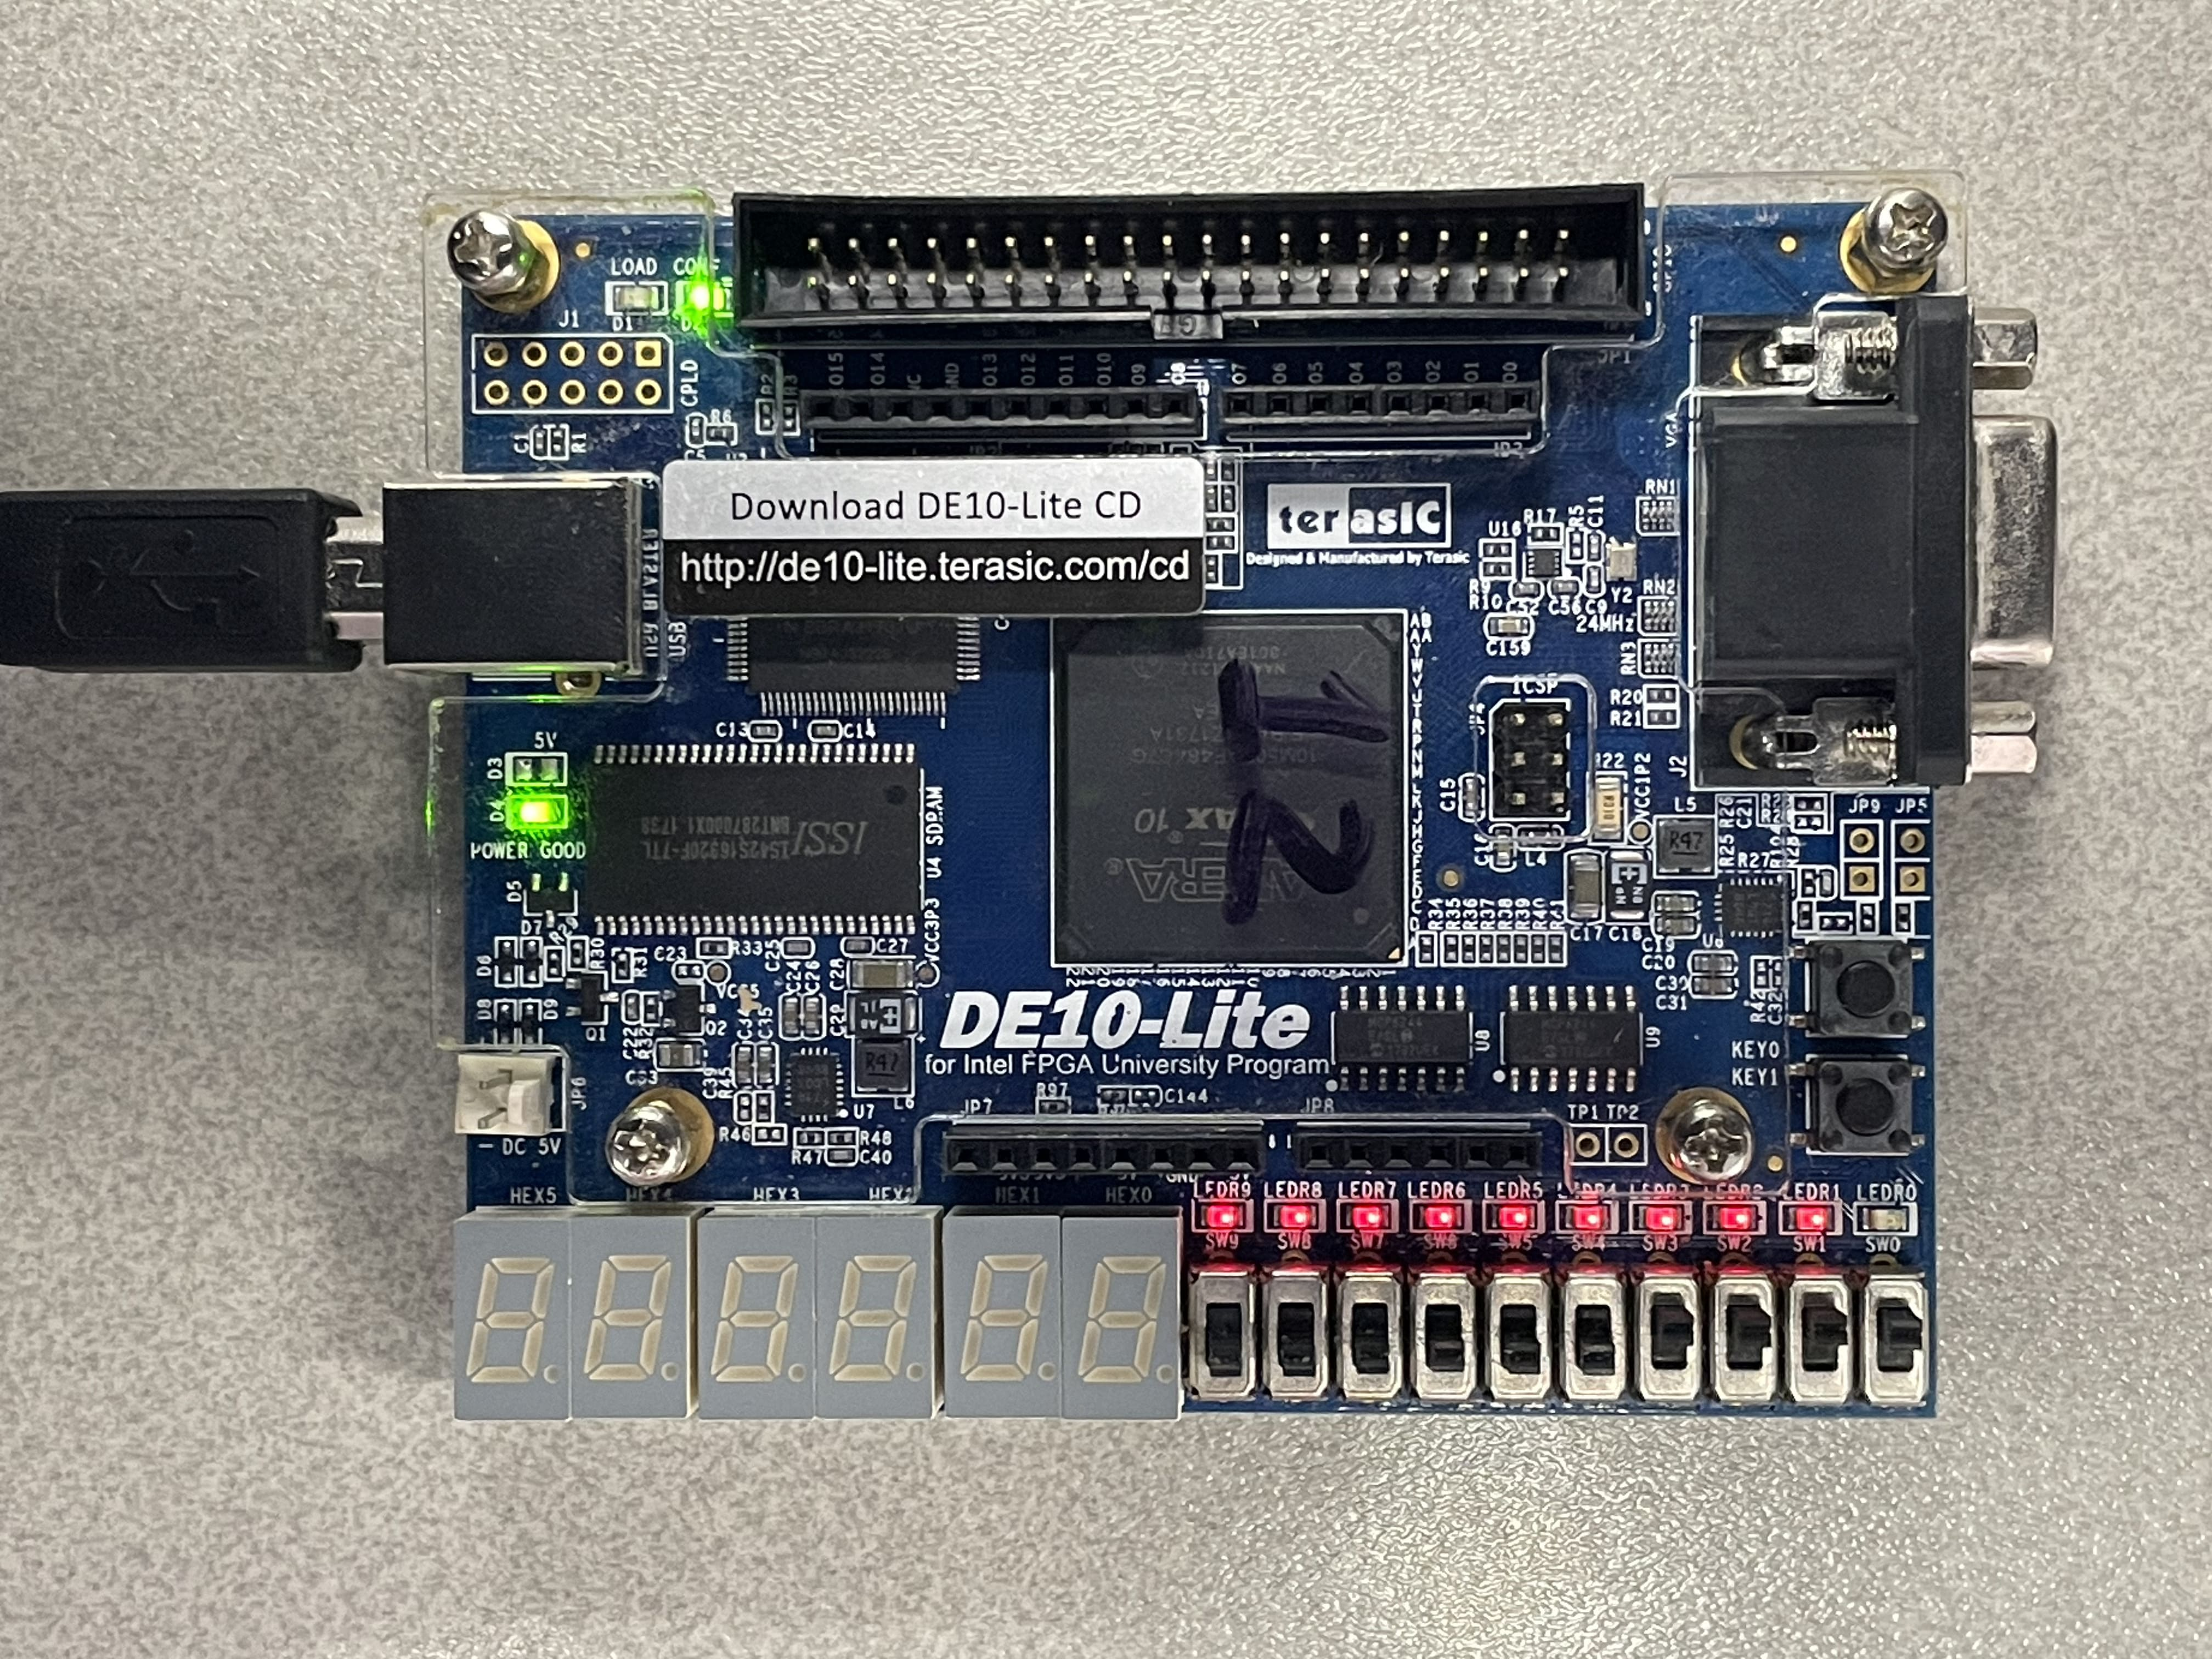
\includegraphics[width=.85\linewidth]{Montagem Laboratorial/images/IMG_2314.png}
        \caption{Teste na DE10-Lite (12)}\label{fig:DE12}
    \end{figure}
\end{multicols}

De seguida, na figura~\ref{fig:DE11}, desativamos o Step e obtemos o nosso valor acumulado. Neste momento o valor foi cortado na sua representação e, por isso, apenas mostra 9 $(265 - 256 \text{ (Inclui o Zero) }) = 9$. Temos agora um valor acumulado. Por último, na figura~\ref{fig:DE12}, o Start é desativado, retornando a placa ao seu estado inicial.

\vspace*{\fill}%